%=======================================================================
% abnTeX2: Modelo de Trabalho Acadêmico em conformidade com 
% ABNT NBR 14724:2011: Informação e documentação - Trabalhos acadêmicos
% Adaptado para o IFC
%=======================================================================

\PassOptionsToPackage{brazilian}{babel}
\documentclass[
    % -- opções da classe memoir --
    12pt,                 % tamanho da fonte    
    oneside,              % não imprimir em verso e anverso
    a4paper,              % tamanho do papel. 
    % -- opções da classe abntex2 --
    chapter=TITLE,        % títulos de capítulos em maiúsculas
    section=TITLE,        % títulos de seções em maiúsculas
    subsection=TITLE,     % títulos de subseções em maiúsculas
    % -- opções do pacote babel --
    english,              % idioma adicional para hifenização
    brazilian,            % idioma principal
    sumario=tradicional,
]{abntex2-IFC}

% Usa \input em vez de \include no preâmbulo para as configurações
% ---
% Pacotes fundamentais 
% ---
\usepackage[brazilian]{babel}    % Define o idioma do documento (resolve o erro do tracklang)
\usepackage{fontspec}            % Gerenciamento moderno de fontes
\setmainfont{Times New Roman}    % Fonte Times nativa para XeLaTeX/LuaLaTeX

\usepackage{lastpage}            % Usado pela Ficha catalográfica
\usepackage{indentfirst}         % Indenta o primeiro parágrafo de cada seção
\usepackage{color}               % Controle das cores
\usepackage{graphicx}            % Inclusão de gráficos
\usepackage{amsfonts}            % Símbolos

% ---- Ajuste no alinhamento das listas
\usepackage{enumitem}
\setitemize[0]{itemindent=0.4cm,itemsep=0pt}
\setenumerate[0]{itemindent=0.5cm,itemsep=0pt}

% Lista de Acrônimos (carregado DEPOIS do babel)
\usepackage[acronym, nomain, nonumberlist]{glossaries}
\makeglossaries

% ---
% Pacotes de citações e layout
% ---
\usepackage[brazilian,hyperpageref]{backref} % Páginas com as citações na bibl
\usepackage[a4paper]{geometry}

% Referência ABNT
\usepackage[alf,      
            abnt-emphasize=bf,
            abnt-url-package=none,
            abnt-repeated-title-omit=yes,
            abnt-full-initials=yes,
            abnt-etal-list=3
]{abntex2/abntex2cite}

\usepackage{lipsum}              % Para geração de dummy text
\usepackage{multirow}
\usepackage{float}
\usepackage{setspace}
\usepackage{tabularx}
\usepackage[table,xcdraw]{xcolor}

% Configurações de aparência do PDF final
\definecolor{blue}{RGB}{41,5,195}

% --- 
% Espaçamentos entre linhas e parágrafos 
% --- 
\setlength{\parindent}{2cm}
\linespread{1.5}

% Espaçamento depois dos títulos
\setlength{\afterchapskip}{\baselineskip}

% Controle do espaçamento entre um parágrafo e outro:
\setlength{\parskip}{0cm}

\hangcaption
\captionstyle[\raggedright]{}

% Desativa o texto de backref nas referências
\renewcommand{\backref}{}
\renewcommand*{\backrefalt}[4]{}

% Ajuste nas listas de tabela, ilustrações e quadros
\setlength\cftbeforechapterskip{0pt}

% ---
% Compila o índice
% ---
\makeindex

% Capa inserida antes do \begin{document}
% ---
% Informações de dados para CAPA e FOLHA DE ROSTO
% ---

\titulo{\uppercase{Desenvolvimento de ferramenta para cálculo e planejamento de redes ópticas de acesso}}
\autor{\uppercase{Everton José Serighelli}}
\local{Videira}
\data{2026}
\orientador[Orientador:]{Angelita Zanella}
\coorientador[Coorientador:]{Fabrício Bizotto}
\instituicao{ Ministério da Educação\\
        Secretaria de Educação Profissional e Tecnológica\\
        Instituto Federal Catarinense\\
        Câmpus Videira}
\tipotrabalho{Trabalho de Conclusão de Curso}
% O preambulo deve conter o tipo do trabalho, o objetivo, 
% o nome da instituição e a área de concentração
\preambulo{Trabalho de Conclusão de Curso apresentado ao
Curso de graduação em Ciência da Computação do
Instituto Federal Catarinense – Câmpus Videira para
obtenção do título de bacharel em Ciência da Computação.

Orientador: \imprimirorientador

Coorientador: \imprimircoorientador}
% ---



\begin{document}

% Retira espaço extra obsoleto entre as frases
\frenchspacing 

% ----------------------------------------------------------
% ELEMENTOS PRÉ-TEXTUAIS
% ----------------------------------------------------------

% CAPA
\imprimircapa

% FOLHA DE ROSTO
\imprimirfolhaderosto

% FOLHA DE APROVAÇÃO
\include{pretextuais/folhadeaprovacao}

% DEDICATÓRIA, AGRADECIMENTOS E EPÍGRAFE
\include{pretextuais/dedicatoria}
\include{pretextuais/agradecimentos}
% \include{pretextuais/epigrafe} % Reativar quando o arquivo for adicionado.

% RESUMO
\include{pretextuais/resumo}

% LISTA DE ILUSTRAÇÕES
\pdfbookmark[0]{\listfigurename}{lof}
\listoffigures*
\cleardoublepage

% LISTA DE QUADROS (Se necessário descomentar)
%\pdfbookmark[0]{\listofquadrosname}{loq}
%\listofquadros*
%\cleardoublepage

% LISTA DE TABELAS (Se necessário descomentar)
%\pdfbookmark[0]{\listtablename}{lot}
%\listoftables*
%\cleardoublepage

% ACRÔNIMOS E SIGLAS
\newacronym{ifc}{IFC}{Instituto Federal Catarinense}
\newacronym[longplural={sistemas de detecção de intrusão}, 
            firstplural={Sistemas de Detecção de Intrusão (IDS, do ingl\^es \emph{Intrusion Detection System})}, 
            first={Sistema de Detecção de Intrusão (IDS, do ingl\^es \emph{Intrusion Detection System})}
            ]{ids}{IDS}{sistema de detecção de intrusão}

\newacronym{pon}{PON}{\textit{Passive Optical Network}}
\newacronym{ftth}{FTTH}{\textit{Fiber To The Home}}
\newacronym{mvc}{MVC}{\textit{Model, View and Controller}}
\newacronym{olt}{OLT}{\textit{Optical Line Transmissor}}
\newacronym{cto}{CTO}{\textit{Customer Terminal Outlet}}
\newacronym[
    first={{{Caixas de Terminação Óptica (CTOs, do inglês (\textit{Customer Terminal Outlet}))}}},
    longplural={{{Caixas de Terminação Óptica}}}
]{cto2}{CTO}{{Caixa de Terminação Óptica}}


\newacronym{odn}{ODN}{\textit{Optical Distribution Network}}
\newacronym[longplural=ONUs]{onu}{ONU}{\textit{Optical Network Unit}}
\newacronym{ont}{ONT}{\textit{Optical Network Terminal}}
\newacronym{http}{HTTP}{\textit{Hypertext Transfer Protocol}}
\newacronym{api}{API}{\textit{Application Programming Interface}}
\newacronym{rest}{REST}{\textit{Representational State Transfer}}
\newacronym{json}{JSON}{\textit{JavaScript Object Notation}}
\newacronym{gis}{GIS}{\textit{Geographic Information System}}
\newacronym{sfp}{SFP}{\textit{Small Form-factor Pluggable}}
\newacronym{gbic}{GBIC}{\textit{Gigabit Interface Converter}}
\newacronym{uri}{URI}{\textit{Uniform Resource Identifier}}
\newacronym{epon}{EPON}{\textit{Ethernet Passive Optical Network}}
\newacronym{gpon}{GPON}{\textit{Gigabit Passive Optical Network}}
\newacronym{xgpon}{XG-PON}{10-\textit{Gigabit-capable Passive Optical Network}}
\newacronym{xgspon}{XGS-PON}{10-\textit{Gigabit Symmetric Passive Optical Network}}
\newacronym{html}{HTML}{\textit{HyperText Markup Language}}
\newacronym{svg}{SVG}{\textit{Scalable Vector Graphics}}
\newacronym{css}{CSS}{\textit{Cascading Style Sheets}}
\newacronym{ia}{IA}{Inteligência Artificial}
\newacronym{cnpq}{CNPq}{Conselho Nacional de Desenvolvimento Científico e Tecnológico}
\newacronym{mec}{MEC}{Ministério da Educação}
\newacronym{spa}{SPA}{Single Page Application}

\renewcommand*{\acronymname}{LISTA DE ABREVIATURAS E SIGLAS}
\newglossarystyle{mylong}{%
  \setglossarystyle{long}%
  \renewenvironment{theglossary}%
     {\begin{longtable}[l]{@{}p{\dimexpr 2cm-\tabcolsep}p{0.8\hsize}}}
     {\end{longtable}}%
}

% Corrigido: Vírgula adicionada entre Acronyms e type=acronym
\printglossary[toctitle=Acronyms, type=acronym, style=mylong, title=LISTA DE ABREVIATURAS E SIGLAS]
\newpage

% SUMÁRIO
\pdfbookmark[0]{\contentsname}{toc}
\tableofcontents*
\cleardoublepage

% ------------------------------------------------------
% ELEMENTOS TEXTUAIS
% ------------------------------------------------------
\textual

\chapter{Introdução} 
A crescente demanda por serviços de banda larga tem impulsionado o desenvolvimento e a consolidação de tecnologias de acesso mais eficientes, destacando-se as redes ópticas baseadas em arquitetura \gls{pon} como solução predominante para conexões \gls{ftth}. Em comparação aos meios metálicos tradicionais, a infraestrutura de fibra óptica viabiliza maior largura de banda, imunidade a interferências eletromagnéticas e baixa atenuação do sinal ao longo da propagação. Entretanto, o planejamento dessas redes envolve cálculos técnicos detalhados, especialmente relacionados ao orçamento óptico, o que pode tornar o processo complexo e suscetível a erros.

O dimensionamento de redes ópticas \gls{pon} exige a consideração de diversos elementos técnicos, como a potência transmitida pela \gls{olt}, as perdas introduzidas por fibras ópticas, conectores, fusões e \textit{splitters}, bem como a topologia adotada ao longo da rede. Conforme apresentado por \citeonline{keiser2011pon}, a correta análise do orçamento óptico é essencial para garantir que o sinal chegue ao usuário final dentro dos limites de potência recomendados. Quando esses cálculos são realizados manualmente, o processo tende a ser demorado e sujeito a falhas, sobretudo em projetos com múltiplos componentes distribuídos geograficamente. Dessa forma, a ausência de ferramentas automatizadas e visuais pode comprometer a eficiência e a confiabilidade do planejamento das redes \gls{ftth}.

Para mitigar tais limitações, propõe-se o desenvolvimento de uma aplicação web interativa voltada à modelagem e análise de redes ópticas \gls{pon}. A ferramenta permitirá ao usuário projetar a topologia da rede de forma visual, realizar cálculos de orçamento óptico e avaliar a viabilidade do projeto antes de sua implementação. Desse modo, busca-se auxiliar profissionais e empresas do setor de telecomunicações na tomada de decisão, reduzindo erros de dimensionamento, custos operacionais e tempo de planejamento.

\section{Problema}
O planejamento de redes ópticas baseadas na arquitetura \gls{pon} envolve a análise de múltiplos parâmetros técnicos, como topologia da rede, distribuição de componentes passivos e cálculo do orçamento óptico. Na prática, esses processos são frequentemente realizados de forma manual, por meio de planilhas e diagramas não integrados, o que torna o planejamento demorado, suscetível a erros e de difícil visualização. Embora existam ferramentas para esse fim, muitas delas são voltadas principalmente ao registro físico ou geográfico dos elementos da rede, ou se baseiam no uso de planilhas, apresentando limitações quanto à integração entre modelagem visual e análise de desempenho. Assim, a ausência de soluções que integrem, de maneira automatizada e visual, a modelagem da topologia e o cálculo do orçamento óptico dificulta a validação técnica dos projetos e compromete a eficiência do planejamento de redes \gls{ftth}.

\section{Objetivo Geral}
Desenvolver uma aplicação web interativa que integre a modelagem visual da topologia de redes ópticas \gls{pon} ao cálculo automático do orçamento óptico, fornecendo uma solução que auxilie o planejamento, a análise e a validação técnica de projetos de redes \gls{ftth}.

\section{Objetivos Específicos}
Para atingir o objetivo geral proposto, este trabalho foi dividido em um conjunto de objetivos específicos que orientam o desenvolvimento da aplicação web. Esses objetivos contemplam tanto os aspectos técnicos relacionados à modelagem e ao cálculo do orçamento óptico em redes \gls{pon} quanto as decisões arquiteturais e de usabilidade. São eles:

\begin{itemize}
  \item Projetar uma interface para a modelagem visual da topologia de redes ópticas \gls{pon}, possibilitando a inserção de elementos como \gls{olt}, caixas de emenda, \textit{splitters} e terminais de forma interativa.
  \item Implementar o cálculo automático do orçamento óptico, considerando perdas associadas à fibra óptica, conectores, fusões e divisores ópticos, conforme parâmetros técnicos definidos.
  \item Desenvolver uma interface dinâmica e interativa, utilizando a biblioteca D3.js para a visualização gráfica da topologia da rede e atualização em tempo real dos resultados.
  \item Estruturar o \textit{backend} da aplicação seguindo a arquitetura \gls{mvc}, disponibilizando os dados e resultados por meio de uma \gls{api} \textit{RESTful} e garantindo a separação entre lógica de negócio, dados e interface.
  \item Armazenar as informações da rede planejada em formato \gls{json}, permitindo o armazenamento, a recuperação e a reutilização dos projetos desenvolvidos na aplicação.
\end{itemize}

\section{Justificativa}

A expansão das redes ópticas de acesso, especialmente aquelas baseadas na arquitetura \gls{pon}, tem intensificado a necessidade de processos de planejamento mais precisos e eficientes. Nesse cenário, destacam-se os desafios relacionados ao cálculo do orçamento óptico, à definição adequada da topologia da rede e à validação técnica dos projetos desenvolvidos. Além disso, a complexidade crescente dessas redes exige ferramentas que auxiliem não apenas nos cálculos, mas também na compreensão estrutural do projeto. Assim, justifica-se a proposta de desenvolvimento de uma aplicação web que integre modelagem visual e cálculo automatizado no planejamento de redes \gls{ftth} \cite{keiser2011pon,oliviero2014fiber}.

Embora existam ferramentas voltadas ao planejamento de redes ópticas, muitas delas apresentam limitações quanto à integração entre cálculo técnico e representação da topologia da rede. Em geral, essas soluções não oferecem uma exibição clara e intuitiva que permita o rápido entendimento do projeto por parte do projetista e do técnico responsável pela implementação em campo. A ausência de representação adequada dificulta a compreensão de sistemas complexos e compromete a análise e a tomada de decisão \cite{munzner2014visualization}. Além disso, a falta de recursos interativos integrados aos dados técnicos dificulta a identificação de inconsistências no projeto e a comunicação entre as etapas de planejamento e execução, especialmente em redes mais complexas \cite{keiser2011pon,bostock2011d3}.

Nesse contexto, o desenvolvimento de uma aplicação \textit{web} que una visualização interativa e cálculos automáticos de orçamento óptico apresenta-se como uma solução adequada às demandas atuais. A automatização dos cálculos contribui para a redução de erros e para o aumento da confiabilidade do projeto, enquanto a representação gráfica da topologia permite uma compreensão mais rápida e precisa da rede planejada. A adoção de uma arquitetura baseada em \gls{api} \gls{rest}, conforme o estilo arquitetural proposto por \citeonline{fielding2000rest}, favorece a separação entre \textit{frontend} e \textit{backend} e contribui para a organização e escalabilidade do sistema. O armazenamento das informações em formato \gls{json}, definido como um padrão leve e amplamente utilizado para intercâmbio de dados estruturados, aliado à arquitetura \gls{mvc} e à utilização da biblioteca D3.js para visualização dinâmica, possibilita a construção de uma ferramenta flexível, organizada e alinhada às boas práticas de desenvolvimento de software \cite{bray2017json, bostock2011d3}.

\section{Estrutura do texto}

O presente trabalho está organizado de forma a apresentar, de maneira lógica e progressiva, os conceitos, a fundamentação teórica, o desenvolvimento da solução proposta e a análise dos resultados obtidos, com foco no planejamento de redes ópticas baseadas na arquitetura \gls{pon}. 

O Capítulo 2 contempla a fundamentação teórica, reunindo os principais conceitos relacionados às redes de acesso ópticas, arquitetura \gls{pon}, topologias de rede, cálculo do orçamento óptico e ferramentas de planejamento. Também são abordados conceitos de visualização de dados e arquiteturas de aplicações web, que fundamentam as escolhas tecnológicas adotadas na solução proposta. 

No Capítulo 3 é descrita a metodologia adotada no trabalho, incluindo a caracterização da pesquisa, a arquitetura da solução baseada em modelo cliente-servidor, as tecnologias empregadas e o processo de desenvolvimento da aplicação. Além disso, são apresentados os procedimentos definidos para a validação do sistema e análise dos resultados. 

O Capítulo 4 apresenta os trabalhos correlatos, discutindo soluções acadêmicas e ferramentas de mercado voltadas ao planejamento e gestão de redes \gls{ftth}. A análise comparativa permite identificar limitações existentes, especialmente quanto à integração entre visualização da topologia e cálculo do orçamento óptico, justificando a proposta desenvolvida neste estudo. 

Os capítulos subsequentes contemplam a apresentação dos resultados esperados, as discussões e as considerações finais do trabalho, nas quais são sintetizadas as contribuições da aplicação desenvolvida, suas limitações e sugestões para trabalhos futuros, reforçando sua relevância no contexto do planejamento de redes ópticas. 

A estrutura adotada busca garantir organização, clareza e coerência na apresentação do conteúdo, permitindo ao leitor compreender, de maneira progressiva, os aspectos teóricos, técnicos e práticos envolvidos no desenvolvimento da solução proposta.

\chapter{Fundamentação Teórica}

Para fundamentar a proposta apresentada, será apresentada a base teórica necessária para a compreensão dos conceitos técnicos e tecnológicos abordados neste trabalho. Inicialmente, serão discutidos os princípios das redes ópticas de acesso e da arquitetura \gls{pon}, bem como os elementos relacionados ao orçamento óptico e ao planejamento dessas redes. Também serão abordados aspectos relacionados às ferramentas e métodos atualmente utilizados, destacando suas limitações. Por fim, serão vistos conceitos de visualização de dados e arquiteturas de aplicações web que fundamentam as escolhas tecnológicas adotadas no desenvolvimento da solução proposta. 

\section{Redes de Acesso}

As redes de acesso constituem o segmento da infraestrutura de telecomunicações responsável por conectar a rede do provedor aos usuários finais, sejam eles residenciais ou corporativos. Diferentemente do núcleo de rede (\textit{core} ou \textit{backbone}), que realiza a interconexão entre centrais do provedor e a troca de tráfego com outros provedores, a rede de acesso tem como principal característica a capilaridade, uma vez que precisa alcançar um grande número de pontos finais distribuídos geograficamente. Ao longo do tempo, diversas tecnologias foram empregadas nesse segmento, evoluindo conforme as demandas por largura de banda, confiabilidade e qualidade de serviço \cite{tanenbaum2011networks}.

A separação funcional entre a rede \textit{core} e a rede de acesso pode ser observada de forma esquemática na Figura~\ref{fig:core_acesso}. Enquanto a rede \textit{backbone} concentra a responsabilidade pelo transporte de grandes volumes de dados em longas distâncias, promovendo a interligação entre \textit{datacenters}, centrais de comutação e pontos estratégicos da infraestrutura do provedor por meio de enlaces de alta capacidade. A rede de acesso representa o segmento mais capilar da rede de telecomunicações, sendo responsável por estabelecer a conexão direta entre os assinantes finais e os serviços oferecidos. Em razão dessa característica, a rede de acesso assume papel crítico no desempenho global da transmissão, concentrando os principais desafios técnicos associados à última milha\footnote{Trecho de fibra óptica entre o provedor e o assinante}, tais como limitações físicas do meio, elevada dispersão geográfica dos usuários e a necessidade de soluções que conciliem eficiência técnica, escalabilidade e viabilidade econômica. Por atender diretamente o assinante, esse segmento é particularmente sensível às limitações tecnológicas, sendo frequentemente o principal gargalo em termos de desempenho e capacidade quando tecnologias inadequadas são empregadas \cite{tanenbaum2011networks}.

\begin{figure}[htb]
	\caption{Diferença entre a rede \textit{core}/\textit{backbone} e a rede de acesso}
    \centering
    \parbox{16cm}{
        \centering
        \label{fig:core_acesso}
		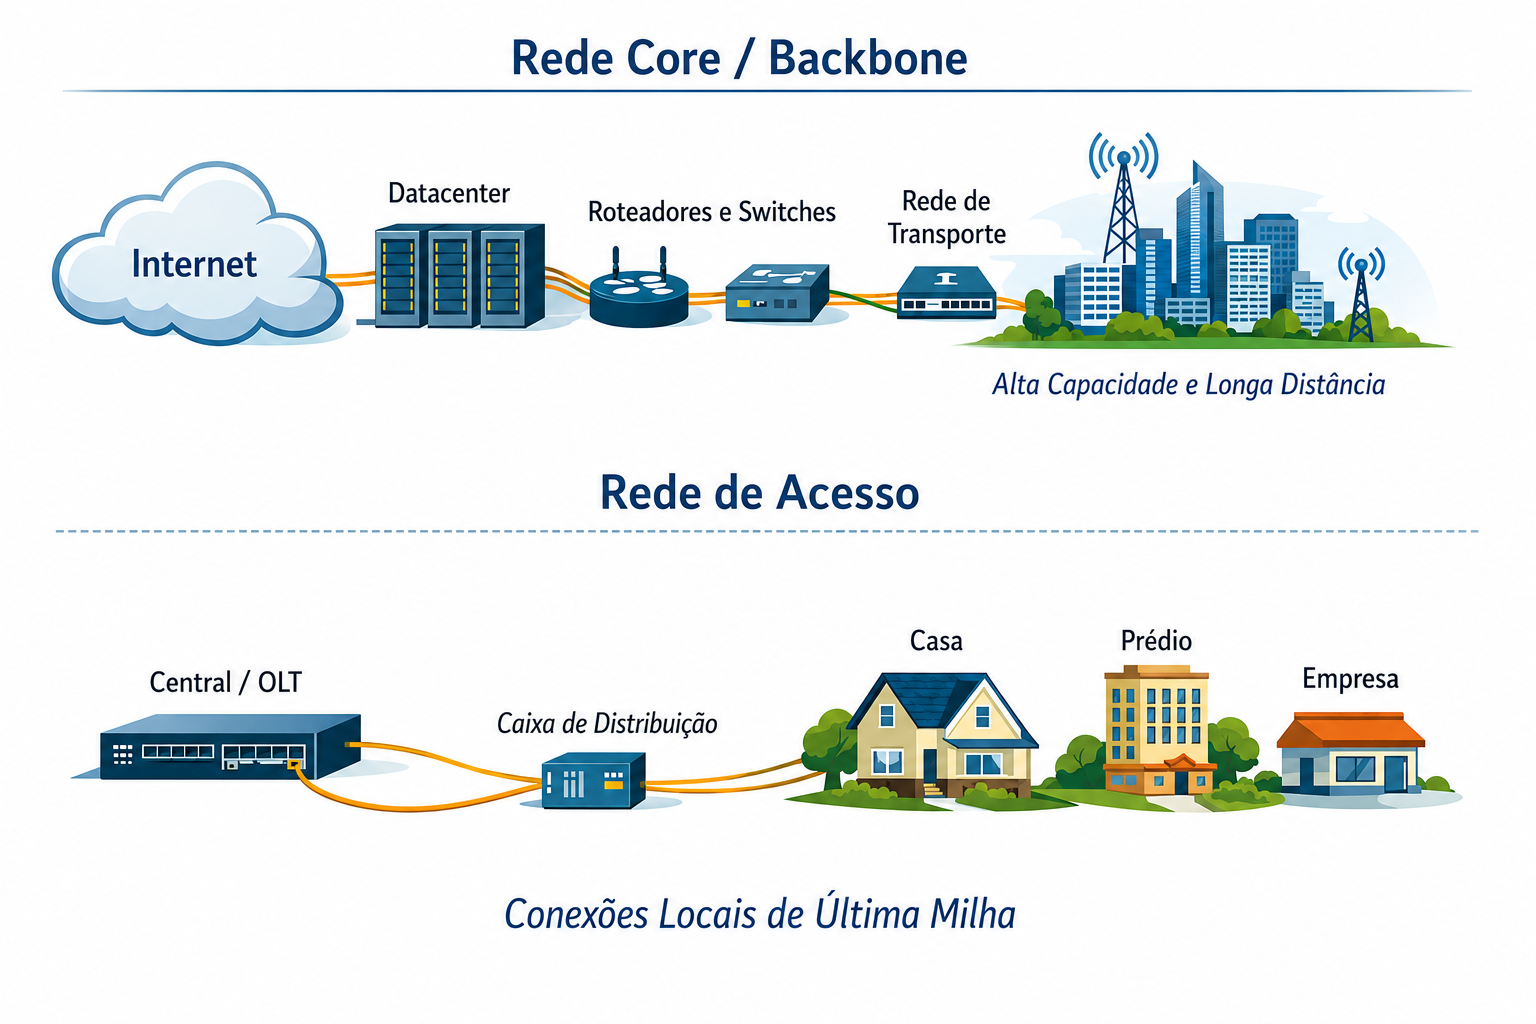
\includegraphics[width=\textwidth]{images/core_acesso.png}
	    \par\footnotesize Fonte: Elaboração própria com auxílio de \gls{ia}.
    }
\end{figure}

Historicamente, as primeiras soluções de acesso à rede de dados foram baseadas em tecnologias discadas sobre a infraestrutura telefônica existente, caracterizadas por baixas taxas de transmissão e forte dependência da qualidade das linhas metálicas. Com o aumento da demanda por serviços de dados, surgiram tecnologias baseadas em par metálico, como as variantes da família xDSL, que permitiram ampliar a capacidade de transmissão utilizando a mesma infraestrutura de cobre da telefonia. Apesar de representarem um avanço significativo em relação ao acesso discado, essas tecnologias apresentaram limitações inerentes ao meio físico, como maior atenuação, suscetibilidade a interferências e forte dependência da distância entre o usuário e a central \cite{tanenbaum2011networks}.

Paralelamente às soluções cabeadas, tecnologias de acesso sem fio também foram amplamente utilizadas. Especialmente em cenários nos quais a implantação de infraestrutura física apresentava restrições econômicas ou geográficas. Sistemas baseados em rádio, redes Wi-Fi de longo alcance e tecnologias celulares possibilitaram ampliar o acesso à conectividade, mostrando-se úteis para expandir a cobertura de serviços em áreas remotas de baixa densidade populacional ou com infraestrutura limitada. Contudo, em muitos casos, essas soluções apresentam limitações relacionadas à capacidade compartilhada, interferências e variabilidade do desempenho. Embora permaneçam relevantes em determinados contextos, o crescimento contínuo do consumo de dados evidenciou a necessidade de meios de acesso com maior capacidade e estabilidade \cite{tanenbaum2011networks}.

Nesse cenário, a fibra óptica passou a ser amplamente reconhecida como a solução mais adequada para redes de acesso de alta capacidade \cite{oliviero2014fiber,keiser2011pon}. Esse meio físico utiliza pulsos de luz para transportar informações ao longo de um filamento de vidro ou plástico de alta pureza, oferecendo vantagens expressivas em relação aos meios metálicos, como elevada largura de banda, menor atenuação do sinal e imunidade a interferências eletromagnéticas \cite{keiser2011pon}. Essas características tornam essa tecnologia especialmente apropriada para atender às exigências atuais e futuras de tráfego, tanto em ambientes residenciais quanto corporativos.

A adoção da fibra óptica no segmento de acesso, possibilitou o surgimento de diferentes modelos de implantação, entre os quais se destaca o \gls{ftth}. O termo \gls{ftth}, refere-se à estratégia de levar a fibra óptica até as dependências do usuário final, seja em residências ou empresas, caracterizando uma rede de acesso totalmente óptica no último trecho da infraestrutura. Essa abordagem elimina as limitações associadas a soluções híbridas ou baseadas em cobre, proporcionando maior desempenho, confiabilidade e escalabilidade para o atendimento às crescentes demandas por serviços de banda larga \cite{oliviero2014fiber}.

Para viabilizar tecnicamente as implantações \gls{ftth} em larga escala, são adotadas arquiteturas de rede específicas, entre as quais se destaca a \gls{pon}. Diferentemente do \gls{ftth}, que define o alcance físico da fibra até o usuário final, a arquitetura \gls{pon} consiste em um padrão arquitetural de rede óptica de acesso baseado na distribuição do sinal em topologia ponto–multiponto por meio de componentes passivos\footnote{Dispositivos que não precisam de energia elétrica}, como fibras e \textit{splitters}, entre a central do provedor e os terminais dos usuários. A ausência de elementos ativos\footnote{Dispositivos que precisam de energia elétrica} no trecho de distribuição contribui para a redução de custos operacionais, aumento da confiabilidade e simplificação da manutenção, tornando a arquitetura \gls{pon} amplamente empregada em redes \gls{ftth} modernas~\cite{keiser2011pon}.

\section{Arquitetura \gls{pon}}

A arquitetura \gls{pon} organiza a rede de acesso a partir de uma topologia ponto-multiponto, na qual um único enlace proveniente da central do provedor é compartilhado entre múltiplos usuários finais. Essa arquitetura fundamenta-se na separação funcional entre elementos ativos e passivos ao longo da infraestrutura, definindo a forma como o sinal óptico é gerado, distribuído e entregue aos assinantes. Em virtude dessa organização, a \gls{pon} se tornou a principal arquitetura empregada na implementação de redes \gls{ftth} em larga escala \cite{itutg9841,keiser2011pon}.

A organização dos elementos que compõem a arquitetura \gls{pon} pode ser visualizada na Figura~\ref{fig:arquitetura_pon}. Observa-se que os componentes ativos concentram-se nas extremidades da rede, com a \gls{olt} localizada na central do provedor e as unidades \gls{onu}/\gls{ont} junto aos usuários finais, enquanto a \gls{odn} é formada exclusivamente por elementos passivos, como fibras ópticas, caixas de emenda e \textit{splitters}. Essa característica de distribuição passiva dispensa alimentação elétrica intermediária ao longo do trecho de atendimento, simplificando a infraestrutura de campo e reduzindo significativamente os pontos potenciais de falha física \cite{keiser2011pon}.

\begin{figure}[htb]
	\caption{Arquitetura de uma rede \gls{pon} baseada em topologia ponto--multiponto}
    \centering
    \parbox{16cm}{
        \centering
        \label{fig:arquitetura_pon}
		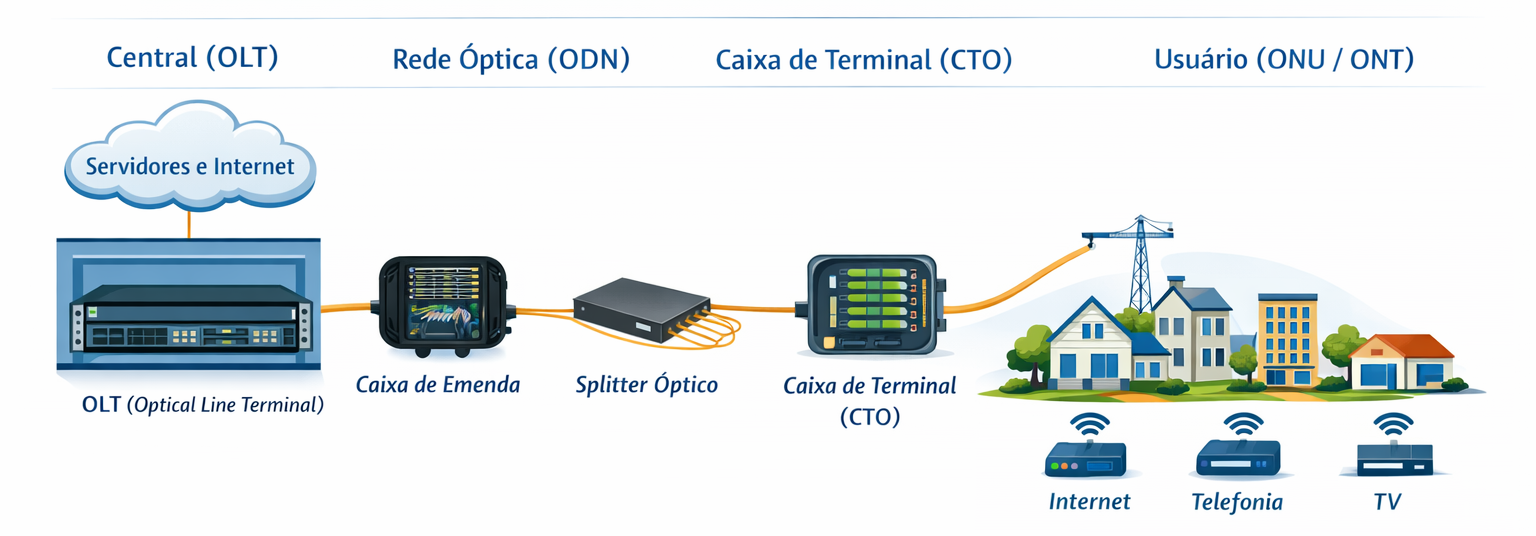
\includegraphics[width=\textwidth]{images/arquitetura_pon.png}
	    \par\footnotesize Fonte: Elaboração própria com auxílio de \gls{ia}.
    }
\end{figure}

A geração inicial do sinal óptico na arquitetura \gls{pon} é realizada por meio de transceptores instalados na \gls{olt}. Esses transceptores, normalmente implementados em módulos do tipo \gls{sfp} ou equivalentes, realizam a conversão do sinal elétrico em óptico e definem parâmetros essenciais da transmissão, como potência de saída, comprimento de onda e sensibilidade de recepção. A partir desses módulos, o sinal gerado é lançado na rede e passa a ser compartilhado entre múltiplos usuários por meio dos componentes passivos da rede de distribuição \cite{keiser2011pon,itutg9842}.

Entre a \gls{olt} (provedor) e as \gls{onu} (clientes) encontra-se a Rede de Distribuição Óptica (\gls{odn}), composta exclusivamente por elementos passivos, como fibras ópticas, \textit{splitters}, caixas de emenda e caixas de terminação. Esses componentes não realizam processamento do sinal nem conversão eletro-óptica, limitando-se à condução e à divisão do sinal luminoso ao longo da topologia da rede. Por ser uma estrutura inteiramente passiva, o desempenho desse trecho da infraestrutura está condicionado estritamente às características físicas de propagação e atenuação dos materiais instalados, o que torna o planejamento e a modelagem matemática dessa seção fatores críticos para a viabilidade técnica \cite{itutg9841,keiser2011pon}. 

As caixas de emenda desempenham papel fundamental na \gls{odn}, sendo utilizadas para a proteção e organização das fusões ópticas entre cabos ao longo do trajeto de distribuição. Essas caixas não realizam atendimento direto aos usuários finais, mas garantem a continuidade do enlace óptico e facilitam a manutenção e possíveis reconfigurações da rede, salvaguardando a integridade das conexões físicas \cite{foa_splice_closure}. Por sua vez, o atendimento aos assinantes ocorre por meio das \gls{cto2},  posicionadas estrategicamente próximas aos usuários e destinadas à conexão dos cabos de derivação (\textit{drop cables}) às unidades finais, organizando o último trecho da rede \gls{ftth} \cite{cto_ftth_distribution,cto_fibracem}.

Embora apresente diversas vantagens, a arquitetura \gls{pon} exige um planejamento criterioso da topologia, da posição dos \textit{splitters} e da distribuição das caixas de emenda e de \gls{cto} ao longo da rede. A divisão excessiva do sinal óptico ou o posicionamento inadequado desses elementos pode comprometer os níveis de potência recebidos pelos usuários finais \cite{keiser2011pon}. Por isso, a análise do orçamento óptico torna-se essencial para garantir o desempenho e a confiabilidade de toda a estrutura. Além dos aspectos relacionados à transmissão de luz, o desempenho e a eficiência geral da rede também estão diretamente associados à forma como sua topologia de distribuição é organizada ao longo da \gls{odn}, influenciando decisões de projeto e o uso da infraestrutura física disponível \cite{keiser2011pon,oliviero2014fiber}.

\section{Topologias Balanceadas e Desbalanceadas em Redes \gls{pon}}

No contexto da arquitetura \gls{pon}, a organização da topologia de distribuição do sinal óptico pode ser classificada, de forma geral, como balanceada ou desbalanceada. Essa classificação está relacionada à forma como o sinal é dividido ao longo da rede e influencia tanto o planejamento lógico quanto a utilização da infraestrutura física disponível \cite{keiser2011pon,itutg9841}.

Em topologias balanceadas, a divisão do sinal ocorre de maneira uniforme entre as diferentes ramificações, resultando em caminhos ópticos com características semelhantes de atenuação e comprimento. Essa abordagem simplifica o planejamento inicial da rede e a validação do orçamento óptico, uma vez que os enlaces tendem a apresentar condições similares de potência recebida. No entanto, esse modelo de distribuição frequentemente demanda um maior número de fibras ópticas ativas ao longo dos cabos de distribuição, pois múltiplas ramificações precisam ser atendidas de forma equivalente desde os níveis iniciais da \gls{odn} \cite{keiser2011pon,oliviero2014fiber}.

Por outro lado, em topologias desbalanceadas, a divisão do sinal é realizada de forma assimétrica, permitindo que determinadas ramificações da rede recebam maior potência óptica ou sejam priorizadas em função da distribuição geográfica dos usuários e da expansão progressiva do atendimento. Em implantações \gls{ftth} reais, essa abordagem é amplamente adotada, pois possibilita maior flexibilidade de projeto e tende a utilizar um número menor de fibras ópticas nos cabos de distribuição, uma vez que nem todos os pontos de atendimento exigem a mesma capacidade ou extensão desde os níveis iniciais da rede \cite{keiser2011pon}.

\begin{figure}[htb]
	\caption{Comparação entre topologias balanceada e desbalanceadas em redes \gls{pon}}
	\label{fig:topologias_pon}
    \centering
    \parbox{16cm}{
		\centering
		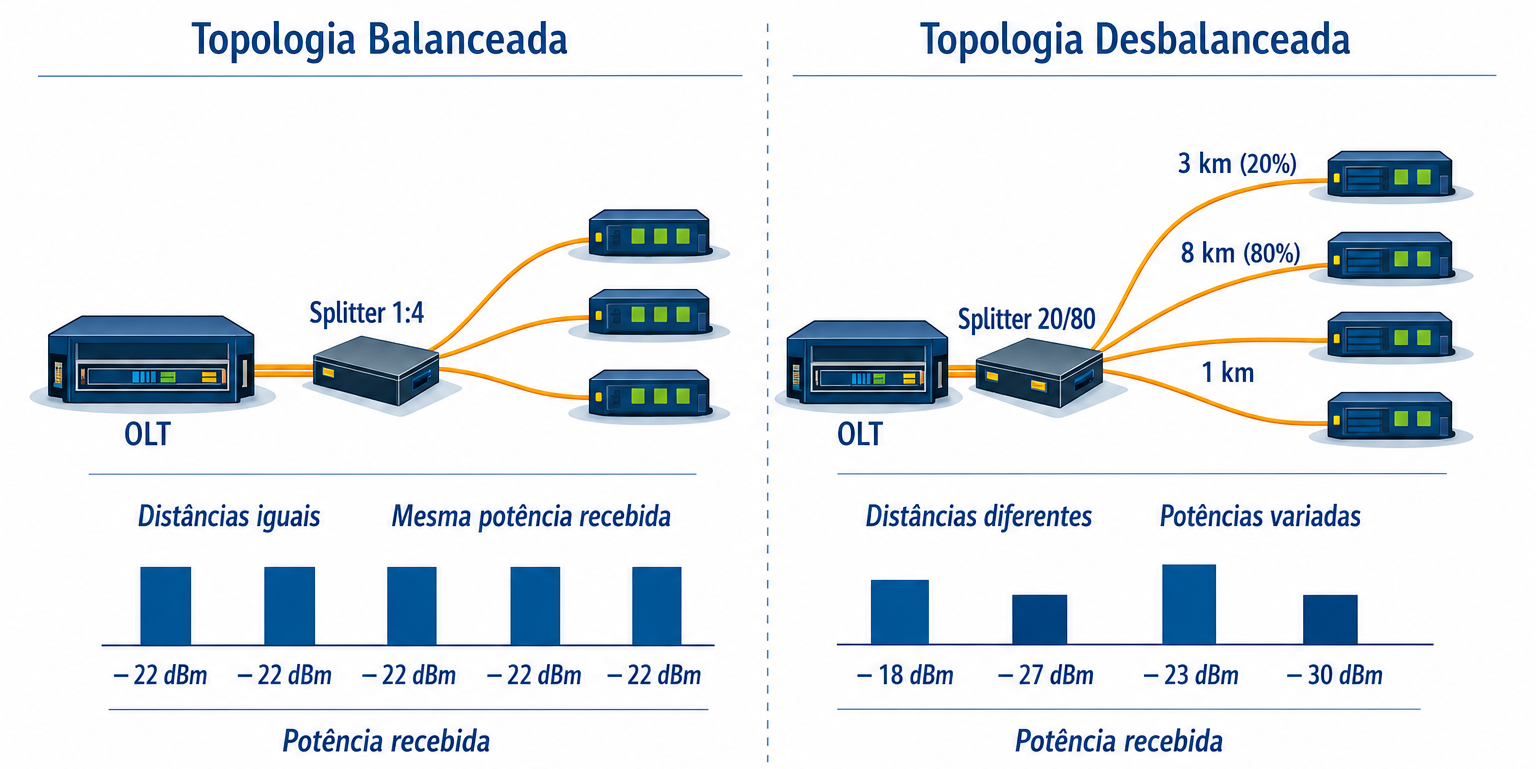
\includegraphics[width=\textwidth]{images/topologias_pon.png}
		\par\footnotesize Fonte: Elaboração própria com auxílio de \gls{ia}.
    }
\end{figure}

A distinção entre as abordagens balanceada e desbalanceadasa em redes \gls{pon} pode ser observada na Figura~\ref{fig:topologias_pon}. No modelo balanceado, as ramificações apresentam extensões semelhantes, resultando em níveis de potência recebida praticamente equivalentes nos terminais finais, o que simplifica o planejamento e a validação do orçamento óptico. Em contrapartida, na distribuição desbalanceada, os enlaces possuem comprimentos distintos, ocasionando diferentes níveis de atenuação e, consequentemente, potências recebidas variáveis, o que permite maior flexibilidade no projeto da rede, porém exige uma análise individualizada do orçamento óptico para cada ramificação \cite{keiser2011pon}.

Dessa forma, a escolha entre topologias balanceadas e desbalanceadas envolve um compromisso entre simplicidade de planejamento, balanceamento de potência e eficiência no uso da infraestrutura física. Independentemente da topologia adotada, torna-se essencial avaliar o orçamento óptico de forma adequada para cada ramificação final, garantindo que todos os enlaces atendam aos limites operacionais estabelecidos pelos equipamentos ativos utilizados \cite{apnic_gpon_budget}. Além da organização topológica da rede, a arquitetura \gls{pon} também é definida pelos padrões tecnológicos adotados, os quais estabelecem limites de capacidade e de divisão do sinal, influenciando diretamente o dimensionamento da rede de acesso \cite{itutg9841,itu_optical_access_tutorial}.

\section{Padrões \gls{pon} e Capacidade de Divisão}

Diversos padrões de redes ópticas passivas são utilizados em implantações \gls{ftth}, entre os quais se destacam \gls{epon}, \gls{gpon}, \gls{xgpon} e \gls{xgspon}. Eles se diferem principalmente em aspectos como taxas de transmissão, comprimentos de onda utilizados e capacidade de atendimento. Entretanto, independentemente do padrão adotado, o princípio fundamental da arquitetura \gls{pon} permanece o mesmo.\cite{keiser2011pon,itutg9841}.

Do ponto de vista do planejamento do orçamento, é importante destacar que a metodologia de cálculo é conceitualmente idêntica para todos os padrões \gls{pon}. Em todos os casos, a margem é determinada pela diferença entre a potência de transmissão do equipamento de origem e a sensibilidade mínima de recepção do terminal, considerando-se as perdas acumuladas ao longo do caminho. Assim, a tecnologia \gls{pon} adotada não altera a lógica matemática da rede, mas define os limites e parâmetros operacionais dentro dos quais esse cálculo deve ser realizado \cite{keiser2011pon,holight_optical_budget}.

As principais diferenças entre os padrões \gls{pon} refletem-se nos limites normativos associados à capacidade do sistema, especialmente na taxa máxima de divisão do sinal suportada pela arquitetura. Esse parâmetro influencia diretamente o número máximo de ramificações que podem ser atendidas por uma única porta da \gls{olt}, impactando decisões de projeto relacionadas à topologia física, à distribuição dos \textit{splitters} e à densidade de atendimento \cite{itutg9841,itu_optical_access_tutorial}.

A Tabela~\ref{tab:padroes_pon_divisao} apresenta uma relação entre alguns dos principais padrões \gls{pon} e as taxas máximas típicas de divisão adotadas em projetos de redes \gls{ftth}, conforme práticas amplamente referenciadas na literatura técnica e em recomendações normativas \cite{itutg9841,keiser2011pon,itu_optical_access_tutorial}.

\begin{table}[htb]
\centering
\caption{Padrões \gls{pon} e taxas máximas típicas de divisão}
\label{tab:padroes_pon_divisao}
\begin{tabular}{c c}
\hline
\textbf{Padrão \gls{pon}} & \textbf{Taxa máxima típica de divisão} \\
\hline
Epon      & até 1$\times$64 \\
Gpon      & até 1$\times$128 \\
XG-pon    & até 1$\times$128 \\
XGS-pon   & até 1$\times$128 \\
\hline
\end{tabular}
\par\footnotesize Fonte: Adaptado de \cite{itutg9841} e \cite{keiser2011pon}.
\end{table}

A capacidade de divisão do sinal óptico varia de acordo com a tecnologia \gls{pon} adotada, conforme ilustrado na Figura~\ref{fig:epon_gpon_divisao}. No padrão \gls{epon}, uma única fibra pode ser compartilhada entre até 64 usuários finais, enquanto na arquitetura \gls{gpon} essa capacidade é ampliada, possibilitando a divisão do sinal para até 128 clientes. Essa diferença de escala determina a concentração de assinantes por porta física na central, definindo o nível de compartilhamento do meio físico e orientando a distribuição geográfica dos elementos passivos de derivação \cite{itutg9841,itu_optical_access_tutorial}.

\begin{figure}[htb]
	\caption{Comparação entre os padrões \gls{epon} e \gls{gpon} quanto à capacidade de divisão}
    \centering
    \parbox{16cm}{
		\centering
        \label{fig:epon_gpon_divisao}
		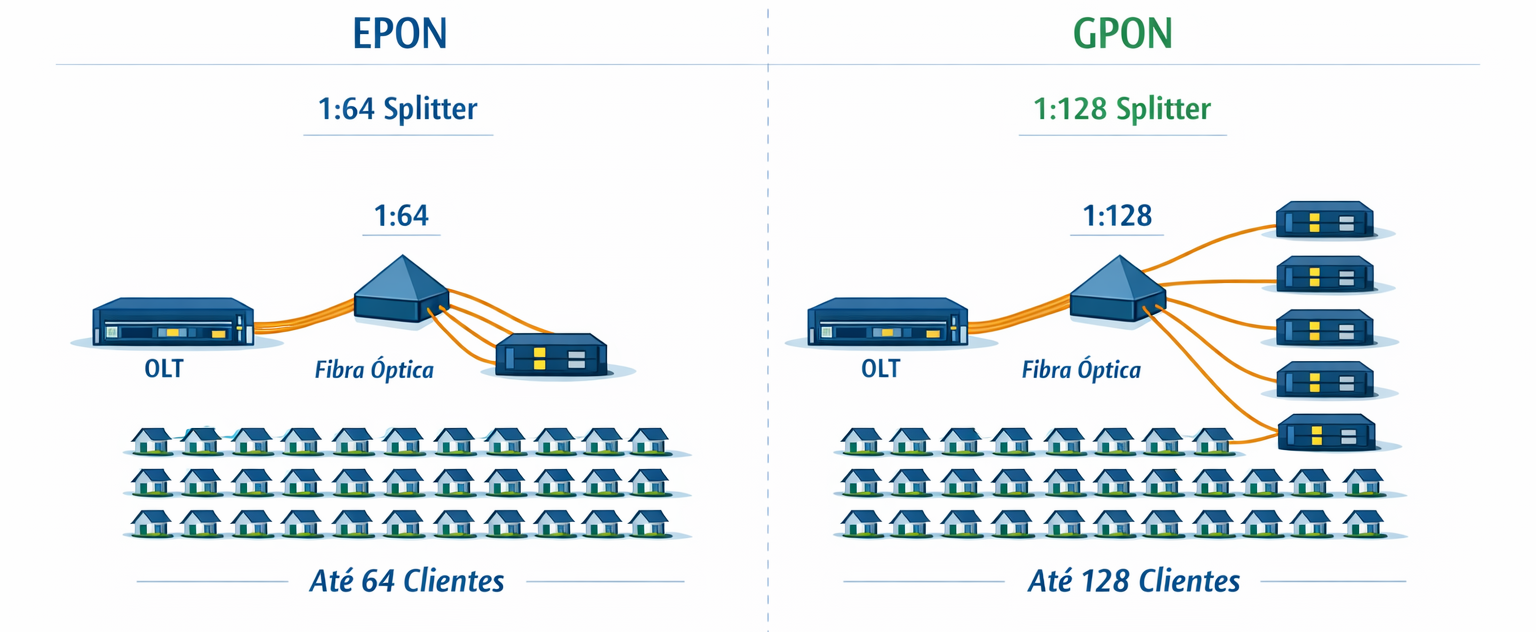
\includegraphics[width=\textwidth]{images/epon_gpon_divisao.png}
		\par\footnotesize Fonte: Elaboração própria com auxílio de \gls{ia}.
    }
\end{figure}

Dessa forma, a escolha da tecnologia \gls{pon} está associada principalmente à capacidade de atendimento e aos limites arquiteturais da infraestrutura, enquanto o cálculo do orçamento óptico permanece baseado nos mesmos fundamentos físicos. Essa característica reforça a importância de abordagens de planejamento que permitam a parametrização do padrão tecnológico adotado, possibilitando avaliar diferentes cenários de divisão e expansão do atendimento sem alterar a lógica fundamental do cálculo do orçamento \cite{keiser2011pon,holight_optical_budget}.

\section{Orçamento Óptico em Redes \gls{pon}}

O orçamento constitui um dos aspectos centrais no planejamento de redes baseadas na arquitetura \gls{pon}, pois está diretamente relacionado à garantia de que o sinal chegue ao usuário final dentro dos níveis adequados de potência. Em infraestruturas \gls{ftth}, nas quais o sinal é compartilhado entre múltiplos assinantes por meio de componentes passivos, a correta avaliação das perdas ao longo do enlace torna-se essencial para assegurar o desempenho e a confiabilidade do sistema \cite{keiser2011pon}. Nesse contexto, a análise do orçamento envolve a consideração de fatores como os limites de potência definidos pelos transceptores, a atenuação da fibra óptica, as perdas introduzidas por dispositivos passivos e conexões, bem como critérios normativos associados à transmissão.

Do ponto de vista físico, essa análise pode ser estruturada seguindo o percurso do sinal desde sua geração nos transceptores da \gls{olt} até a recepção nas unidades terminais, considerando-se, ao longo do trajeto, as perdas acumuladas pelos diferentes elementos da infraestrutura \cite{keiser2011pon,apnic_gpon_budget}.

\begin{figure}[htb]
	\caption{Consolidação das perdas no enlace óptico em redes \gls{pon}}
	\label{fig:perdas_consolidadas_enlace}
    \centering
    \parbox{16cm}{
		\centering
		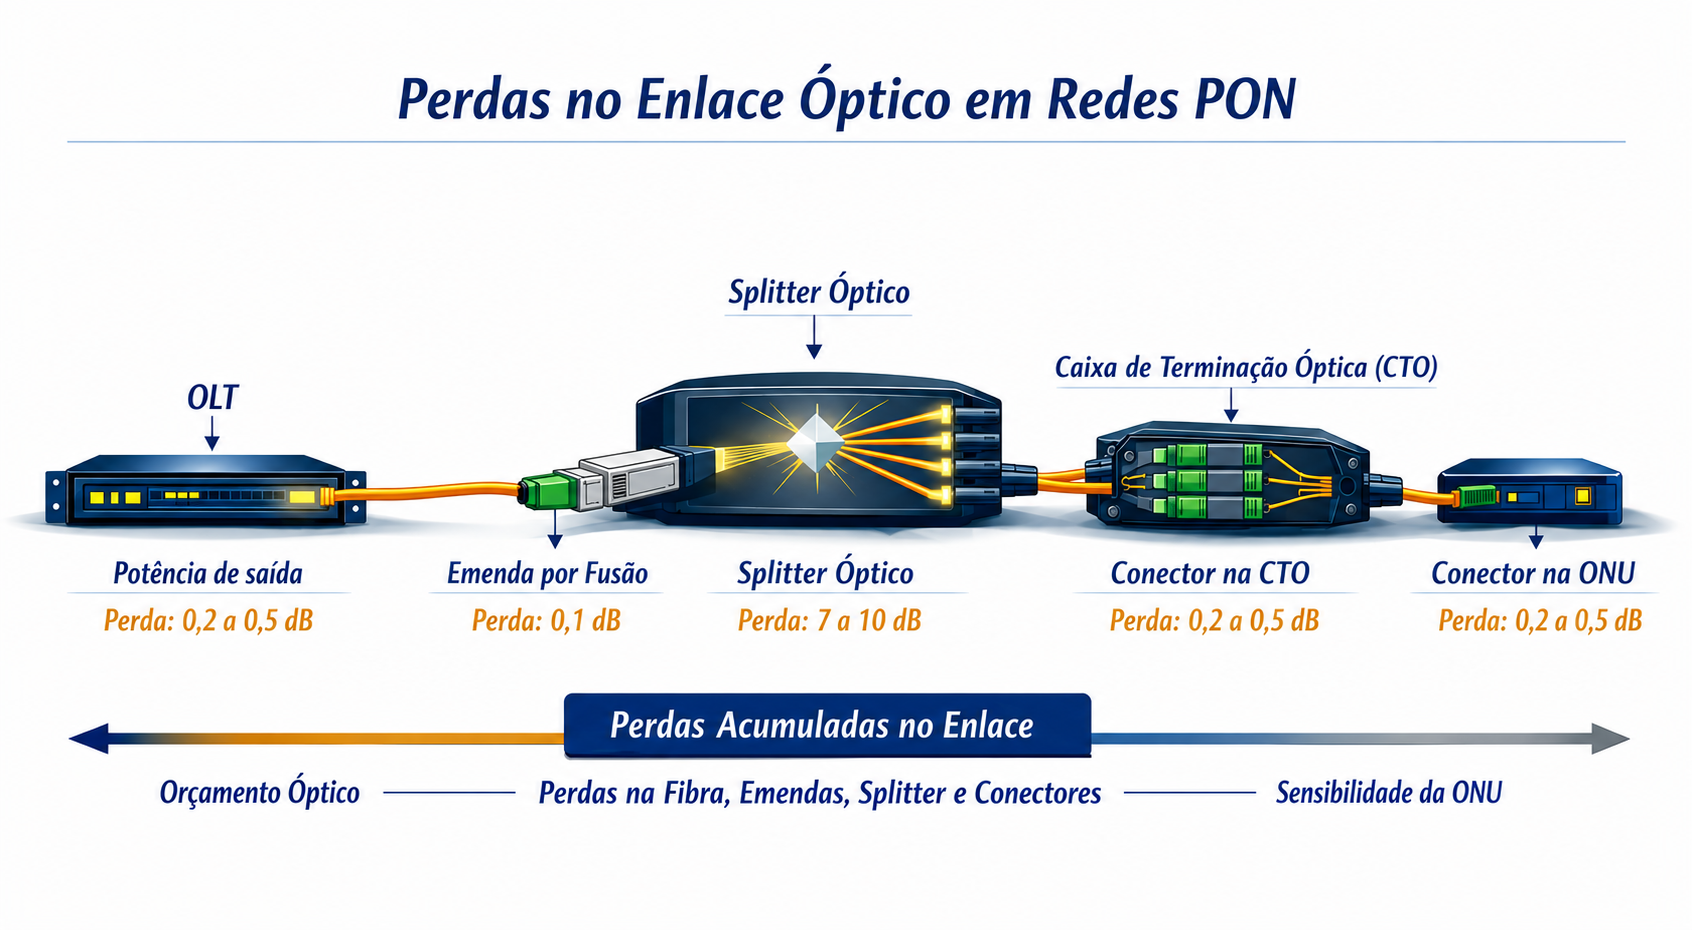
\includegraphics[width=\textwidth]{images/perdas_consolidadas_enlace.png}
		\par\footnotesize Fonte: Elaboração própria com auxílio de \gls{ia}.
    }
\end{figure}

A Figura~\ref{fig:perdas_consolidadas_enlace} apresenta uma visão global das atenuações incidentes ao longo de um enlace típico em redes \gls{pon}. Observa-se que a atenuação total resulta da soma de perdas distribuídas na fibra óptica e das perdas concentradas introduzidas por emendas, \textit{splitters} e conectores presentes na \gls{olt}, nas caixas de terminação e nas unidades \gls{onu}. A consolidação desses fatores é fundamental para a verificação do orçamento, uma vez que o enlace somente será considerado viável se a potência recebida no terminal final permanecer acima de sua sensibilidade mínima especificada \cite{keiser2011pon,holight_optical_budget}.

De forma conceitual, o orçamento pode ser entendido como a diferença entre a potência de transmissão (\textit{Tx}) e a sensibilidade mínima do receptor (\textit{Rx}), representando a perda máxima admissível para que o enlace permaneça ativo \cite{holight_optical_budget}. Em termos práticos, a validação do enlace é realizada comparando a capacidade de tolerar perdas com a perda total do caminho, que resulta da soma das atenuações introduzidas por componente ao longo do trajeto \cite{apnic_gpon_budget}. Quando a perda total excede a margem disponível, a potência recebida tende a ficar abaixo do limiar necessário e o enlace pode apresentar degradação de desempenho ou falhas de conexão \cite{holight_optical_budget}.

\subsection{Classes Ópticas e Transceptores \gls{pon}}

Os sistemas \gls{pon} utilizam transceptores instalados na \gls{olt} e nas unidades terminais (\gls{onu}/\gls{ont}) para realizar a transmissão e a recepção dos sinais. Esses componentes são normalmente implementados em módulos do tipo \gls{sfp} ou \gls{gbic}, que integram os elementos responsáveis pela emissão do feixe luminoso e pela detecção do sinal recebido. As características desses módulos, em especial a potência de transmissão (\textit{Tx}) e a sensibilidade de recepção (\textit{Rx}), exercem influência direta sobre a margem de atenuação disponível no enlace \cite{keiser2011pon,itutg9842}.

Nas redes \gls{gpon}, os transceptores são classificados em diferentes categorias de desempenho, como B+, C+ e C++, conforme definidas pelas recomendações da ITU-T \cite{itutg9842}. Cada classe estabelece limites mínimos de potência de transmissão e máximos de sensibilidade de recepção, determinando, assim, a perda total máxima admissível entre a \gls{olt} e as \gls{onu}. Dessa forma, a especificação adotada impõe restrições diretas à extensão máxima da rede, à taxa de divisão do sinal e à complexidade da topologia que pode ser suportada \cite{itutg9841,itutg9842}.

A Tabela~\ref{tab:classes_opticas_gpon} apresenta valores típicos de potência de transmissão, sensibilidade de recepção e margem de atenuação associados às principais classes de tranceptores utilizadas em sistemas \gls{gpon}, amplamente adotados como referência no planejamento de redes \gls{ftth} \cite{apnic_gpon_budget}.

\begin{table}[htb]
\centering
\caption{Classes ópticas \gls{gpon} e parâmetros típicos}
\label{tab:classes_opticas_gpon}
\begin{tabular}{c c c c}
\hline
\textbf{Classe óptica} & \textbf{Tx mín. (dBm)} & \textbf{Rx mín. (dBm)} & \textbf{Orçamento típico (dB)} \\
\hline
B+  & +1,5  & -28  & 29,5 \\
C+  & +3,0  & -32  & 35 \\
C++ & +5,0  & -35  & 40 \\
\hline
\end{tabular}
\par\footnotesize Fonte: Elaborado pelo autor com base em \cite{apnic_gpon_budget} e \cite{holight_optical_budget}.
\end{table}

Conforme apresentado na Tabela~\ref{tab:classes_opticas_gpon}, classes mais elevadas disponibilizam maior orçamento óptico, suportando enlaces mais longos, maiores taxas de divisão e topologias mais complexas, incluindo configurações com múltiplos estágios de \textit{splitters} ou topologias desbalanceadas. Por outro lado, os transceptores dessas classes apresentam maior custo, tornando a escolha uma decisão de projeto que envolve o equilíbrio entre desempenho técnico e viabilidade econômica \cite{keiser2011pon}.

\begin{figure}[htb]
	\caption{Conexão do transceptor óptico à porta \gls{sfp} da \gls{olt}}
	\label{fig:transceiver_sfp_olt}
    \centering
    \parbox{16cm}{
		\centering
		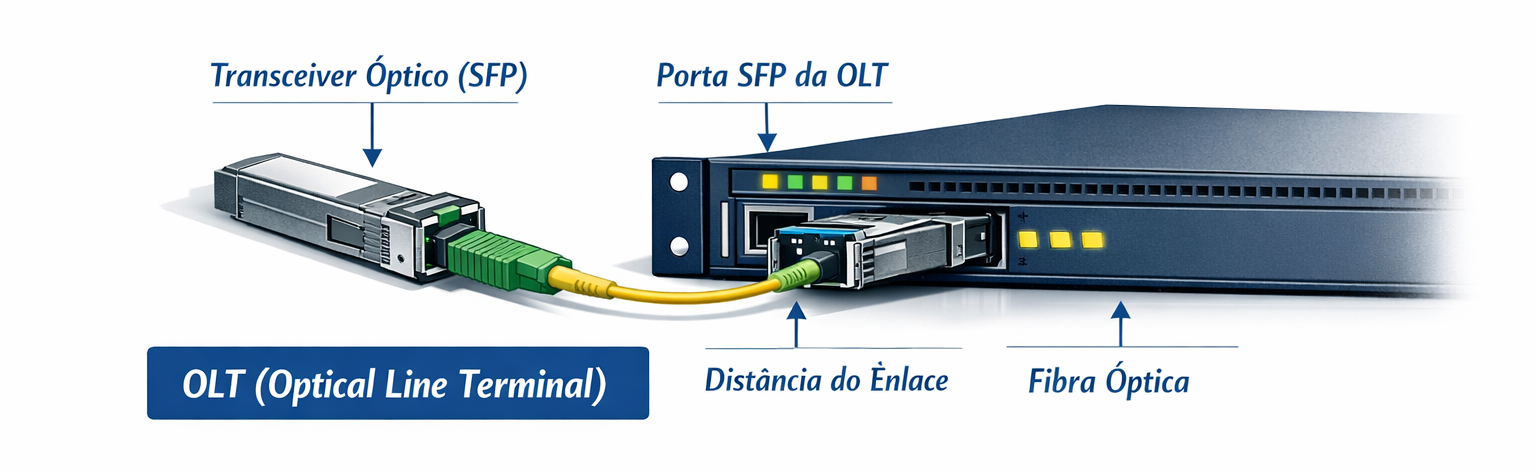
\includegraphics[width=\textwidth]{images/transceiver_sfp_olt.png}
		\par\footnotesize Fonte: Elaboração própria com auxílio de \gls{ia}.
    }
\end{figure}

A geração do sinal luminoso em redes \gls{pon} ocorre na \gls{olt} por meio de transceptores conectados às suas portas do tipo \gls{sfp}, conforme ilustrado na Figura~\ref{fig:transceiver_sfp_olt}. Esses módulos são responsáveis pela conversão do sinal elétrico em óptico, além de definirem parâmetros essenciais da transmissão, como potência de saída, comprimento de onda e alcance máximo do enlace. A partir do transceptor, o sinal é acoplado à fibra e lançado na \acrlong{odn}, dando início ao processo de atendimento aos usuários finais.

No contexto do planejamento de redes \gls{ftth}, a correta consideração da classe do transceptor é fundamental para garantir que o orçamento calculado seja compatível com os limites operacionais dos equipamentos utilizados. Assim, a definição adequada da classe selecionada, em conjunto com a modelagem das perdas ao longo da rede, constitui um elemento central para a validação técnica e a confiabilidade do projeto da rede \gls{pon}. Neste trabalho, esses valores são apresentados como referência teórica; o protótipo permite informar diretamente a potência de transmissão e a sensibilidade de recepção de cada equipamento, sem selecionar automaticamente uma classe normativa.

\subsection{Perdas Distribuídas: Atenuação da Fibra Óptica}

A atenuação total em um enlace \gls{pon} pode ser organizada em perdas distribuídas e concentradas. As primeiras estão associadas principalmente à atenuação natural do sinal na fibra óptica e variam conforme o comprimento de onda e as características do cabo, conforme descrito em recomendações técnicas \cite{itutg652_2024}. 

No caso da atenuação da fibra, especificações técnicas associadas indicam limites típicos de atenuação, como valores em torno de 0{,}30~dB/km  \cite{prysmian_g652d_datasheet}. Assim, o comprimento do enlace e a faixa de operação impactam diretamente o orçamento, tornando necessário planejar trajetos coerentes com a infraestrutura instalada e com as metas de divisão do sinal \cite{itutg652_2024}.

\begin{figure}[htb]
	\caption{Atenuação do sinal ao longo da fibra óptica em função da distância}
	\label{fig:atenuacao_fibra}
    \centering
    \parbox{16cm}{
		\centering
		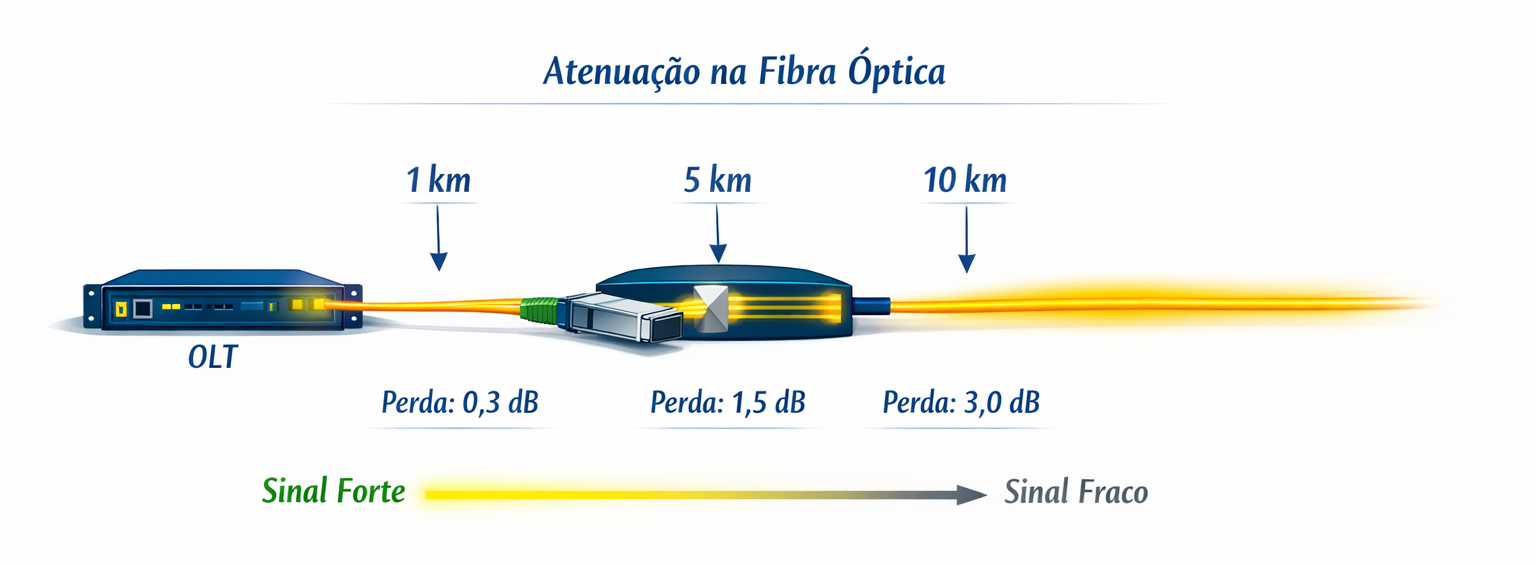
\includegraphics[width=\textwidth]{images/atenuacao_fibra.png}
		\par\footnotesize Fonte: Elaboração própria com auxílio de \gls{ia}.
    }
\end{figure}

A atenuação constitui uma perda distribuída ao longo do enlace, crescendo proporcionalmente ao comprimento do cabo empregado. Essa relação pode ser observada na Figura~\ref{fig:atenuacao_fibra}, na qual se evidencia que, à medida que a distância aumenta, ocorre a redução progressiva da potência do sinal. Em projetos de redes \gls{pon}, essa atenuação natural representa um dos fatores fundamentais no cálculo do orçamento óptico, devendo ser considerada conjuntamente com as perdas introduzidas por conectores, emendas e \textit{splitters}.

\subsection{Perdas Concentradas: \textit{Splitters}}

A divisão do sinal na arquitetura \gls{pon} é realizada por meio de \textit{splitters}, inseridos ao longo da \acrlong{odn}, conforme ilustrado na Figura~\ref{fig:splitter_optico }. Esses dispositivos recebem a portadora proveniente da \gls{olt} por uma única fibra de entrada e realizam a divisão da potência em múltiplas saídas, distribuindo o sinal para diferentes ramificações. Por se tratarem de elementos totalmente passivos, os \textit{splitters} não requerem alimentação elétrica e contribuem para a redução de custos operacionais e o aumento da confiabilidade dos sistemas de acesso \gls{pon}.

\begin{figure}[htb!]
	\caption{Funcionamento do \textit{splitter} e divisão do sinal em redes \gls{pon}}
	\label{fig:splitter_optico }
    \centering
    \parbox{16cm}{
		\centering
		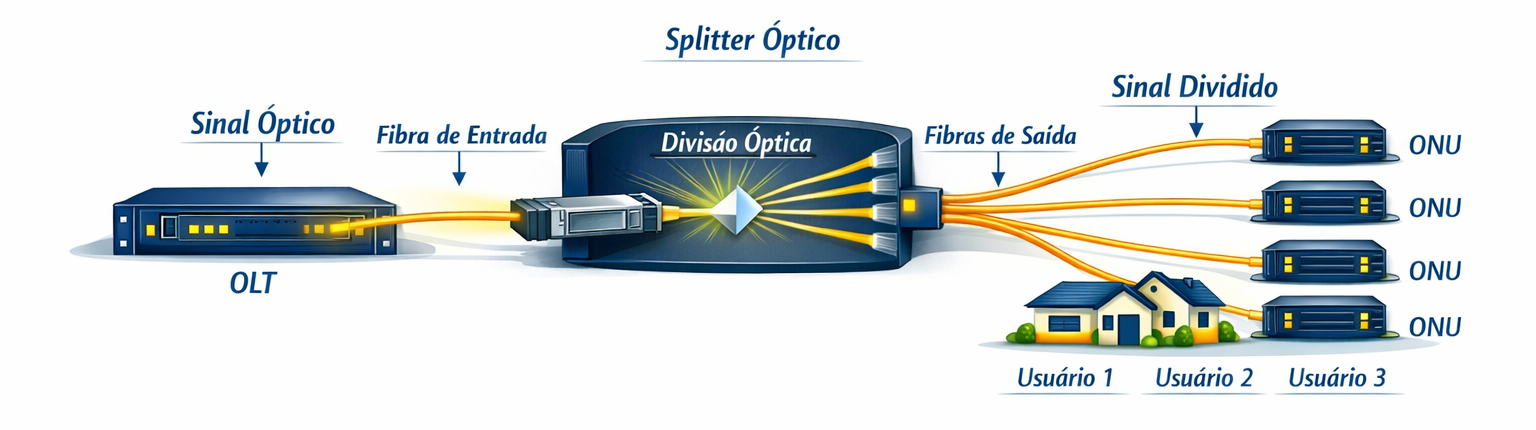
\includegraphics[width=\textwidth]{images/splitter_optico.png}
		\par\footnotesize Fonte: Elaboração própria com auxílio de \gls{ia}.
    }
\end{figure}

Entre os componentes passivos, os \textit{splitters} geralmente representam a maior parcela da atenuação em redes \gls{pon}, uma vez que realizam a divisão do sinal em múltiplas derivações ao longo da rede de distribuição. Em projetos \gls{ftth}, a perda introduzida por esses componentes tende a superar as perdas associadas a conectores e emendas, tornando-se um fator determinante no dimensionamento do enlace \cite{keiser2011pon,apnic_gpon_budget}.

A perda na inserção de um \textit{splitter} está diretamente relacionada à sua razão de derivação. Em configurações balanceadas, o sinal é distribuído de forma uniforme entre todas as saídas, resultando em perdas semelhantes em cada ramificação. Já em configurações desbalanceadas, a divisão ocorre de forma assimétrica, permitindo priorizar determinados caminhos da rede, porém introduzindo níveis distintos de atenuação entre as saídas, o que exige uma análise individualizada do orçamento para cada ramificação final \cite{keiser2011pon}.

A Tabela~\ref{tab:perdas_splitters} apresenta valores típicos de perda de inserção para diferentes configurações de \textit{splitters}, incluindo divisões balanceadas e desbalanceadas, amplamente utilizadas como referência no planejamento de redes \gls{pon} \cite{apnic_gpon_budget,holight_optical_budget}.

\begin{table}[ht!]
\centering
\caption{Perdas típicas de inserção de \textit{splitters} ópticos em redes \gls{pon}}
\label{tab:perdas_splitters}
\begin{tabular}{c c c}
\hline
\textbf{Splitter} & \textbf{Tipo de divisão} & \textbf{Perda típica (dB)} \\
\hline
1$\times$2   & Balanceada     & 3,5 \\
1$\times$4   & Balanceada     & 7,2 \\
1$\times$8   & Balanceada     & 10,5 \\
1$\times$16  & Balanceada     & 13,7 \\
\hline
10/90 & Desbalanceada & $\approx$ 10,5 / 1,5 \\
20/80 & Desbalanceada & $\approx$ 7,8 / 3,8 \\
30/70 & Desbalanceada & $\approx$ 6,3 / 5,5 \\
40/60 & Desbalanceada & $\approx$ 4,7 / 6,8 \\
\hline
\end{tabular}
\end{table} 

Os valores apresentados na Tabela~\ref{tab:perdas_splitters} representam perdas típicas utilizadas como referência no planejamento de redes \gls{ftth}. Em especial, os \textit{splitters} desbalanceados introduzem níveis distintos de atenuação entre as saídas, o que permite flexibilizar o projeto da rede, mas exige que o orçamento seja calculado individualmente para cada ramal. Assim, a correta modelagem das perdas associadas aos \textit{splitters} é fundamental para garantir que todos os enlaces atendam aos limiares de sensibilidade estabelecidos para os terminais ativos do projeto.

\subsection{Perdas Concentradas: Conectores e Emendas}

Além da atenuação distribuída ao longo do meio físico, o orçamento óptico em redes \gls{pon} é influenciado por perdas concentradas introduzidas por conexões e emendas, conforme ilustrado na Figura~\ref{fig:perdas_conexoes_emendas}. Cada conector  presente na \gls{olt}, nas caixas de terminação e nas \glspl{onu} contribui com perdas adicionais, tipicamente na faixa de 0,2 a 0,5~dB, enquanto as emendas por fusão inseridas ao longo da fibra apresentam atenuações menores individualmente, porém relevantes quando acumuladas. 

\begin{figure}[ht!]
	\caption{Perdas introduzidas por conexões e emendas na rede \gls{pon}}
	\label{fig:perdas_conexoes_emendas}
    \centering
    \parbox{16cm}{
		\centering
		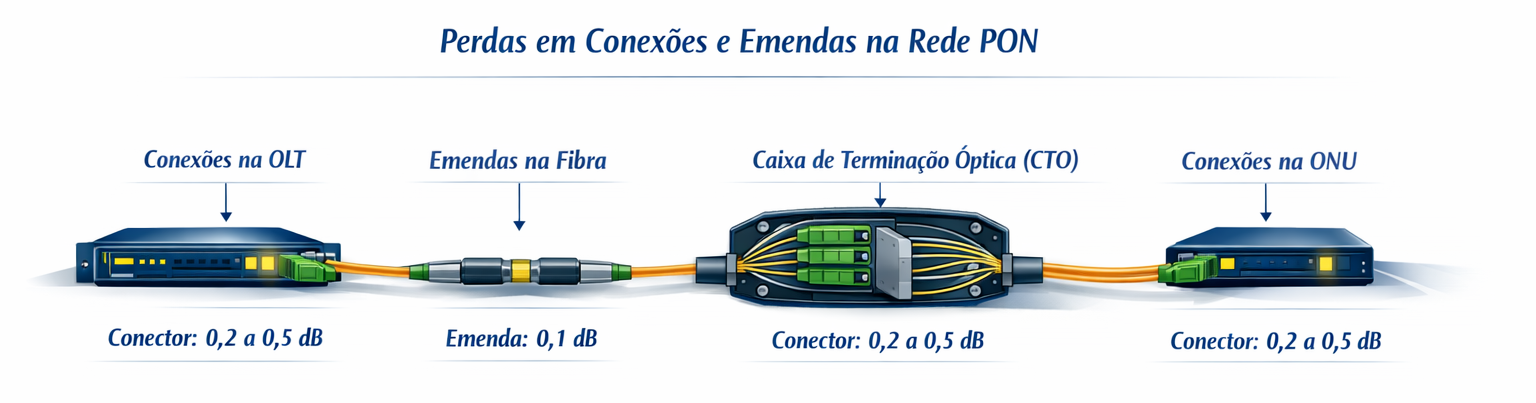
\includegraphics[width=\textwidth]{images/perdas_conexoes_emendas.png}
		\par\footnotesize Fonte: Elaboração própria com auxílio de \gls{ia}.
    }
\end{figure}

Dessa forma, a quantidade de interconexões e fusões realizadas em campo passa a ser um fator importante na previsão de desempenho do canal, reforçando a necessidade de planejamento criterioso da infraestrutura de distribuição. Além das perdas introduzidas pelos componentes passivos ao longo do trajeto, a viabilidade do projeto também depende diretamente das características dos equipamentos utilizados, em especial da potência de transmissão e da sensibilidade de recepção dos transceptores instalados na \gls{olt} e nas \gls{onu}.

A análise do orçamento óptico, embora fundamentada em princípios bem estabelecidos, envolve a consideração simultânea de diversos parâmetros técnicos e da interação entre múltiplos elementos ao longo do enlace. Em projetos reais de sistemas \gls{pon}, especialmente em implantações \gls{ftth} de maior escala, a quantidade de componentes, variações topológicas e diferentes cenários de expansão tornam esse processo progressivamente mais complexo. Nesse contexto, a forma como essa margem de transmissão é calculada, documentada e validada passa a exercer influência direta sobre a confiabilidade do projeto, motivando o uso de ferramentas e métodos específicos para apoiar o planejamento dessas redes.

\section{Ferramentas e Métodos Atuais de Planejamento}

O planejamento de redes ópticas \gls{pon} é atualmente realizado com o auxílio de diferentes ferramentas e métodos, que variam desde abordagens essencialmente manuais até soluções computacionais mais especializadas. Em geral, esses recursos são empregados para estimar o orçamento de potência, definir a topologia física e organizar a distribuição dos componentes ao longo do enlace. Apesar de contribuírem para o processo de projeto, muitas dessas abordagens apresentam limitações relacionadas à integração entre cálculo técnico e representação visual da rede, à flexibilidade na modelagem da topologia e à dependência de intervenções manuais, fatores que podem comprometer a eficiência do dimensionamento de sistemas \gls{ftth} \cite{keiser2011pon,munzner2014visualization}. 

Uma prática amplamente adotada no planejamento de redes \gls{pon} consiste na utilização de planilhas eletrônicas para o cálculo do orçamento. Nessas planilhas, são inseridos manualmente parâmetros como distâncias de fibra, perdas associadas a conectores, fusões e dispositivos passivos, bem como margens de segurança definidas pelo projetista. Embora essa abordagem viabilize as estimativas necessárias, ela depende fortemente da correta inserção dos dados e da interpretação manual dos resultados, o que torna o processo suscetível a inconsistências, especialmente em projetos com múltiplos componentes distribuídos geograficamente \cite{keiser2011pon}. 

Além das planilhas, o planejamento da topologia da rede é frequentemente realizado por meio de diagramas manuais ou ferramentas genéricas de desenho, que auxiliam a organização dos elementos e suas interconexões. Esse tipo de representação costuma não estar integrado ao cálculo, exigindo manutenção paralela entre documentação visual e planilhas de perdas, o que tende a aumentar retrabalho quando a topologia sofre alterações ao longo do projeto.

Paralelamente, observa-se o uso de soluções de georreferenciamento (\gls{gis}) para o planejamento e, principalmente, para a documentação e operação de redes \gls{ftth}. Estudos e relatos técnicos descrevem abordagens nas quais o \gls{gis} é empregado para mapear rotas, distribuir elementos, além de manter registros georreferenciados da infraestrutura instalada, favorecendo documentação e gestão operacional \cite{chakali2025gis_ftth,vargas2025gis_ecuador,irjet2017ftth_gis_autocad,qgis2016ftth_case}. Esse enfoque é particularmente útil para inventário e manutenção, pois consolida a localização física de cabos, caixas, rotas e pontos de acesso em um ambiente espacial.

Entretanto, do ponto de vista da compreensão lógica da rede \gls{pon}, é comum que soluções orientadas ao registro geográfico privilegiem a representação dos ativos a partir do mapa e do cadastro de componentes (cabos, caixas, \textit{splitters} e fusões), com navegação por camadas e consultas por localização \cite{chakali2025gis_ftth,vargas2025gis_ecuador}. Nessa perspectiva, a visualização pode enfatizar ``onde'' os elementos estão e ``o que'' está cadastrado, mas nem sempre favorece uma leitura lógica integrada do encadeamento completo da rede, desde a \gls{olt} até os pontos finais de atendimento, especialmente quando o usuário precisa compreender rapidamente as ligações entre os elementos em diferentes níveis da topologia.

Em alguns sistemas de inventário, a própria documentação do fabricante descreve a existência de representações de rede que combinam inventário físico e lógico e permitem a análise de circuitos e topologias, indicando que o tema de integração entre camadas é relevante na prática \cite{servicenow_inventory_2024}. Ainda assim, quando a visualização permanece predominantemente geográfica, tende a ser mais comum a inspeção de elementos por localidade (por exemplo, detalhes de caixas, emendas e terminais acessados a partir do mapa) do que uma representação lógica global de todas as conexões \gls{pon} de ponta a ponta.

De modo geral, a fragmentação entre cálculo, documentação geográfica e representação lógica pode dificultar a identificação de inconsistências e a análise do impacto de alterações na topologia. Nesse contexto, torna-se relevante considerar abordagens que integrem diferentes etapas do planejamento \cite{munzner2014visualization,keiser2011pon}.

A Figura~\ref{fig:comparacao_planejamento} ilustra essa diferença, comparando o processo manual, caracterizado por etapas independentes e suscetíveis a erros, com o uso de ferramentas integradas, que proporcionam automação, centralização das informações e maior confiabilidade na análise do projeto.

\begin{figure}[htb]
	\caption{Comparação entre o planejamento manual e o uso de ferramentas integradas no projeto de redes ópticas}
	\label{fig:comparacao_planejamento}
    \centering
    \parbox{16cm}{
		\centering
		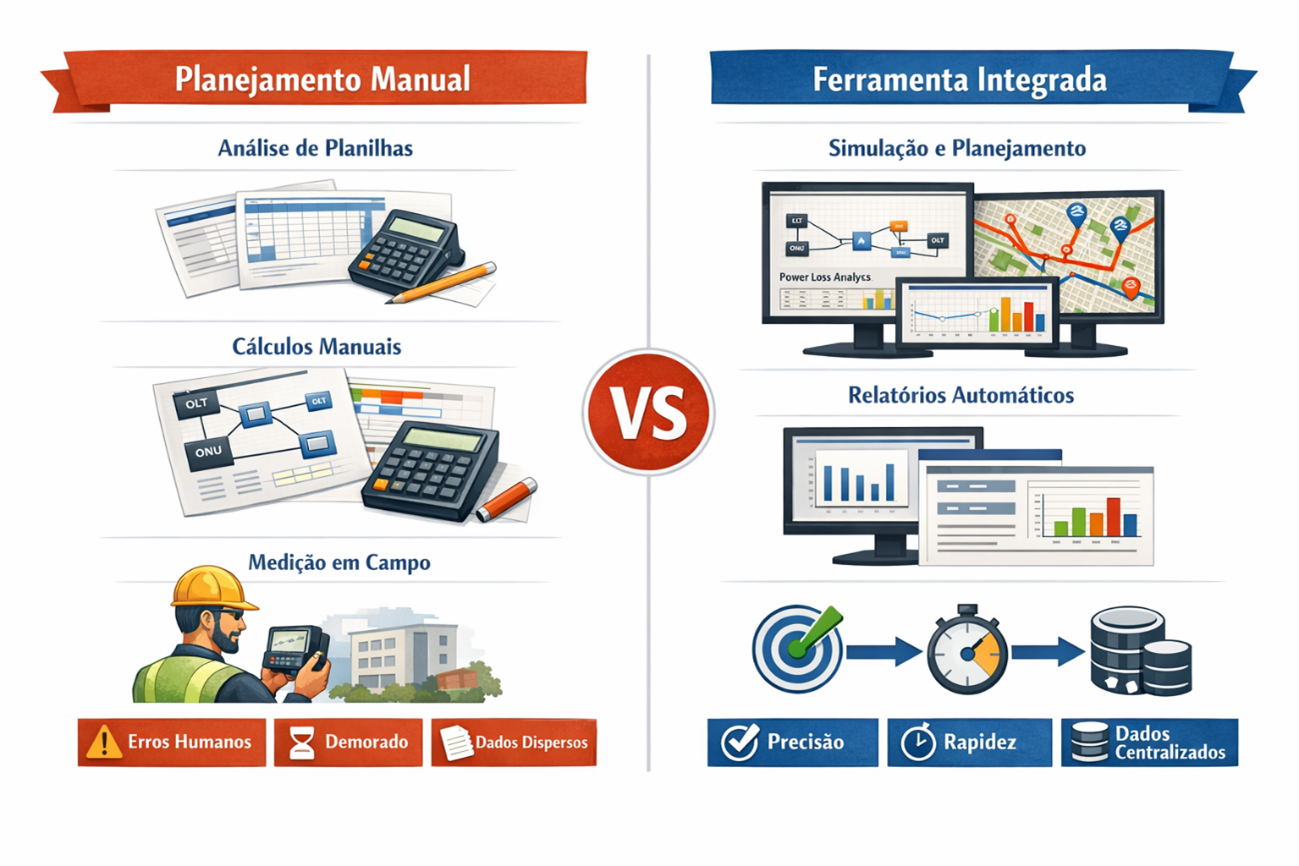
\includegraphics[width=\textwidth]{images/comparacao_planejamento.png}
		\par\footnotesize Fonte: Elaboração própria com auxílio de \gls{ia}.
    }
\end{figure}

\section{Visualização de Dados em Sistemas Complexos}

Sistemas complexos caracterizam-se pela presença de múltiplos elementos interconectados, cujas relações não podem ser plenamente compreendidas por meio da análise isolada de cada componente. Nesses sistemas, o comportamento global emerge a partir da interação entre as partes, tornando a interpretação baseada apenas em dados tabulares ou descrições textuais limitada. Nesse contexto, a visualização de dados assume um papel fundamental como instrumento de apoio à cognição, permitindo transformar informações abstratas em representações que favorecem a compreensão, a análise e a tomada de decisão \cite{card1999information,ware2013information}.

A visualização de dados não se restringe à apresentação estética da informação, mas atua como um meio de ampliar as capacidades cognitivas do usuário. Conforme discutido por \citeonline{card1999information}, representações visuais bem projetadas reduzem a carga cognitiva, facilitam a identificação de padrões e tornam explícitas as relações que seriam difíceis de perceber em formatos tradicionais. Em sistemas com grande volume de dados e múltiplas dependências, como redes de telecomunicações, essa exibição passa a ser um elemento essencial para compreender a estrutura e o funcionamento do sistema como um todo.

\begin{figure}[htb]
	\caption{Processo de visualização de dados em sistemas complexos, desde a coleta e integração de dados até a geração de \textit{insights} para apoio à tomada de decisão}
	\label{fig:visualizacao_sistemas_complexos}
    \centering
    \parbox{16cm}{
		\centering
		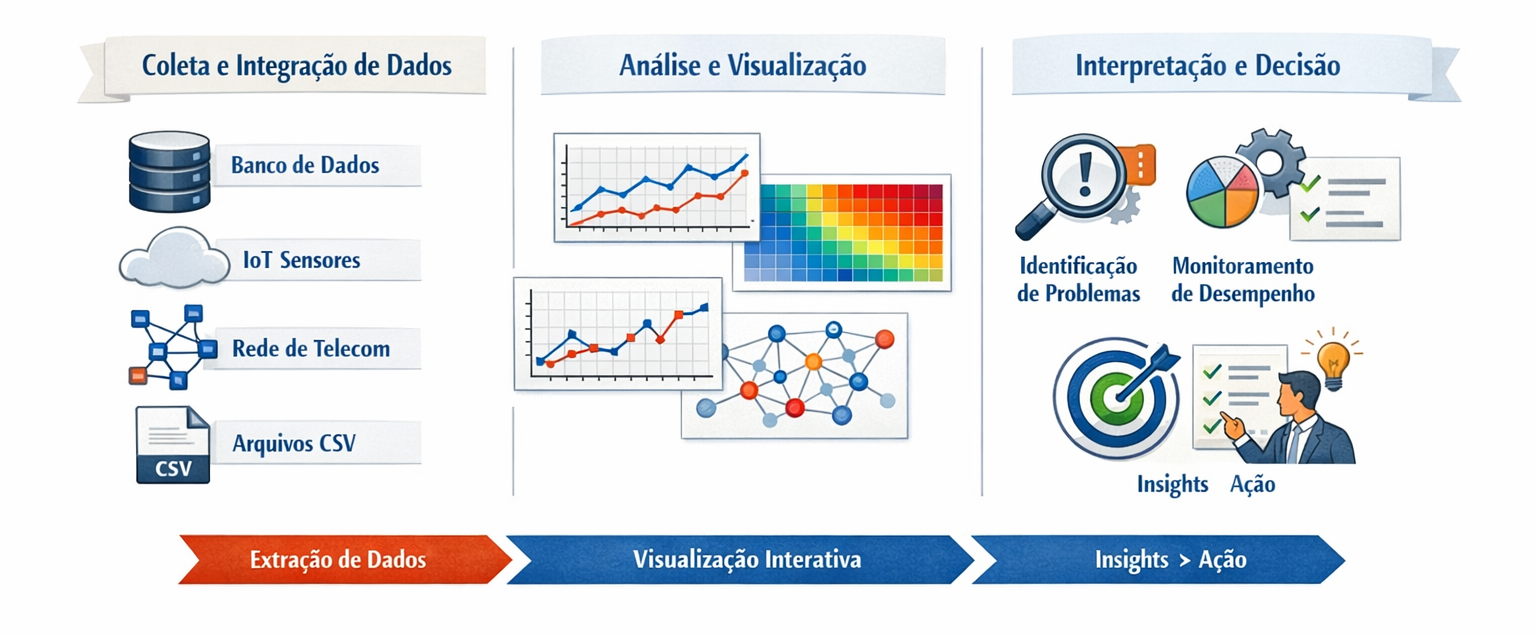
\includegraphics[width=\textwidth]{images/visualizacao_sistemas_complexos.png}
		\par\footnotesize Fonte: Elaboração própria com auxílio de \gls{ia}.
    }
\end{figure}

Conforme ilustrado na Figura~\ref{fig:visualizacao_sistemas_complexos}, o mapeamento de dados em sistemas complexos envolve múltiplas etapas interdependentes, incluindo a coleta e integração de registros provenientes de diferentes fontes, a análise e representação visual dessas informações e, por fim, a interpretação dos resultados para identificação de padrões, geração de \textit{insights} e suporte à tomada de decisão \cite{munzner2014visualization,card1999information}.

Um aspecto particularmente relevante em cenários complexos é a representação de relações, hierarquias e fluxos. Diferentemente de dados independentes, esses casos exigem exibições capazes de evidenciar conexões entre elementos, bem como sua organização em diferentes níveis. Segundo \citeonline{ware2013information}, a percepção humana é especialmente eficiente na identificação de relações espaciais e estruturais quando estas são apresentadas de forma gráfica, o que reforça a importância de representações visuais para o entendimento de topologias e interdependências.

A interatividade constitui um fator determinante para a compreensão desses tipos de sistemas. Interfaces interativas permitem que o usuário explore diferentes níveis de detalhe, alterne entre visões globais e locais, e investigue relações específicas conforme sua necessidade. \citeonline{munzner2014visualization} destaca que abordagens interativas, baseadas nos princípios de foco e contexto, são particularmente eficazes para apoiar a análise de sistemas extensos e hierárquicos, nos quais uma única representação estática dificilmente seria suficiente .

No contexto das redes ópticas \gls{pon}, a complexidade decorre não apenas da quantidade de elementos envolvidos, mas também da forma como eles se conectam logicamente ao longo da rede. A topologia \gls{pon} apresenta uma estrutura hierárquica, com divisões sucessivas do sinal e múltiplos caminhos possíveis entre a central e os usuários finais. A compreensão desse encadeamento lógico é dificultada quando a informação é apresentada exclusivamente em tabelas, planilhas ou visualizações fragmentadas, uma vez que essas abordagens não evidenciam de maneira clara as relações entre os componentes.

A aplicação de princípios de \textit{design} gráfico em cenários complexos torna-se particularmente relevante para o planejamento de redes \gls{pon}. Representações visuais que evidenciem a topologia lógica da rede, aliadas à interatividade, permitem ao projetista compreender o conjunto das ligações, identificar dependências críticas e avaliar o impacto de modificações na estrutura da rede. Conforme apontado por \citeonline{few2012information}, visualizações eficazes devem priorizar clareza, consistência e alinhamento com as tarefas cognitivas do usuário, de modo a apoiar a análise e não apenas a apresentação da informação.

Assim, a representação gráfica, quando aplicada de forma adequada, contribui diretamente para a compreensão de sistemas complexos e para a melhoria do processo decisório. No escopo deste trabalho, esses conceitos fundamentam a adoção de uma abordagem que integra cálculo técnico e visualização interativa da topologia lógica da rede \gls{pon}, visando oferecer ao projetista uma visão mais clara, consistente e abrangente do sistema planejado.

\section{Aplicações Web e Arquitetura Cliente-Servidor}
 
Aplicações web são sistemas de software acessados por meio de um navegador e disponibilizados por uma infraestrutura de rede, permitindo centralizar dados e serviços em um ambiente servidor. Em comparação com aplicações locais, esse modelo reduz dependências do dispositivo do usuário e facilita manutenção e atualização, pois evoluções no servidor tornam-se imediatamente disponíveis aos clientes. Do ponto de vista da engenharia de software, a definição de uma arquitetura clara é essencial para favorecer confiabilidade, manutenibilidade e evolução do sistema ao longo do tempo \cite{pressman2014software,sommerville2016software}.

A organização mais comum para esse tipo de sistema é o modelo cliente-servidor, no qual responsabilidades são distribuídas entre o cliente (interface e interação) e o servidor (processamento, regras de negócio e gerenciamento de dados). Essa separação permite que diferentes tecnologias sejam empregadas em cada parte e contribui para modularidade, reutilização e escalabilidade, uma vez que o servidor pode atender múltiplas requisições simultâneas e ter sua capacidade ampliada por ajustes na infraestrutura \cite{tanenbaum2011networks,pressman2014software}.

O modelo cliente-servidor possibilita a separação entre interface, processamento e armazenamento de dados, contribuindo para a modularidade e a escalabilidade do sistema. A Figura~\ref{fig:cliente_servidor} ilustra essa arquitetura, evidenciando o fluxo de comunicação entre as duas partes por meio de requisições e respostas \cite{tanenbaum2011networks,pressman2014software}.

\begin{figure}[htb]
	\caption{Modelo de arquitetura cliente-servidor, destacando a interação entre cliente e servidor por meio de requisições e respostas em uma rede de comunicação}
	\label{fig:cliente_servidor}
    \centering
    \parbox{16cm}{
		\centering
		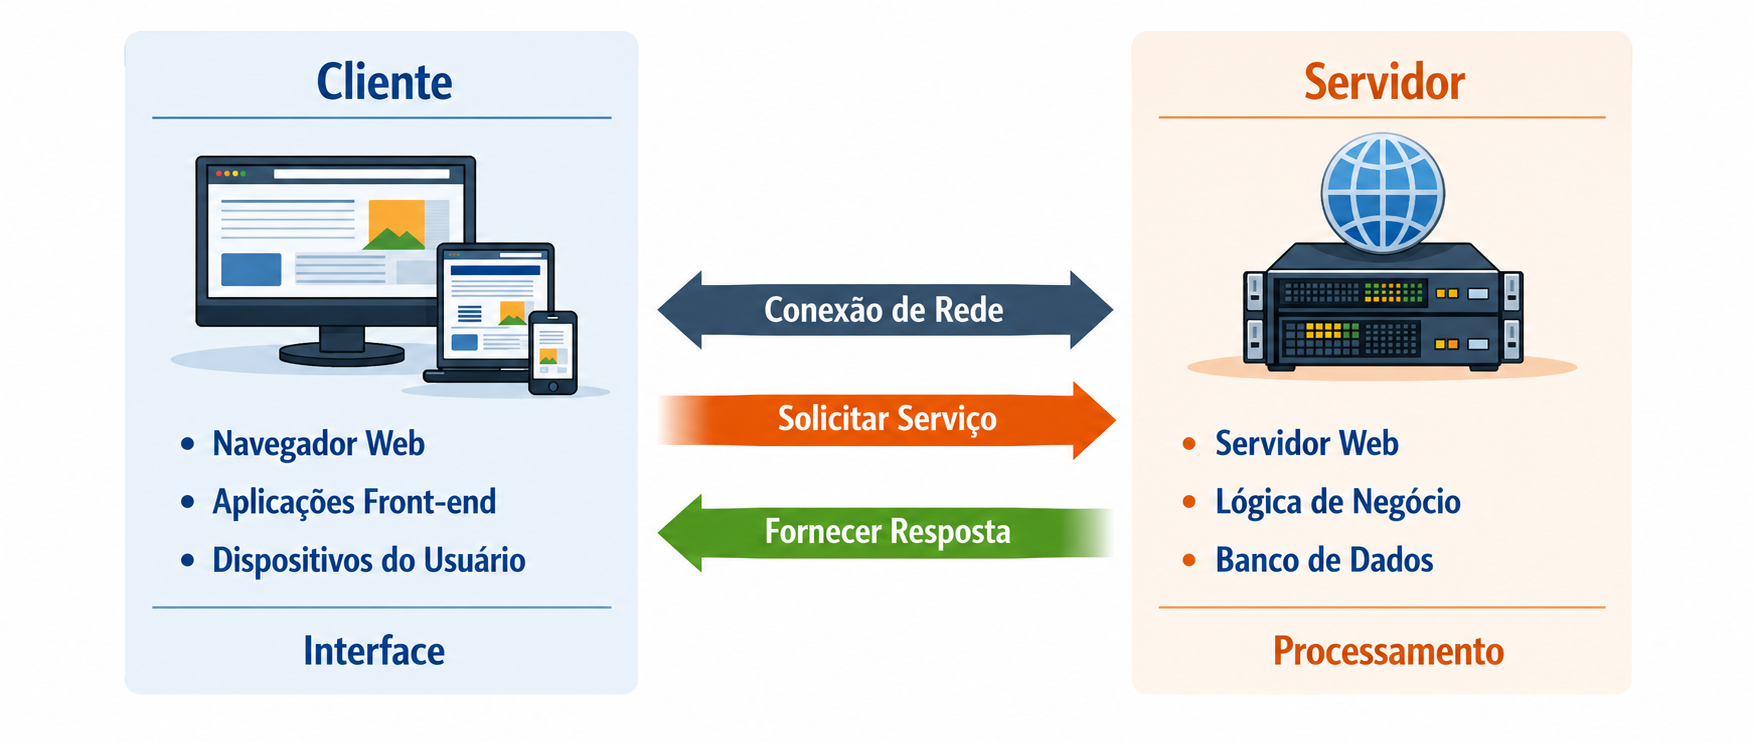
\includegraphics[width=\textwidth]{images/cliente_servidor.png}
		\par\footnotesize Fonte: Elaboração própria com auxílio de \gls{ia}.
    }
\end{figure}

No contexto de aplicações web, essa divisão é frequentemente descrita como \textit{frontend} e \textit{backend}: o \textit{frontend} concentra a camada de apresentação e a experiência do usuário, enquanto o \textit{backend} expõe serviços e recursos e executa validações e operações sobre os dados. Em muitas soluções, essa organização é refinada em uma arquitetura segmentada, separando apresentação, lógica de aplicação e persistência. Ao desacoplar essas responsabilidades, mudanças em um nível tendem a produzir impacto limitado nos demais níveis, reduzindo a complexidade do sistema e facilitando testes, manutenção e atualização \cite{pressman2014software,sommerville2016software}.

A partir dessa base arquitetural, a integração entre cliente e servidor ocorre por meio de interfaces bem definidas (\glspl{api}), usualmente sobre o protocolo \gls{http}, e pode adotar estilos e padrões específicos conforme as necessidades do sistema. Assim, conceitos como \gls{mvc} (para organização interna do \textit{backend}), \gls{rest} (para o estilo de comunicação) e \gls{json} (para representação de dados) complementam o modelo cliente-servidor ao fornecerem mecanismos práticos para estruturar, expor e interoperar funcionalidades e informações em aplicações web distribuídas.

Nesse contexto, a arquitetura cliente-servidor será empregada neste trabalho para estruturar a aplicação web proposta, permitindo separar a interface de modelagem visual da rede das rotinas de cálculo e processamento, favorecendo a organização e a escalabilidade do sistema.

\section{Padrão Arquitetural \gls{mvc}}

O padrão arquitetural \gls{mvc} é amplamente utilizado no desenvolvimento de aplicações como uma forma de organizar o sistema a partir da separação de responsabilidades entre seus componentes. Proposto originalmente por \citeonline{reenskaug1979mvc}, o \gls{mvc} estabelece uma divisão clara entre a representação dos dados, a lógica de controle e a interface com o usuário, contribuindo para a modularidade e a manutenção do software ao longo do tempo.

No padrão \gls{mvc}, o \textit{Model} é responsável pela representação dos dados e pelas regras de negócio da aplicação. Essa camada encapsula a lógica associada ao domínio do problema, incluindo validações, cálculos e estruturas de dados, mantendo-se independente da forma como as informações são apresentadas ao usuário. Essa característica favorece a reutilização e a consistência do comportamento do sistema \cite{pressman2014software}.

A \textit{View} corresponde à camada de apresentação da aplicação, sendo responsável por exibir as informações ao usuário e permitir sua interação com o sistema. No contexto de aplicações web, a \textit{View} é frequentemente implementada por meio de interfaces gráficas executadas no navegador, que consomem dados fornecidos pelos demais componentes do sistema. Ao isolar a apresentação da lógica de negócio, o padrão \gls{mvc} permite que alterações na interface sejam realizadas sem impactar diretamente o processamento interno da aplicação \cite{sommerville2016software}.

O \textit{Controller} atua como intermediário entre o \textit{Model} e a \textit{View}, sendo responsável por receber as requisições do usuário, interpretá-las e acionar as operações apropriadas no \textit{Model}. Após o processamento, o \textit{Controller} coordena a atualização da \textit{View}, garantindo que as informações apresentadas reflitam o estado atual dos dados. Esse papel de mediação contribui para a organização do fluxo de controle da aplicação e para a separação clara das responsabilidades, conforme ilustrado na Figura \ref{fig:mvc} \cite{pressman2014software}.

\begin{figure}[htb]
	\caption{Fluxo de interação do padrão \gls{mvc}}
	\label{fig:mvc}
    \centering
    \parbox{16cm}{
		\centering
		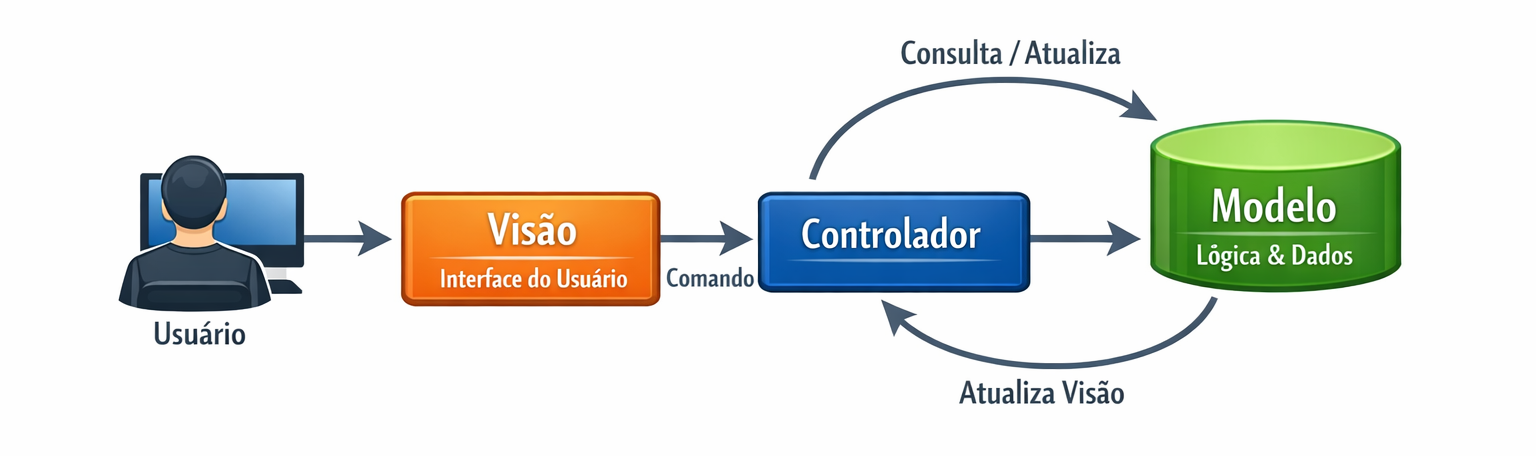
\includegraphics[width=\textwidth]{images/mvc.png}
		\par\footnotesize Fonte: Elaboração própria com auxílio de \gls{ia}.
    }
\end{figure}

\%A utilização do padrão \gls{mvc} em aplicações web favorece a construção de sistemas mais organizados, compreensíveis e extensíveis, especialmente em cenários que envolvem processamento técnico e manipulação de dados estruturados. Ao separar a lógica de negócio da interface e do controle de fluxo, o \gls{mvc} estabelece uma base arquitetural adequada para a integração com outros estilos e tecnologias, como serviços web e interfaces interativas, contribuindo para a evolução consistente da aplicação ao longo do tempo.

Dessa forma, o padrão \gls{mvc} será adotado na organização do \textit{backend} da aplicação, permitindo separar a lógica de cálculo do orçamento óptico, o controle das requisições e a manipulação dos dados, contribuindo para a clareza, manutenção e escalabilidade do sistema desenvolvido.

\section{Comunicação Web: \gls{http} e \glspl{api}}

A comunicação entre componentes em aplicações web baseia-se, de forma predominante, em mecanismos padronizados que permitem a troca de informações entre clientes e servidores distribuídos em rede. No contexto do modelo cliente-servidor, essa comunicação é realizada por meio de protocolos que definem como as requisições são enviadas, como as respostas são estruturadas e como os dados são transmitidos de forma confiável. Entre esses protocolos, destaca-se o \gls{http}, amplamente adotado como base para a comunicação em aplicações web modernas \cite{tanenbaum2011networks}.

O protocolo \gls{http} define um modelo de comunicação do tipo requisição-resposta, no qual o cliente envia uma solicitação ao servidor e aguarda o retorno de uma resposta correspondente. Cada requisição contém informações que identificam o recurso desejado e o tipo de operação a ser realizada, enquanto a resposta do servidor inclui os dados solicitados ou o resultado do processamento, além de códigos de \textit{status} que indicam o sucesso ou falha da comunicação. Esse modelo simples e padronizado contribui para a interoperabilidade entre sistemas heterogêneos e para a ampla adoção do \gls{http} em ambientes distribuídos \cite{tanenbaum2011networks}.

No desenvolvimento de soluções web, o uso do \gls{http} é frequentemente associado ao conceito de \glspl{api}. Uma \gls{api} pode ser entendida como um conjunto de interfaces e regras que permitem a troca de informações entre diferentes componentes de software, definindo como funcionalidades e dados podem ser acessados de forma controlada. Em aplicações baseadas em arquitetura cliente-servidor, as \glspl{api} desempenham papel fundamental ao estabelecer um ponto de comunicação bem definido entre o \textit{frontend} e o \textit{backend}, promovendo o desacoplamento entre a interface do usuário e a lógica de processamento, conforme ilustrado na Figura~\ref{fig:http_api} \cite{sommerville2016software}.

\begin{figure}[htb]
	\caption{Comunicação entre cliente e servidor por meio de \gls{http} e \gls{api}}
	\label{fig:http_api}
    \centering
    \parbox{16cm}{
		\centering
		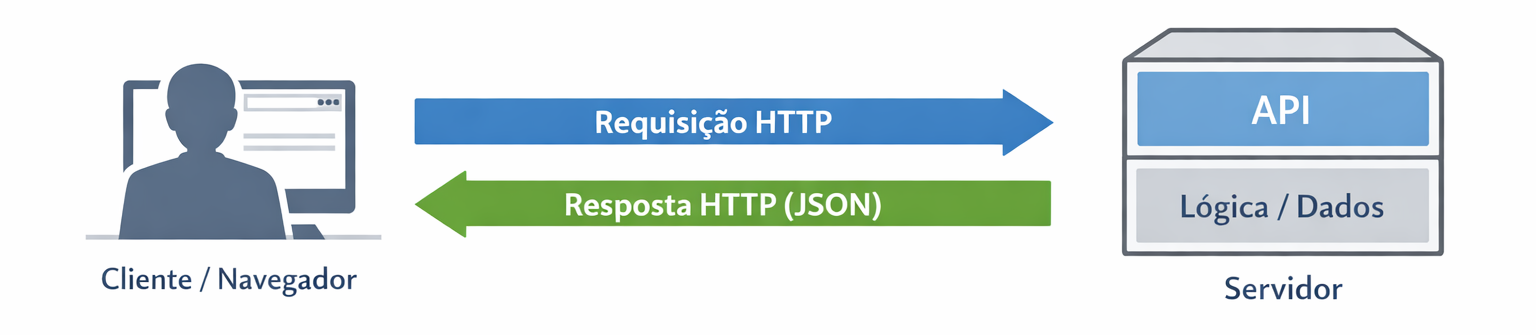
\includegraphics[width=\textwidth]{images/http_api.png}
		\par\footnotesize Fonte: Elaboração própria com auxílio de \gls{ia}.
    }
\end{figure}

A adoção de \glspl{api} na comunicação web contribui para a modularidade e a extensibilidade das aplicações, uma vez que diferentes clientes podem consumir os mesmos serviços oferecidos pelo servidor, desde que respeitem as interfaces estabelecidas. Essa abordagem facilita a evolução do sistema, possibilita a integração com outros serviços e reduz a dependência direta entre os componentes da aplicação. Conforme discutido na literatura de engenharia de software, interfaces bem definidas são essenciais para o desenvolvimento de sistemas distribuídos mais organizados, reutilizáveis e de fácil manutenção \cite{pressman2014software}.

O uso do protocolo \gls{http} em conjunto com \glspl{api} constitui a base da comunicação em aplicações web modernas, permitindo a troca estruturada de informações entre clientes e servidores. Essa combinação estabelece o fundamento sobre o qual estilos arquiteturais específicos de comunicação são construídos, viabilizando a implementação de soluções distribuídas escaláveis e interoperáveis.

Assim, a comunicação via \gls{http} será empregada neste trabalho como base para a troca de dados entre os componentes da aplicação, garantindo a interoperabilidade entre a interface web e os serviços responsáveis pelo processamento dos cálculos.


\section{\gls{api} \textit{RESTful}}

O estilo arquitetural \gls{rest} foi proposto por \citeonline{fielding2000rest} como um conjunto de princípios para a construção de sistemas distribuídos baseados em rede, com foco em escalabilidade, simplicidade e baixo acoplamento entre os componentes. No contexto das aplicações web, o \gls{rest} consolidou-se como uma abordagem amplamente adotada para o desenvolvimento de \glspl{api}, sendo utilizado como base para a comunicação entre clientes e servidores em sistemas cliente-servidor modernos.

Uma \gls{api} \textit{RESTful} organiza a comunicação em torno do conceito de recursos, que representam entidades ou conjuntos de dados manipulados pelo sistema. Cada recurso é identificado de forma única por meio de uma \gls{uri} e pode ser acessado ou manipulado por operações padronizadas. Essas operações são realizadas utilizando os métodos definidos pelo protocolo \gls{http}, o que permite explorar mecanismos amplamente suportados pela infraestrutura da web \cite{fielding2000rest}

Entre os princípios fundamentais do \gls{rest} destaca-se a característica \textit{stateless}, segundo a qual cada requisição enviada pelo cliente ao servidor deve conter todas as informações necessárias para seu processamento. O servidor não mantém estado da sessão do cliente entre requisições, o que contribui para a escalabilidade do sistema e simplifica o gerenciamento das interações. Essa abordagem reduz dependências entre requisições consecutivas e facilita a distribuição da carga de processamento entre diferentes instâncias servidoras, conforme ilustrado na Figura~\ref{fig:api_restfull} \cite{fielding2000rest}.

\begin{figure}[htb]
	\caption{Estrutura conceitual de uma \gls{api} \textit{RESTful}}
	\label{fig:api_restfull}
    \centering
    \parbox{16cm}{
		\centering
		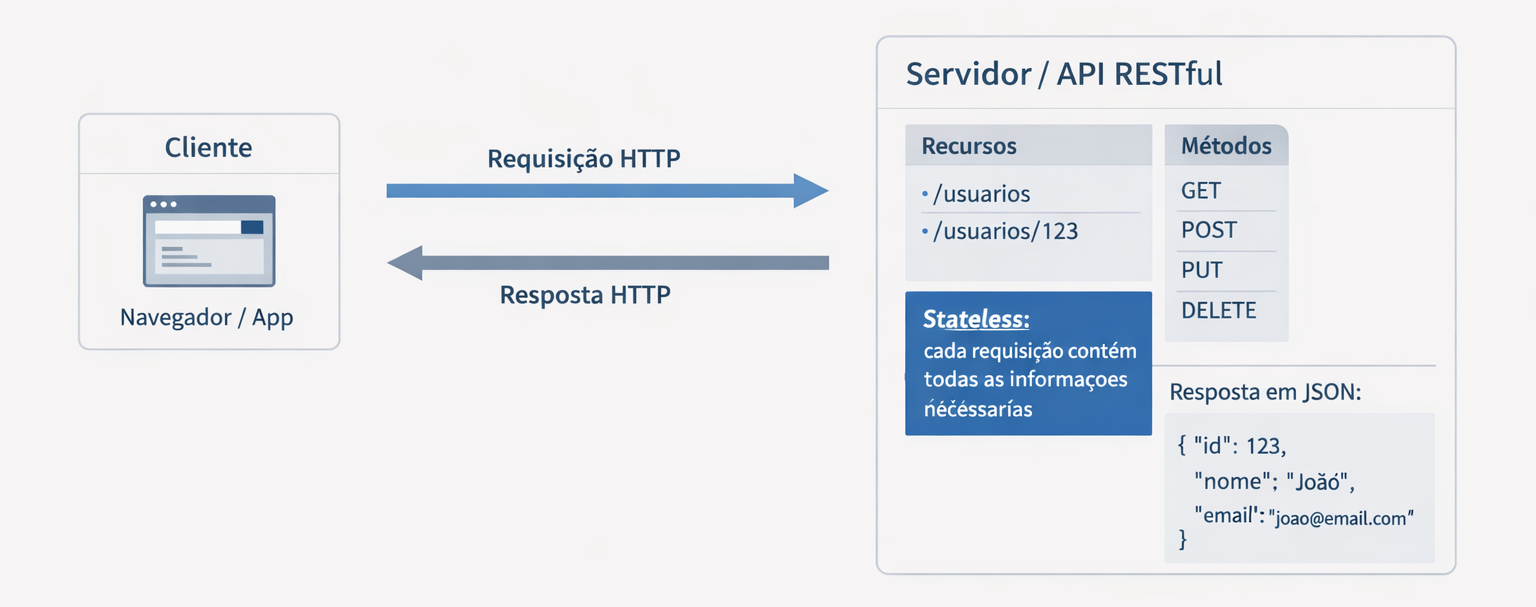
\includegraphics[width=\textwidth]{images/api_restfull.png}
		\par\footnotesize Fonte: Elaboração própria com auxílio de \gls{ia}.
    }
\end{figure}

A adoção do estilo \gls{rest} em aplicações web contribui para a construção de sistemas mais organizados, interoperáveis e extensíveis. Ao basearem a comunicação em princípios bem definidos e amplamente aceitos, as \glspl{api} \textit{RESTful} estabelecem uma infraestrutura de comunicação adequada para aplicações distribuídas que demandam integração entre múltiplos componentes, servindo como base para o intercâmbio estruturado de dados e para a implementação de serviços web modernos \cite{fielding2000rest}.

Nesse contexto, a adoção de uma \gls{api} \textit{RESTful} neste projeto permite estruturar a comunicação entre o \textit{frontend} e o \textit{backend} de forma modular e padronizada, facilitando o envio de dados da topologia da rede e o retorno dos resultados do cálculo do orçamento óptico.

\section{Formato de Intercâmbio de Dados: \gls{json}}

Em aplicações web modernas, a troca de informações entre cliente e servidor requer o uso de formatos de dados padronizados, capazes de representar estruturas de informação de forma clara, eficiente e independente de plataforma. No contexto de \gls{api} \textit{RESTful}, esses formatos desempenham papel essencial, pois viabilizam o intercâmbio estruturado de dados entre diferentes componentes do sistema, garantindo interoperabilidade e consistência na comunicação.

O \gls{json} é um formato leve de representação de dados, baseado em texto, amplamente utilizado em aplicações web e serviços baseados em \gls{http}. Definido originalmente como uma notação derivada da linguagem JavaScript, o \gls{json} consolidou-se como um formato independente de linguagem, sendo suportado por diversas plataformas e ambientes de desenvolvimento. Sua estrutura baseia-se em pares chave-valor e em listas ordenadas, permitindo a representação de dados simples e complexos de maneira hierárquica e legível, conforme ilustrado na Figura~\ref{fig:json_estrutura} \cite{bray2017json}.

\begin{figure}[htb]
	\caption{Estrutura conceitual do formato \gls{json}}
	\label{fig:json_estrutura}
    \centering
    \parbox{16cm}{
		\centering
		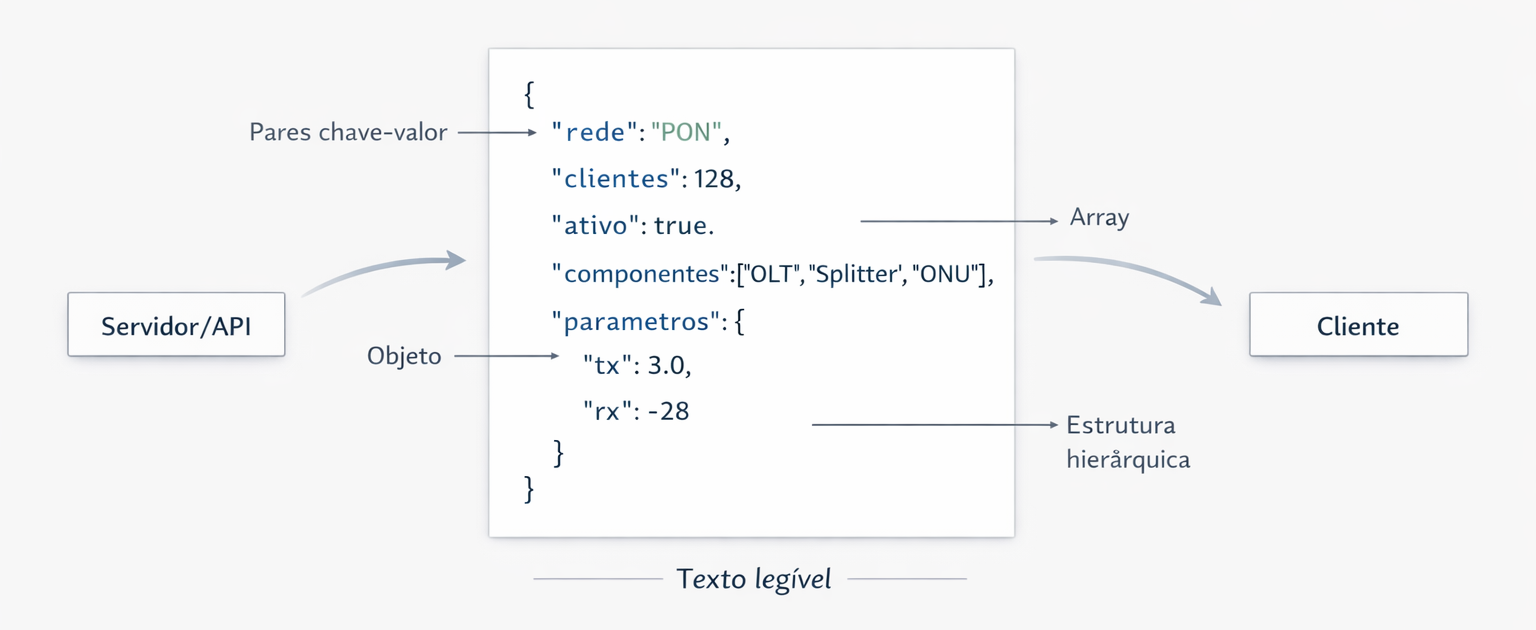
\includegraphics[width=\textwidth]{images/json_estrutura.png}
		\par\footnotesize Fonte: Elaboração própria com auxílio de \gls{ia}.
    }
\end{figure}

Uma das principais características do \gls{json} é sua simplicidade sintática, que facilita tanto a leitura humana quanto o processamento automático pelos sistemas. Em comparação com formatos mais verbosos, como XML, o \gls{json} apresenta menor sobrecarga de dados, contribuindo para a redução do volume de informações enviadas pela rede e para a melhoria do desempenho das aplicações distribuídas. Essas características tornam o \gls{json} particularmente adequado para a comunicação em \glspl{api} \textit{RESTful}, nas quais eficiência e clareza na troca de dados são requisitos relevantes \cite{bray2017json}.

No contexto da arquitetura cliente-servidor, o uso do \gls{json} como formato de intercâmbio assegura a neutralidade tecnológica na transmissão, uma vez que os dados terão representação neutra, independente das tecnologias utilizadas em cada componente. Dessa forma, o servidor pode fornecer informações estruturadas por meio de respostas \gls{http}, enquanto o cliente interpreta e utiliza esses dados conforme suas necessidades de apresentação ou interação, sem dependência direta da implementação interna do servidor \cite{sommerville2016software}.

Além de seu uso na comunicação entre componentes, o \gls{json} também é amplamente empregado para o armazenamento e a serialização de dados estruturados em aplicações web. Sua flexibilidade permite representar configurações, estados e estruturas complexas de informação de forma organizada e facilmente manipulável. Assim, o \gls{json} estabelece-se como um elemento fundamental na infraestrutura de aplicações web modernas, servindo como base para a troca de dados em sistemas distribuídos e integrados.

Dessa forma, o formato \gls{json} será utilizado neste trabalho para representar a topologia da rede óptica, permitindo o armazenamento estruturado dos elementos e sua fácil integração com a visualização interativa implementada com a biblioteca D3.js.

\section{Visualização de Dados em Aplicações Web}

A visualização de dados constitui um elemento fundamental em sistemas computacionais que lidam com grandes volumes de informações ou com estruturas de dados complexas. Seu objetivo principal é transformar dados abstratos em representações visuais que facilitem a compreensão, a análise e a interpretação das informações, apoiando processos de tomada de decisão. Em aplicações web, a visualização assume papel ainda mais relevante, uma vez que a interface gráfica representa o principal meio de interação entre o usuário e os dados processados pelo sistema \cite{card1999information,ware2013information}.

Em sistemas baseados em arquitetura cliente-servidor, a visualização de dados está geralmente associada à camada de apresentação da aplicação, sendo responsável por representar, de forma gráfica, as informações fornecidas pelo \textit{backend}. Essa separação permite que o processamento e a organização dos dados ocorram no servidor, enquanto o cliente se encarrega de exibir essas informações de maneira adequada ao usuário. A utilização de visualizações gráficas contribui para reduzir a carga cognitiva associada à interpretação de dados complexos, tornando explícitas relações, hierarquias e padrões que seriam difíceis de identificar por meio de representações puramente textuais ou tabulares \cite{card1999information}.

As aplicações web modernas demandam visualizações que vão além da simples apresentação estática de informações. A interatividade passou a ser um requisito importante, permitindo que o usuário explore os dados, alterne entre diferentes níveis de detalhe e observe o impacto de modificações nos parâmetros de entrada. Conforme discutido na literatura, visualizações interativas ampliam a capacidade de análise ao combinar representações gráficas com mecanismos de exploração, favorecendo a compreensão de sistemas complexos e dinâmicos, conforme ilustrado na Figura~\ref{fig:visualizacao_web} \cite{munzner2014visualization}.

\begin{figure}[htb]
	\caption{Visualização interativa de dados em aplicações web}
	\label{fig:visualizacao_web}
    \centering
    \parbox{16cm}{
		\centering
		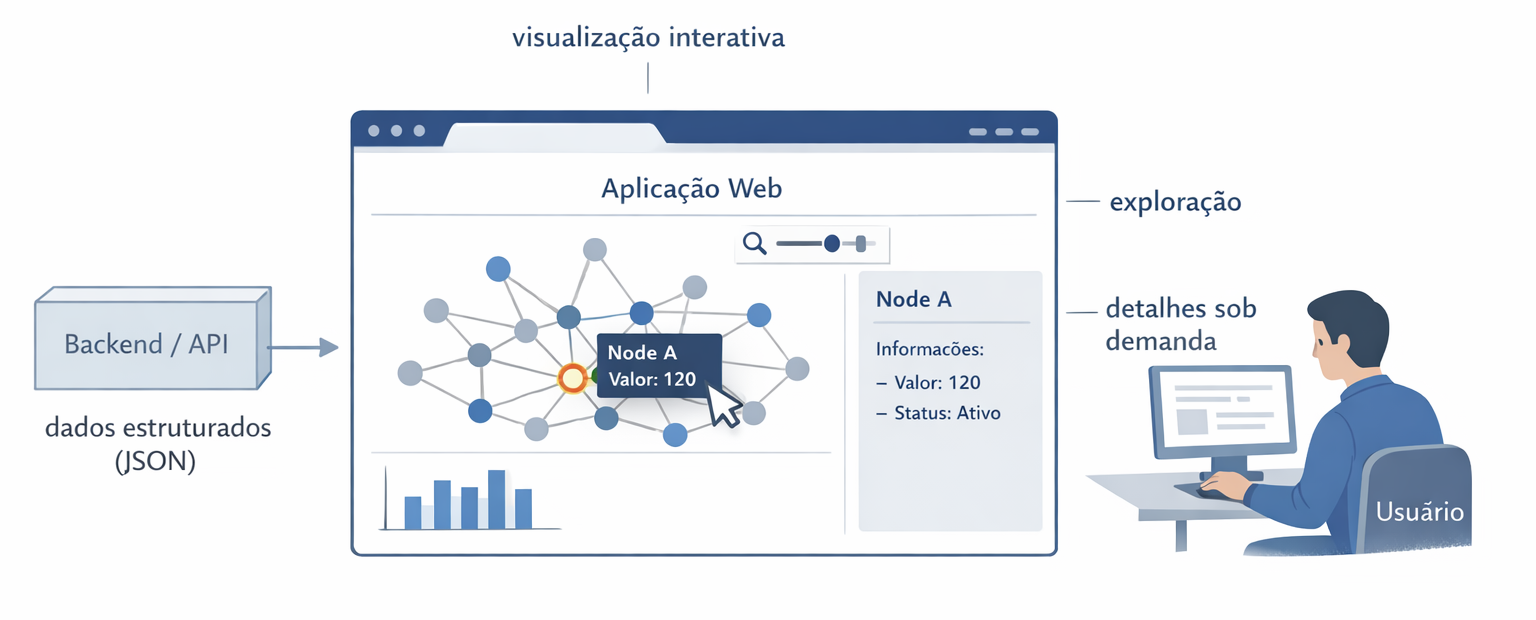
\includegraphics[width=\textwidth]{images/visualizacao_web.png}
		\par\footnotesize Fonte: Elaboração própria com auxílio de \gls{ia}.
    }
\end{figure}

Outro aspecto relevante da visualização de dados em aplicações web é sua integração com dados estruturados provenientes de \glspl{api} e serviços distribuídos. Formatos de intercâmbio como o \gls{json} permitem que informações organizadas sejam transmitidas do servidor para o cliente, onde podem ser processadas e representadas visualmente de forma dinâmica. Essa integração entre dados estruturados e visualização gráfica reforça o papel da visualização como componente essencial na construção de aplicações web voltadas à análise e ao planejamento \cite{sommerville2016software}.

Dessa forma, a visualização de dados em aplicações web constitui um recurso indispensável para a representação clara e eficiente de informações técnicas e estruturadas. Ao permitir a exploração visual dos dados e a interação direta do usuário com as informações apresentadas, as visualizações contribuem para a compreensão global do sistema e para a melhoria da experiência de uso, estabelecendo a base conceitual para o emprego de bibliotecas especializadas em visualização gráfica no ambiente web.

\section{Biblioteca D3.js para Visualização Interativa}

No contexto das aplicações web, a implementação de visualizações interativas demanda o uso de bibliotecas especializadas capazes de transformar dados estruturados em representações gráficas dinâmicas. Entre as ferramentas disponíveis para esse fim, destaca-se a biblioteca D3.js (\textit{Data-Driven Documents}), amplamente utilizada para a criação de visualizações personalizadas e orientadas a dados no ambiente web \cite{bostock2011d3}.

A D3.js baseia-se no princípio de vincular dados diretamente aos elementos do documento, permitindo que mudanças nos dados sejam refletidas automaticamente na representação visual. Essa abordagem orientada a dados possibilita a construção de visualizações altamente flexíveis, nas quais atributos gráficos como posição, cor, forma e tamanho podem ser definidos a partir dos valores dos dados subjacentes. Diferentemente de bibliotecas que oferecem apenas componentes gráficos pré-definidos, a D3.js fornece mecanismos de baixo nível que permitem maior controle sobre a estrutura e o comportamento das visualizações, conforme ilustrado na Figura~\ref{fig:d3js_conceito} \cite{bostock2011d3}.

\begin{figure}[htb]
	\caption{Transformação de dados em elementos visuais interativos com D3.js}
	\label{fig:d3js_conceito}
    \centering
    \parbox{16cm}{
		\centering
		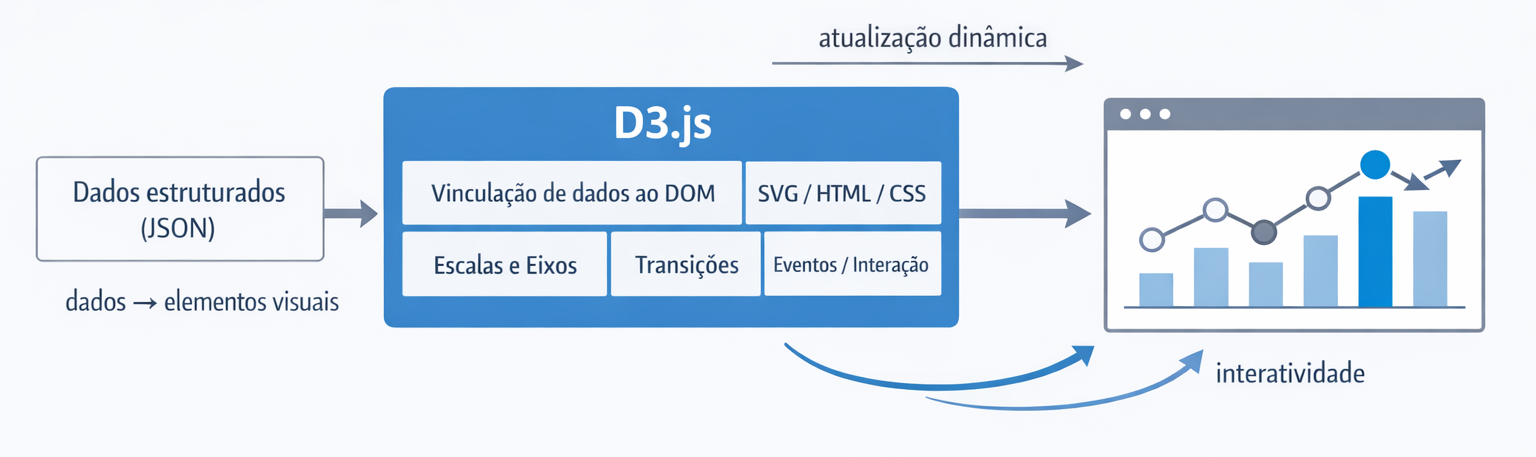
\includegraphics[width=\textwidth]{images/d3js_conceito.png}
		\par\footnotesize Fonte: Elaboração própria com auxílio de \gls{ia}.
    }
\end{figure}

Outro aspecto relevante da D3.js é sua integração nativa com tecnologias fundamentais da web, como \gls{html}, \gls{svg} e \gls{css}. Essa integração permite que as visualizações façam parte da estrutura do documento web, favorecendo a criação de interfaces ricas e interativas sem a necessidade de ambientes gráficos proprietários ou extensões específicas. Além disso, a utilização de padrões abertos contribui para a portabilidade e a compatibilidade das visualizações em diferentes navegadores e dispositivos \cite{bostock2011d3}.

A D3.js também oferece suporte à interatividade, possibilitando a implementação de mecanismos como atualização dinâmica dos dados, animações, transições e respostas a eventos de interação do usuário. Esses recursos são particularmente importantes em aplicações que envolvem a exploração de dados complexos, pois permitem que o usuário investigue diferentes aspectos da informação apresentada, altere parâmetros e observe, em tempo real, os efeitos dessas alterações sobre a visualização \cite{munzner2014visualization}.

A adoção da biblioteca D3.js em aplicações voltadas à visualização de dados proporciona uma base adequada para a representação gráfica interativa de informações técnicas e estruturadas. Ao combinar flexibilidade, integração com padrões web e suporte à interatividade, a D3.js constitui uma ferramenta apropriada para a construção de visualizações que auxiliam na compreensão e na análise de sistemas complexos, especialmente em contextos que demandam clareza na representação da estrutura e do comportamento dos dados.

Nesse sentido, a biblioteca D3.js será utilizada neste projeto para a construção da visualização interativa da topologia da rede, permitindo representar graficamente os elementos e suas conexões, além de atualizar dinamicamente os resultados do orçamento óptico conforme as alterações realizadas pelo usuário.


\section{Execução e Implantação de Aplicações Web (\textit{Docker})}

A execução e a implantação de aplicações web envolvem a definição de um ambiente computacional capaz de suportar corretamente os componentes do sistema, incluindo dependências de software, bibliotecas e configurações necessárias para seu funcionamento. Em aplicações distribuídas, diferenças entre ambientes de desenvolvimento, teste e produção podem introduzir inconsistências que afetam a confiabilidade e a reprodutibilidade do sistema. Nesse contexto, abordagens que visam padronizar o ambiente de execução tornam-se relevantes para a estabilidade e a manutenção das aplicações web.

A conteinerização surge como uma solução para esse problema ao permitir o empacotamento da aplicação e de todas as suas dependências em unidades isoladas, conhecidas como contêineres. Diferentemente de abordagens baseadas em virtualização completa, os contêineres compartilham o núcleo do sistema operacional hospedeiro, oferecendo um ambiente leve e eficiente para a execução de aplicações. Essa característica contribui para a portabilidade do sistema, possibilitando que a aplicação seja executada de forma consistente em diferentes plataformas e infraestruturas \cite{pahl2015containerization}.

O \textit{Docker} é uma das ferramentas mais difundidas para a implementação do modelo de conteinerização, sendo amplamente adotado no desenvolvimento e na implantação de aplicações web. Por meio do \textit{Docker}, torna-se possível definir ambientes de execução padronizados, nos quais a aplicação e seus serviços associados operam de maneira isolada do sistema hospedeiro. Essa padronização reduz dependências externas, simplifica o processo de execução e facilita a replicação do ambiente em diferentes contextos, conforme ilustrado na Figura~\ref{fig:docker_implantacao} \cite{merkel2014docker}.

\begin{figure}[htb]
	\caption{Execução de aplicações web em contêineres \textit{Docker}}
	\label{fig:docker_implantacao}
    \centering
    \parbox{16cm}{
		\centering
		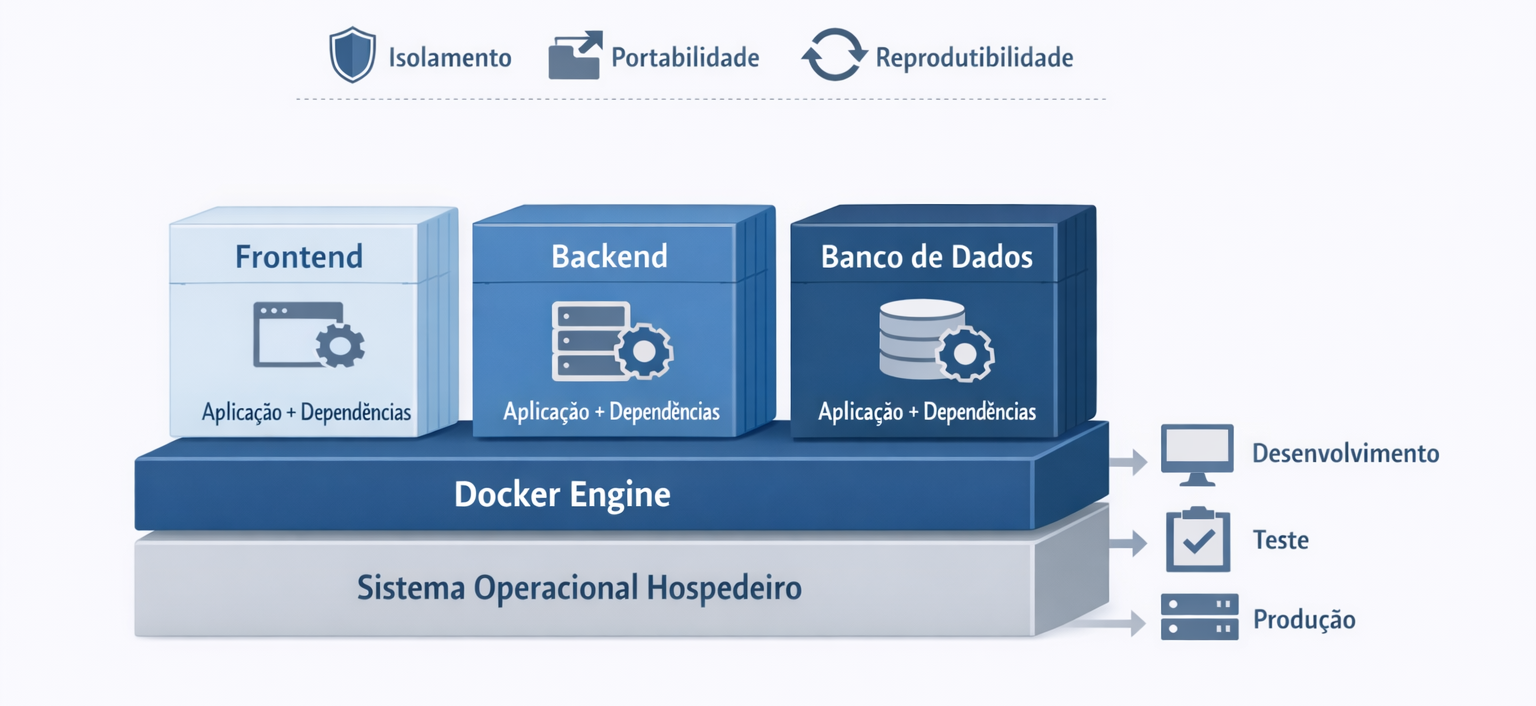
\includegraphics[width=\textwidth]{images/docker_implantacao.png}
		\par\footnotesize Fonte: Elaboração própria com auxílio de \gls{ia}.
    }
\end{figure}

No contexto de aplicações web baseadas em arquitetura cliente-servidor, o uso de contêineres favorece a separação entre os diferentes componentes do sistema, como \textit{frontend} e \textit{backend}, permitindo que cada parte seja executada em um ambiente controlado e consistente. Além disso, a conteinerização contribui para a organização do processo de implantação, uma vez que a aplicação pode ser distribuída e executada de forma uniforme, independentemente do ambiente subjacente.
 
Assim, o \textit{Docker} será utilizado neste trabalho como ferramenta de apoio ao desenvolvimento, permitindo a criação de um ambiente de execução padronizado para a aplicação. Essa abordagem garante que as rotinas de cálculo do orçamento óptico e os serviços da \gls{api} possam ser executados de forma consistente em diferentes ambientes, além de facilitar a posterior implantação do sistema.

\chapter{Metodologia}

Este capítulo apresenta a metodologia adotada no desenvolvimento e na validação da aplicação web proposta para o planejamento de redes ópticas \gls{pon}. Inicialmente, são descritas a natureza da pesquisa e a abordagem metodológica do estudo. Em seguida, detalham-se a arquitetura da solução, as tecnologias empregadas, o processo de desenvolvimento do sistema e os procedimentos definidos para sua validação e análise dos resultados.

\section{Caracterização da Pesquisa}

Esta pesquisa caracteriza-se como aplicada, pois busca desenvolver uma solução computacional voltada à resolução de um problema prático no contexto do planejamento de redes ópticas \gls{ftth} baseadas em \gls{pon}. Quanto aos procedimentos, apresenta natureza experimental, uma vez que envolve a implementação de uma aplicação web interativa e sua avaliação em cenários controlados. Em relação aos objetivos, possui caráter exploratório e descritivo, pois investiga de que modo a integração entre modelagem visual da topologia, cálculo automatizado do orçamento óptico e armazenamento estruturado das informações do projeto pode contribuir para tornar o processo de planejamento mais claro, ágil e confiável \cite{gil2008metodos,prodanov2013metodologia}.

Quanto à abordagem metodológica, o estudo adota método misto, com predominância qualitativa e apoio quantitativo. A dimensão qualitativa está associada à análise da adequação da arquitetura proposta, da interface interativa e do fluxo de uso da ferramenta no contexto do planejamento técnico de redes ópticas. Já a dimensão quantitativa concentra-se na etapa de validação, por meio da comparação entre os valores calculados pelo sistema e os resultados esperados para cenários de teste previamente definidos, além da observação de indicadores de consistência funcional e desempenho. Desse modo, o trabalho envolve tanto o desenvolvimento do software quanto a análise de seu comportamento e de sua capacidade de atender aos objetivos técnicos estabelecidos \cite{creswell2014research}.

Em conformidade com as orientações do \gls{mec} e do \gls{cnpq} sobre integridade científica, declara-se o uso de ferramentas de \gls{ia} generativa durante a elaboração deste trabalho. O Microsoft Copilot foi utilizado como apoio à pesquisa bibliográfica, auxiliando na busca de artigos, livros e referências, bem como na revisão textual. As ferramentas Gemini e ChatGPT foram empregadas na elaboração de imagens e diagramas técnicos, enquanto o Grammarly foi utilizado na verificação ortográfica e gramatical do texto. Ressalta-se, contudo, que a responsabilidade pelo conteúdo intelectual do trabalho, pela seleção e validação das referências, pela veracidade dos dados técnicos sobre redes ópticas, pela análise crítica dos resultados e pela redação final permanece integralmente sob a autoria do pesquisador, assegurando a originalidade e a rastreabilidade do processo científico.

\section{Arquitetura da Solução}

O sistema proposto é estruturado segundo uma arquitetura cliente-servidor. Nessa configuração, o \textit{frontend} concentra a interação com o usuário e a representação gráfica da rede \gls{pon}, enquanto o \textit{backend} reúne a lógica de negócio, as validações e a disponibilização dos dados. Essa divisão favorece a separação de responsabilidades, a modularidade do sistema e a evolução independente entre interface e processamento.

A estrutura da aplicação pode ser compreendida a partir de três partes principais. A primeira corresponde à apresentação, implementada em ambiente web, na qual o usuário constrói visualmente a topologia da rede e acompanha os resultados após o recálculo automático provocado por alterações. A segunda refere-se ao processamento, responsável por tratar as operações solicitadas, validar os parâmetros informados e executar as rotinas de cálculo do orçamento óptico com base nos elementos modelados. A terceira diz respeito aos dados, destinados ao armazenamento estruturado das informações do projeto, incluindo topologia, parâmetros técnicos e resultados calculados. Essa arquitetura será complementada por diagramas e fluxos de interação, de modo a explicitar a comunicação entre as partes do sistema e facilitar a compreensão de seu funcionamento.

Na Figura~\ref{fig:arquitetura_solucao}, observa-se a estrutura da aplicação e o fluxo de comunicação entre seus principais elementos. O diagrama evidencia a interação entre a interface web, responsável pela modelagem visual, o módulo de processamento, no qual são executadas as rotinas de cálculo e verificação, e a camada de dados, destinada ao armazenamento estruturado das informações do projeto.

\begin{figure}[htb]
	\caption{Arquitetura da solução proposta}
	\label{fig:arquitetura_solucao}
    \centering
    \parbox{16cm}{
		\centering
		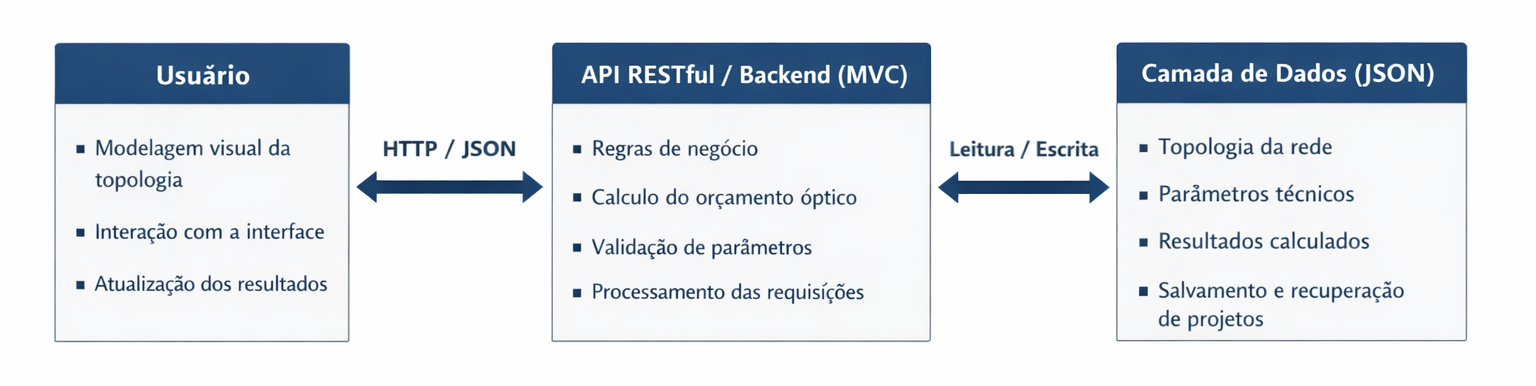
\includegraphics[width=\textwidth]{images/arquitetura_solucao.png}
		\par\footnotesize Fonte: Elaboração própria com auxilio de IA.
    }
\end{figure}

\section{Ferramentas e Tecnologias}

O desenvolvimento da aplicação será baseado em tecnologias voltadas a sistemas web interativos e modulares. No \textit{frontend}, serão utilizados \gls{html}, \gls{css} e \textit{JavaScript}, com apoio da biblioteca D3.js para a visualização interativa da topologia da rede \gls{pon}. No \textit{backend}, será empregada a linguagem Python, devido à sua simplicidade e adequação à implementação da lógica de negócio e dos cálculos de orçamento óptico. A \gls{api} \textit{RESTful} será desenvolvida com FastAPI, responsável pelo processamento das requisições, validação de dados e organização dos serviços conforme o padrão \gls{mvc}. A comunicação entre os componentes ocorrerá via \gls{http}, utilizando o formato \gls{json} para a troca de dados.

O ambiente de execução será padronizado com o uso de contêineres \textit{Docker}, garantindo a portabilidade da aplicação. Os projetos serão armazenados em arquivos no formato \gls{json}, permitindo a persistência, a recuperação e a reutilização das topologias desenvolvidas. Ferramentas de versionamento e apoio ao desenvolvimento serão empregadas ao longo da implementação, incluindo o uso da plataforma GitHub para gerenciamento e versionamento do código-fonte, bem como o ambiente de desenvolvimento Visual Studio Code (VS Code) para suporte à codificação, depuração e organização da aplicação.

\section{Metodologia de Desenvolvimento}

O desenvolvimento seguirá uma abordagem incremental e iterativa, permitindo a evolução progressiva do sistema a partir de versões parciais. Inicialmente, serão realizados o levantamento e a consolidação dos requisitos, considerando o objetivo geral do trabalho e os objetivos específicos relacionados à modelagem visual da topologia, ao cálculo automático do orçamento óptico, à definição da arquitetura de software e à persistência dos projetos. Em seguida, será conduzido o planejamento arquitetural, com definição das responsabilidades dos principais módulos e dos fluxos de comunicação necessários ao funcionamento da aplicação. O fluxo geral desse processo é sintetizado na Figura~\ref{fig:fluxo_metodologia_desenvolvimento}, que organiza as etapas adotadas neste trabalho \cite{pressman2014software,sommerville2016software}.

\begin{figure}[htb]
	\caption{Fluxo da metodologia de desenvolvimento}
	\label{fig:fluxo_metodologia_desenvolvimento}
    \centering
    \parbox{16cm}{
		\centering
		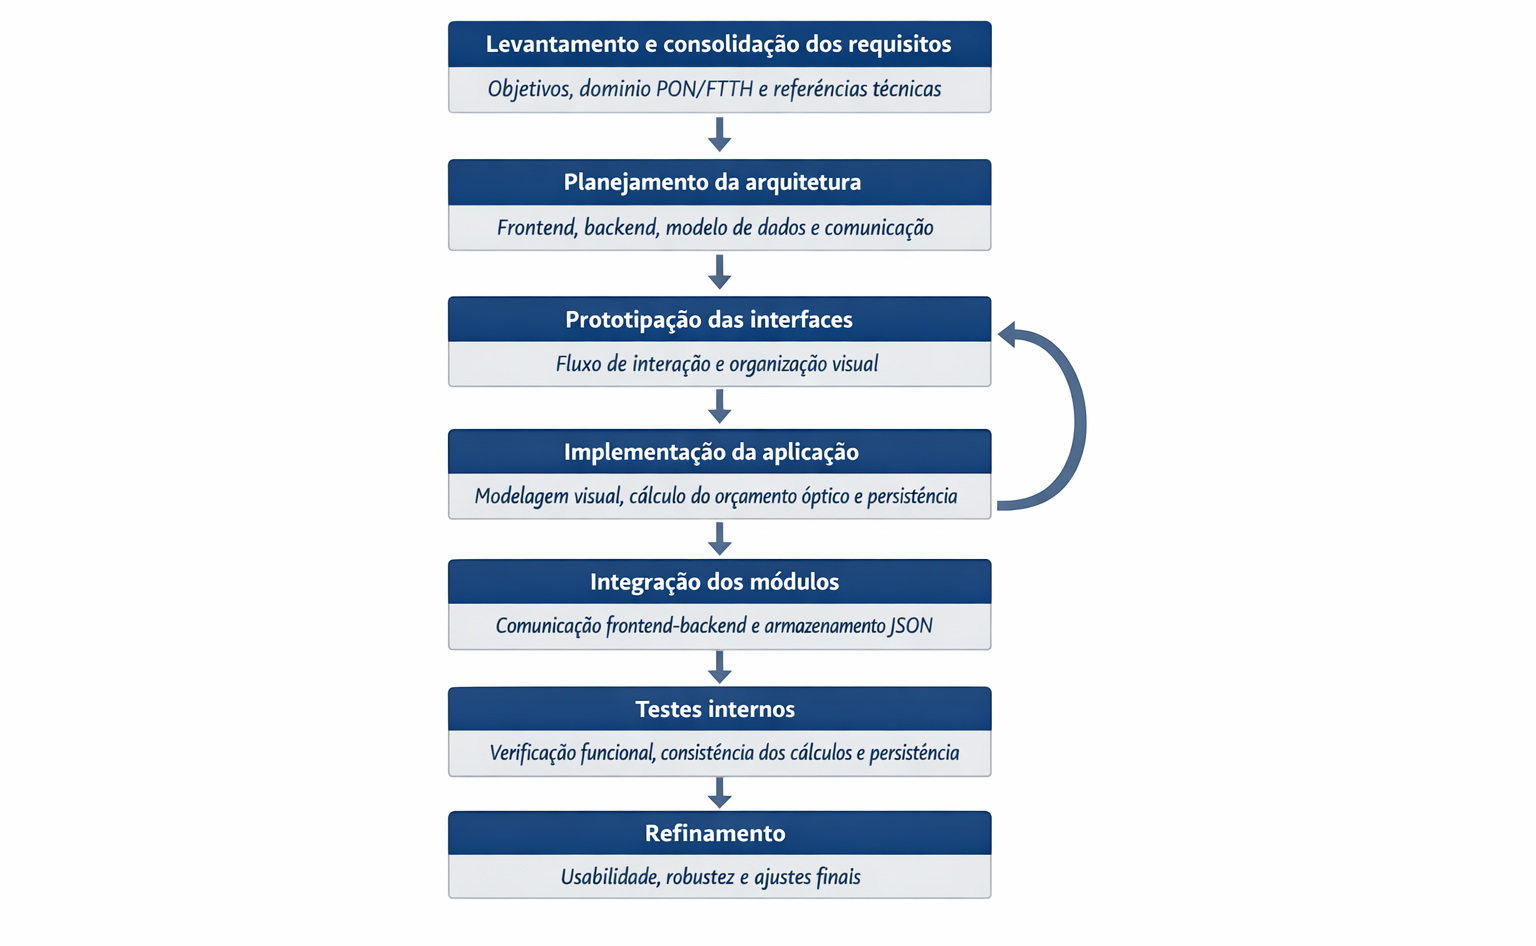
\includegraphics[width=\textwidth]{images/fluxo_metodologia_desenvolvimento.png}
		\par\footnotesize Fonte: Elaboração própria com auxilio de IA.
    }
\end{figure}

A Figura~\ref{fig:fluxo_metodologia_desenvolvimento}, demonstra as etapas de levantamento de requisitos, planejamento da arquitetura, prototipação das interfaces, implementação, integração dos módulos, testes internos e refinamento. A presença de realimentação entre as etapas finais evidencia o caráter iterativo do processo, no qual os resultados obtidos nos testes orientam ajustes sucessivos no sistema.

Na sequência, serão executadas as etapas de prototipação das interfaces, implementação da visualização para construção da topologia da rede, desenvolvimento das rotinas de cálculo do orçamento óptico e integração entre os módulos. A prototipação terá a função de antecipar a disposição dos elementos da interface e apoiar a definição do fluxo de interação do usuário. A implementação do \textit{backend} será realizada em Python, com estrutura modular para as rotinas de cálculo, as validações e os serviços da \gls{api}. Após a obtenção de uma versão funcional, serão realizados testes internos para verificar as funcionalidades implementadas, a consistência dos cálculos e a correta persistência e recuperação das estruturas modeladas.

Por fim, o sistema será submetido a uma etapa de refinamento, na qual eventuais ajustes identificados durante os testes serão incorporados com o objetivo de aprimorar a usabilidade, a clareza da visualização e a robustez do processamento. Como critério geral, busca-se assegurar que cada incremento preserve coerência arquitetural, funcionamento adequado e alinhamento com os objetivos definidos para o trabalho.

\subsection{Documentação dos requisitos e dos testes}

Os requisitos funcionais, não funcionais e as restrições do sistema são consolidados no Capítulo 5, juntamente com a descrição da arquitetura, da modelagem de dados e dos módulos implementados. O código-fonte e os arquivos de projeto permanecem versionados no repositório do GitHub, que funciona como registro das alterações realizadas durante o desenvolvimento. Para esta versão do trabalho, não foi adotado um sistema separado de histórias de usuários ou de casos de uso; as necessidades do sistema são descritas diretamente como requisitos e relacionadas às funcionalidades implementadas.

Os procedimentos de teste serão documentados na seção de resultados e análise do trabalho. Para cada caso serão apresentados a finalidade, a topologia utilizada, os parâmetros de entrada, o procedimento de execução, o resultado esperado, o resultado obtido e a diferença observada. Os testes automatizados correspondentes permanecem organizados nos arquivos do diretório \texttt{backend/tests}, enquanto os cálculos manuais de referência e os resultados consolidados serão apresentados em tabelas no texto. Dessa forma, o leitor poderá reproduzir a validação a partir da documentação acadêmica e conferir sua correspondência com os artefatos do repositório.

\section{Procedimentos de Validação e Análise}

A validação da solução será realizada por meio de cenários controlados e reproduzíveis, representativos do planejamento de redes ópticas \gls{pon}. Para cada cenário serão congelados a topologia, os parâmetros globais, os valores de potência e sensibilidade dos equipamentos e as perdas dos componentes. Os instrumentos de coleta serão constituídos pelos arquivos de projeto, pelos valores calculados pelo \textit{backend} e por uma tabela de referência elaborada independentemente do código.

O cálculo de referência será executado para cada caminho entre a \gls{olt} e uma \gls{onu}, aplicando a soma das perdas de fibra, conectores, fusões e \textit{splitters}. Serão comparados a perda total, a potência recebida, a margem disponível e o status do enlace. A diferença absoluta entre o resultado manual e o resultado do sistema deverá permanecer dentro da tolerância de arredondamento definida para o experimento, de 0,01~dB. Essa comparação verifica a implementação da fórmula sob os parâmetros adotados, não substituindo medições físicas em campo.

Os cenários deverão incluir um caminho simples, uma cascata de \textit{splitters}, um divisor desbalanceado, múltiplas \glspl{onu}, enlaces com caixas de emenda e fusões, um caso reprovado por margem insuficiente e uma topologia desbalanceada com ramificações de comprimentos e perdas distintas. Além da comparação numérica, serão observados o comportamento da interface durante a construção e a atualização da topologia e a capacidade de armazenamento e recuperação dos projetos em formato \gls{json}. O fluxo geral desse procedimento é sintetizado na Figura~\ref{fig:fluxo_validacao}, que apresenta as etapas de definição dos cenários, execução da aplicação, coleta dos registros e exame dos resultados.

Na Figura~\ref{fig:fluxo_validacao}, observam-se as etapas que compõem o processo de validação, desde a definição dos cenários de teste e a configuração dos parâmetros de entrada até a execução do sistema, a coleta dos registros gerados, a comparação com valores de referência e a análise dos resultados. Esse fluxo explicita a forma sistemática pela qual se pretende verificar a correção dos cálculos, a consistência funcional da aplicação e sua adequação aos objetivos definidos no trabalho.

\begin{figure}[htb]
	\caption{Fluxo de validação da solução}
	\label{fig:fluxo_validacao}
    \centering
    \parbox{16cm}{
		\centering
		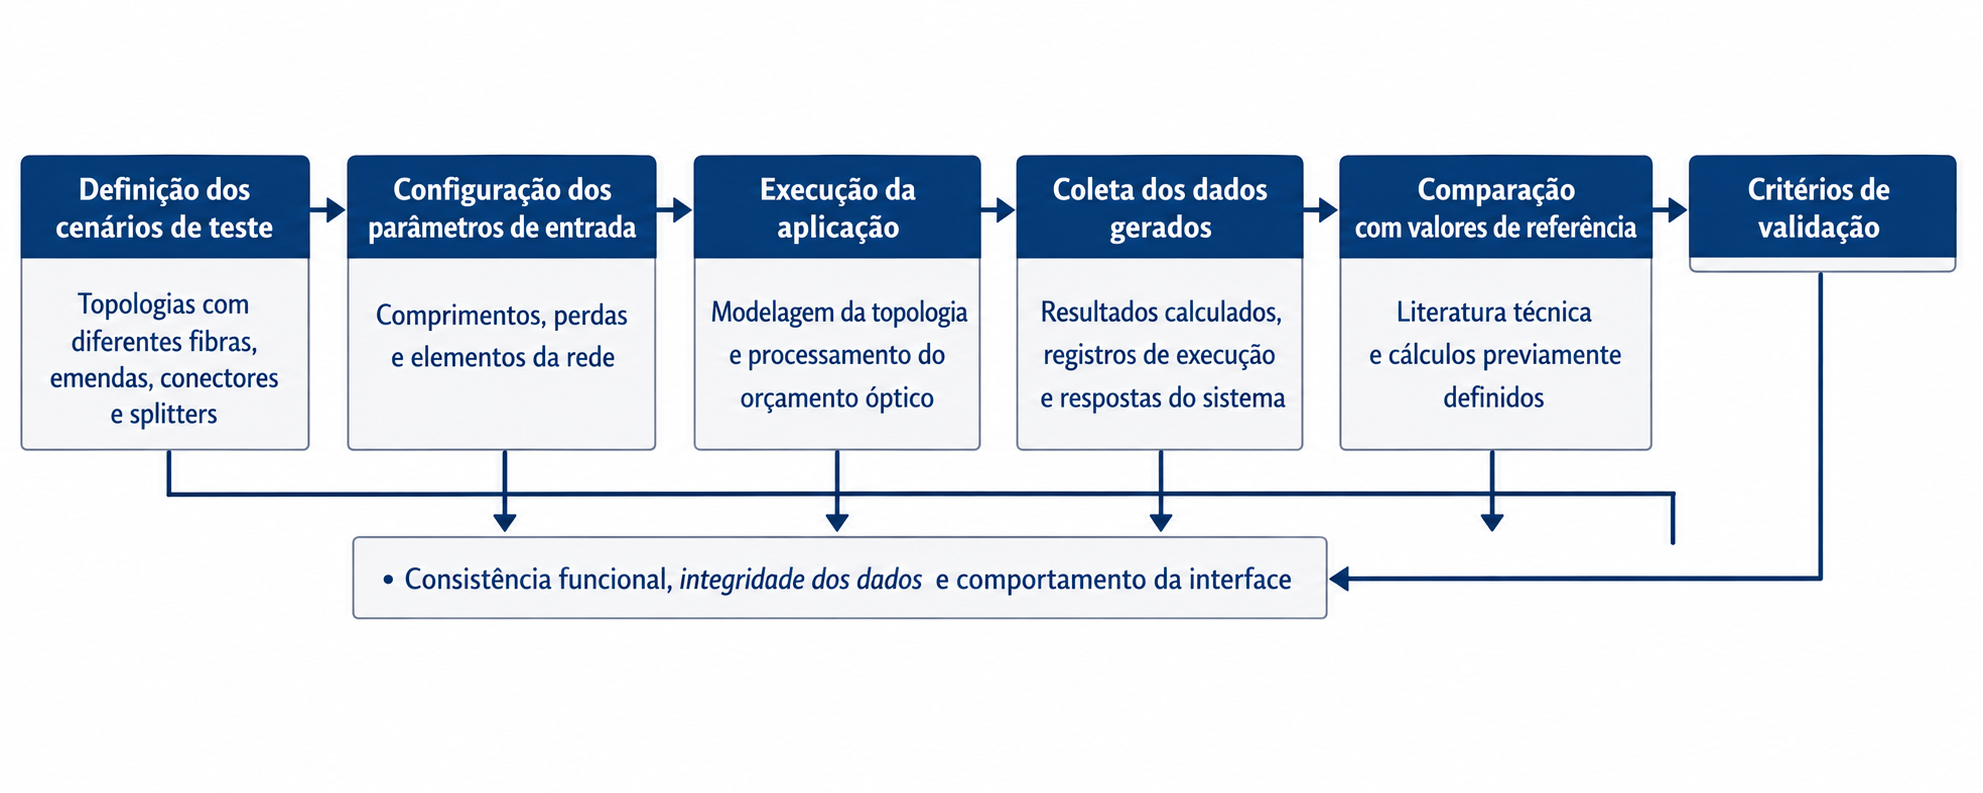
\includegraphics[width=\textwidth]{images/fluxo_validacao.png}
		\par\footnotesize Fonte: Elaboração própria com auxilio de IA.
    }
\end{figure}

A avaliação da solução considerará a correção das operações de modelagem, a consistência dos valores de orçamento óptico, o comportamento frente a diferentes estruturas de rede e a integridade dos dados. A ferramenta será considerada adequada quando os cenários apresentarem diferenças dentro da tolerância definida, os status calculados forem coerentes com as margens de referência e os projetos puderem ser persistidos e recuperados sem perda dos parâmetros relevantes.

\subsection{Avaliação de desempenho e escalabilidade visual}

O desempenho será analisado por meio de topologias com tamanhos crescentes, registrando a quantidade de nós, enlaces e caminhos \gls{olt}-\gls{onu}. Para cada tamanho serão coletadas várias execuções do endpoint de cálculo, considerando a média, o pior caso e os percentis de tempo. Quando possível, o tempo do \textit{backend} será separado do tempo de atualização visual no navegador. Essa avaliação permitirá identificar o comportamento do protótipo em redes maiores sem transformar uma medição pontual em garantia de desempenho para redes extremamente densas.

A interface utiliza D3.js com elementos \gls{svg}, escolha adequada para a manipulação customizada de nós, enlaces, zoom e arraste, mas que pode apresentar limitações à medida que a quantidade de elementos aumenta. Caso os testes indiquem degradação relevante, a renderização incremental, a agregação visual ou a adoção de Canvas/WebGL constituem alternativas para trabalhos futuros.

\subsection{Limitações e ameaças à validade}

O cálculo manual utiliza os mesmos pressupostos físicos e parâmetros de perda definidos no modelo, podendo reproduzir uma hipótese incorreta sem detectar limitações dos valores adotados. Além disso, os experimentos não substituem medições de campo, e a análise de desempenho depende do ambiente de execução. A utilização de arquivos \gls{json} simplifica a interoperabilidade e a persistência local, mas não avalia colaboração simultânea ou controle de conflitos em escala. Por fim, as classes ópticas B+, C+ e C++ são discutidas na fundamentação, enquanto a versão avaliada permite informar diretamente os parâmetros de potência e sensibilidade dos equipamentos, sem seleção automática por classe.

Do ponto de vista ético, o trabalho limita-se à análise técnica de um sistema computacional, sem envolvimento de dados pessoais ou participantes humanos, adotando princípios de integridade científica, rastreabilidade dos testes e transparência na apresentação dos resultados.


\chapter{Trabalhos Correlatos}

Este capítulo apresenta trabalhos acadêmicos e soluções tecnológicas relacionados à proposta deste estudo, com o objetivo de situar o tema no cenário atual e evidenciar lacunas ainda existentes na literatura e na prática. A análise considera abordagens que tratam do planejamento de redes \gls{ftth} baseadas em \gls{pon}, da representação da topologia de rede, da visualização de dados e da avaliação do desempenho óptico.

Os trabalhos selecionados foram organizados em dois grupos para facilitar a análise comparativa. Os primeiros itens correspondem a trabalhos acadêmicos que investigam o planejamento, a gestão, a visualização de redes ópticas e o uso de bibliotecas de grafos sob diferentes perspectivas. Os itens seguintes referem-se a ferramentas e softwares utilizados no mercado, o que permite contrastar abordagens teóricas e soluções práticas. Essa organização contribui para uma análise mais abrangente e para a identificação de convergências e limitações relevantes.

\section{Projeto e documentação de redes \gls{ftth} com uso de \gls{gis} e AutoCAD \cite{irjet2017ftth_gis_autocad}}

\citeonline{irjet2017ftth_gis_autocad} apresentam uma abordagem voltada ao projeto e à implementação de redes \gls{ftth} com apoio de ferramentas como \gls{gis} e AutoCAD. O estudo destaca procedimentos práticos relacionados à definição do traçado físico e à organização da infraestrutura, contribuindo especialmente para o entendimento da distribuição espacial dos componentes da rede. 

Como limitação, observa-se que a abordagem privilegia a dimensão física do projeto, com ênfase na representação geográfica dos ativos. A estrutura lógica da rede e a avaliação do desempenho do enlace não são exploradas de forma integrada, o que restringe o suporte ao planejamento técnico do sistema como um todo.


\section{Planejamento de redes \gls{ftth} com apoio de \gls{gis} \cite{rezgui2022qgis_ftth}}

\citeonline{rezgui2022qgis_ftth} investigam o uso do QGIS\footnote{O QGIS é um software de sistema de informação geográfica de código aberto, utilizado para visualizar, editar e analisar dados georreferenciados.} para o planejamento de redes \gls{ftth}, evidenciando o potencial das ferramentas de informação geográfica na organização espacial da infraestrutura e no mapeamento de rotas.

Embora a abordagem contribua para o entendimento territorial da rede, a modelagem permanece fortemente vinculada ao espaço geográfico, o que torna secundária a hierarquia lógica característica das arquiteturas \gls{pon}, especialmente o encadeamento entre \gls{olt}, \textit{splitters} e \glspl{onu}. Além disso, não há integração com mecanismos de avaliação do desempenho do enlace, o que limita a análise técnica do projeto.

\section{Gestão de redes \gls{ftth} com análise espacial e monitoramento por \gls{gis}  \cite{chakali2025gis_ftth}}

\citeonline{chakali2025gis_ftth} propõem uma solução baseada em \gls{gis} voltada à gestão de redes \gls{ftth}, integrando análise espacial, banco de dados geográfico e monitoramento de falhas. O trabalho amplia o escopo de aplicação de ferramentas computacionais ao abordar a operação e manutenção da infraestrutura. 

No entanto, o foco concentra-se na fase operacional da rede já implantada. Aspectos associados ao dimensionamento inicial, como definição estrutural da topologia e análise de viabilidade técnica, não constituem o núcleo da abordagem, evidenciando seu direcionamento para gestão e não para planejamento. Dessa forma, a ferramenta proposta neste estudo atua justamente na etapa anterior à gestão operacional, concentrando-se na validação técnica e no apoio ao planejamento que precedem a implantação da infraestrutura.

\section{Visualização interativa da topologia \gls{ftth} em ambiente web \cite{fatahillah2025visnetwork_ftth}}

\citeonline{fatahillah2025visnetwork_ftth} desenvolvem um sistema web para visualização interativa da topologia de redes \gls{ftth}, utilizando bibliotecas de grafos para representar relações entre dispositivos. O estudo reforça a importância da representação gráfica no apoio à compreensão de sistemas complexos. Em comparação com essa abordagem, a utilização da biblioteca D3.js na proposta deste trabalho oferece maior flexibilidade para manipulações customizadas dos dados e da interface, favorecendo a construção de visualizações mais aderentes às necessidades específicas do planejamento lógico de redes \gls{pon}. Esse contraste também evidencia a relevância de discutir, ainda que brevemente, o uso de bibliotecas JavaScript de grafos na literatura, especialmente quanto às possibilidades e limitações de integração com cálculos técnicos em tempo real.

Apesar do avanço na dimensão visual, a proposta não incorpora processos de avaliação técnica associados à transmissão óptica. Dessa forma, a ferramenta atua essencialmente na representação estrutural da rede, sem contemplar a análise do comportamento do enlace e o cálculo automatizado do orçamento de potência óptica.


\section{Visualização de topologias de redes com bibliotecas de grafos em JavaScript}

Diversos estudos na área de visualização de dados exploram o uso de bibliotecas JavaScript para a representação de grafos e redes complexas, com foco na interatividade e na manipulação dinâmica das estruturas apresentadas. Nesse contexto, destacam-se ferramentas como D3.js, Cytoscape.js e outras bibliotecas web utilizadas na construção de diagramas do tipo \textit{node-link}, amplamente aplicados na análise de redes sociais, biológicas e de informação. A biblioteca D3.js, em particular, tem sido reconhecida na literatura por sua capacidade de vincular dados diretamente aos elementos do documento e permitir a construção de visualizações altamente customizáveis, conforme apresentado por \citeonline{bostock2011d3}.

Apesar dos avanços proporcionados por essas bibliotecas, observa-se que grande parte das aplicações descritas na literatura concentra-se na representação visual das redes, com ênfase na disposição espacial dos nós, na interação do usuário e na análise estrutural dos grafos. Em geral, essas soluções são direcionadas à exploração visual e à navegação sobre estruturas relacionais, sem integração direta com modelos matemáticos ou cálculos técnicos específicos do domínio da aplicação. Assim, embora sejam eficazes para fins de visualização, apresentam limitações quando se trata da incorporação de cálculos especializados realizados de forma dinâmica e integrada à interface gráfica.

No contexto do planejamento de redes ópticas, especialmente em arquiteturas \gls{pon}, não foram identificados, na literatura analisada, trabalhos que integrem de forma direta a modelagem visual interativa da topologia com o cálculo automatizado do orçamento óptico em tempo real. Essa lacuna evidencia uma oportunidade de contribuição, uma vez que o uso do D3.js permite não apenas a construção de representações visuais interativas, mas também a manipulação direta dos dados associados aos elementos da rede. Dessa forma, a abordagem proposta neste trabalho diferencia-se das soluções puramente visuais ao integrar, em uma mesma aplicação, a visualização dinâmica da topologia e a análise técnica do enlace, proporcionando maior suporte ao processo de planejamento de redes ópticas.


\section{Plataforma georreferenciada para documentação de redes ópticas (GeoGrid Maps)}

O GeoGrid Maps é uma plataforma voltada à documentação e ao gerenciamento de redes de fibra óptica, oferecendo recursos de mapeamento georreferenciado, cadastro de infraestrutura e análise operacional da rede \cite{geogridmaps2026,geogrid_iclass_2026}. A ferramenta representa uma tendência de mercado que busca integrar inventário e gestão em um único ambiente. 

A Figura~\ref{fig:geogrid_mapa} ilustra a abordagem predominante desse tipo de solução, na qual a rede é representada com ênfase na localização geográfica dos elementos, evidenciando rotas, conexões físicas e distribuição espacial dos ativos. Nesse modelo, a visualização privilegia ``onde'' os componentes estão posicionados, facilitando atividades de documentação, operação e manutenção da infraestrutura. 

\begin{figure}[htb]
	\caption{Visualização georreferenciada da rede, destacando a localização dos elementos}
	\label{fig:geogrid_mapa}
    \centering
    \parbox{16cm}{
		\centering
		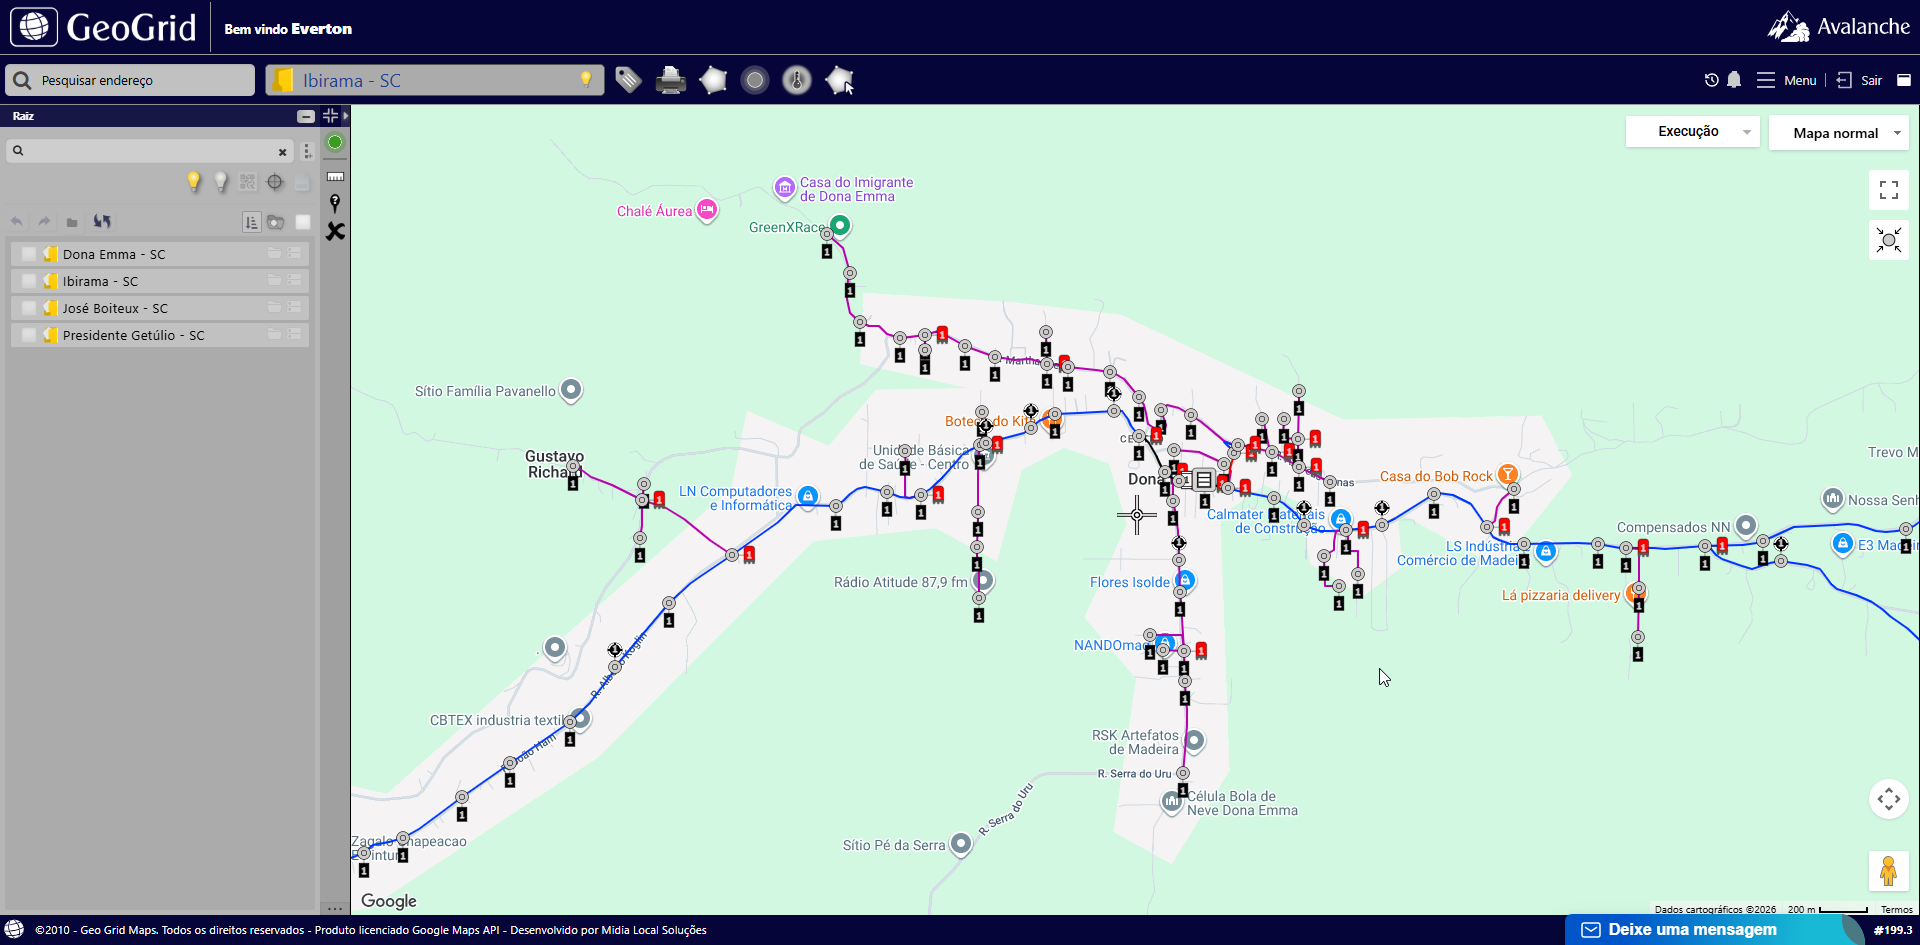
\includegraphics[width=\textwidth]{images/geogrid_mapa.png}
		\par\footnotesize Fonte: Adaptado da ferramenta GeoGrid Maps.
    }
\end{figure}

Adicionalmente, a Figura~\ref{fig:geogrid_ceo} exemplifica a representação detalhada de elementos internos da rede, como fusões em caixas de emenda, reforçando o caráter descritivo e cadastral dessas ferramentas, voltado à organização física dos componentes da rede óptica. 

\begin{figure}[htb]
	\caption{Detalhamento de fusões numa caixa de emenda}
	\label{fig:geogrid_ceo}
    \centering
    \parbox{16cm}{
		\centering
		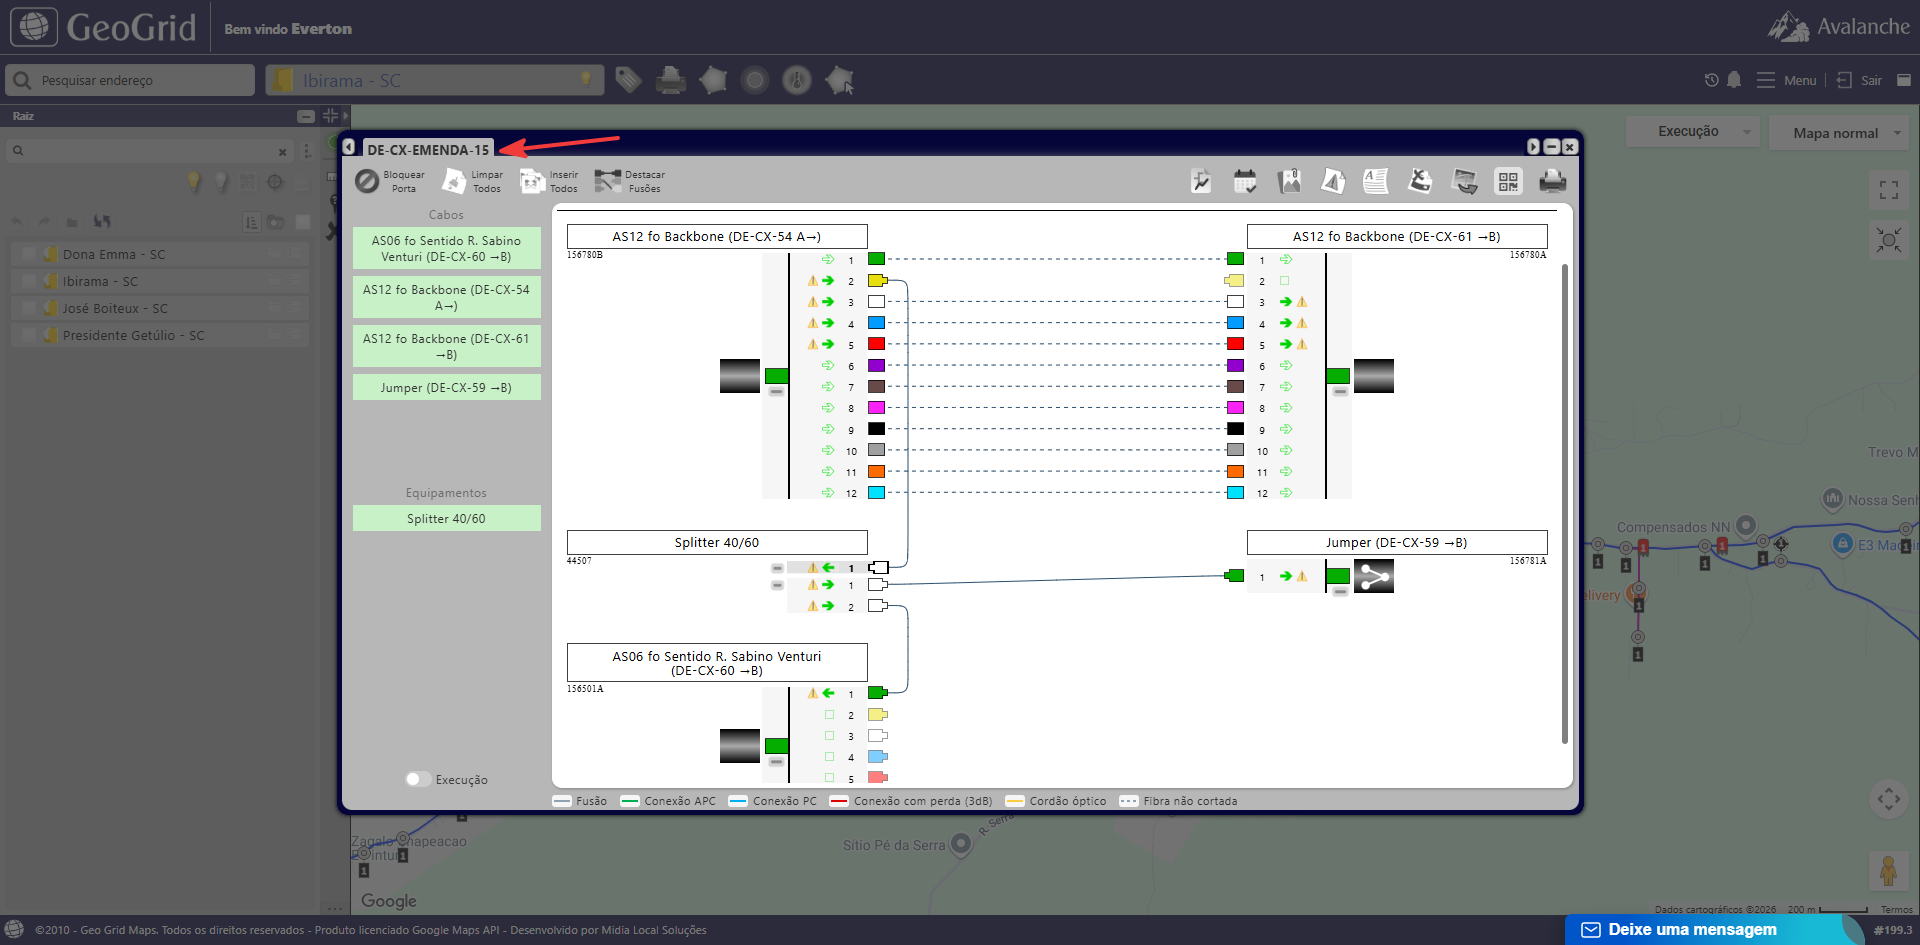
\includegraphics[width=\textwidth]{images/geogrid_ceo.png}
		\par\footnotesize Fonte: Adaptado da ferramenta GeoGrid Maps.
    }
\end{figure}

Apesar de sua relevância no contexto operacional, esse tipo de abordagem não atende plenamente ao problema tratado neste trabalho. Isso ocorre porque o foco permanece na representação geográfica e na documentação dos ativos, não contemplando de forma central a modelagem lógica da topologia da rede nem a análise integrada do orçamento óptico ao longo do enlace. Em geral, ferramentas dessa natureza funcionam sobretudo como repositórios estruturados de dados da rede: permitem cadastrar, organizar, consultar e visualizar informações sobre a infraestrutura implantada, mas tendem a pressupor que o usuário já possua o conhecimento técnico necessário para interpretar os parâmetros do projeto e realizar, por conta própria, os cálculos de validação do enlace. Dessa forma, embora essas soluções sejam adequadas para inventário, gestão e apoio à operação da rede implantada, elas não oferecem suporte direto à geração do conhecimento técnico associado ao planejamento lógico e à verificação automatizada da viabilidade óptica. Em contraste, a proposta desenvolvida neste trabalho busca justamente integrar a modelagem visual da rede à produção desse conhecimento técnico, por meio do cálculo automático do orçamento óptico, apoiando de forma mais direta o processo de planejamento e validação do enlace.

\section{Ferramenta de mapeamento e inventário de redes FTTx (OZmap)}

O OZmap é amplamente utilizado para mapeamento e documentação de redes FTTx, permitindo o cadastro e a visualização de elementos como cabos, caixas e clientes em ambiente georreferenciado \cite{ozmap2026,ozmap_help_2025}. A ferramenta destaca-se pela capacidade de organizar a infraestrutura e apoiar atividades de expansão e manutenção. 

A Figura~\ref{fig:ozmap_mapa} exemplifica a abordagem adotada por esse tipo de solução, na qual a rede é representada com base na sua distribuição geográfica. Observa-se que a visualização enfatiza a localização dos elementos no mapa, permitindo identificar rotas, posicionamento de caixas e distribuição da infraestrutura ao longo do território. Essa característica é particularmente útil para fins de inventário e operação da rede. 

\begin{figure}[htb]
	\caption{Visualização georreferenciada da rede no OZmap}
	\label{fig:ozmap_mapa}
    \centering
    \parbox{16cm}{
		\centering
		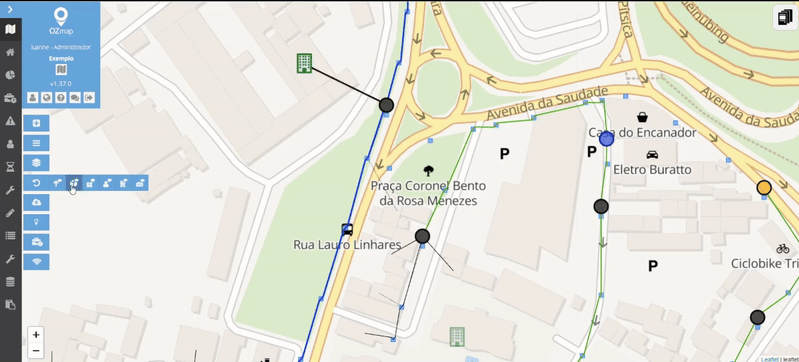
\includegraphics[width=\textwidth]{images/ozmap_mapa.png}
		\par\footnotesize Fonte: Adaptado da documentação do OZmap.
    }
\end{figure}

Além disso, esse modelo de visualização tende a dificultar a análise da estrutura lógica da rede, especialmente no contexto de arquiteturas \gls{pon}. Conforme ilustrado na Figura~\ref{fig:ozmap_diagrama}, a representação simultânea de múltiplos elementos, conexões e ramificações em um ambiente geográfico pode resultar em diagramas visualmente densos, com excesso de informações e baixa legibilidade da topologia de ponta a ponta. Essa sobreposição de elementos no espaço cartográfico pode gerar sobrecarga cognitiva, dificultando a percepção da continuidade lógica do sinal ao longo da rede e a compreensão clara do encadeamento entre seus componentes.

\begin{figure}[htb]
	\caption{Representação da rede com múltiplos elementos e alto nível de complexidade visual}
	\label{fig:ozmap_diagrama}
    \centering
    \parbox{16cm}{
		\centering
		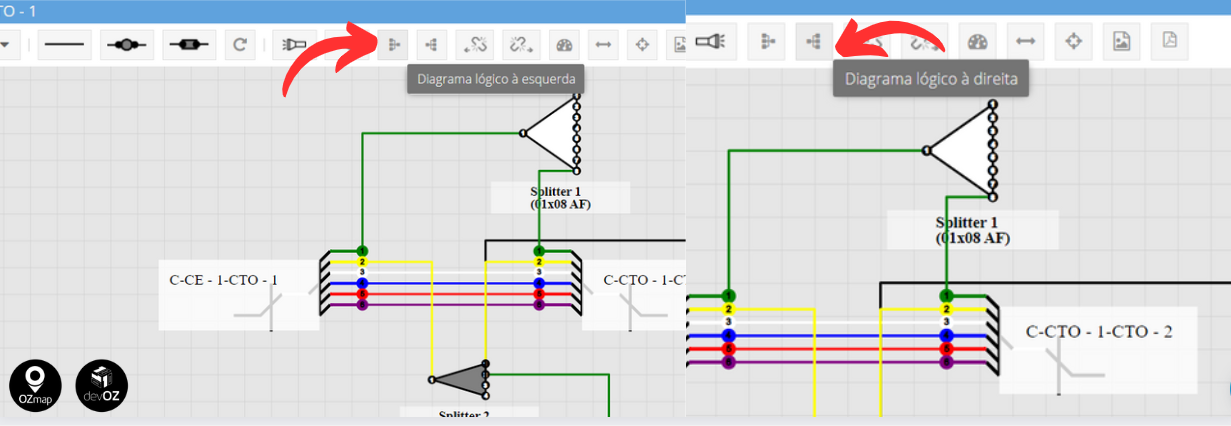
\includegraphics[width=\textwidth]{images/ozmap_diagrama.png}
		\par\footnotesize Fonte: Adaptado da documentação do OZmap.
    }
\end{figure}

Embora ferramentas como o OZmap sejam eficazes para documentação e gestão da rede implantada, elas não atendem plenamente ao problema abordado neste trabalho. Isso ocorre porque não oferecem uma representação orientada à compreensão lógica da topologia nem integram, de forma central, o cálculo do orçamento óptico ao processo de visualização. 

A limitação dessas soluções reside na dificuldade de apoiar o planejamento técnico do enlace, no qual é necessário compreender claramente a hierarquia da topologia ponto-multiponto e avaliar a viabilidade da transmissão óptica ao longo de toda a rede.


\section{Ferramenta de planejamento e documentação \gls{ftth} (FTTH Planner)}

O FTTH Planner apresenta-se como uma ferramenta voltada ao planejamento e à documentação de redes \gls{ftth}, oferecendo recursos para organização da infraestrutura e visualização de elementos em ambiente georreferenciado \cite{ftthplanner2026}. 

A Figura~\ref{fig:planner_mapa} ilustra a representação da rede com base na sua distribuição geográfica, evidenciando a localização dos elementos ao longo do território. Essa abordagem permite identificar rotas, posicionamento de caixas e organização da infraestrutura, sendo adequada para fins de planejamento físico e documentação da rede. 

\begin{figure}[htb]
	\caption{Visualização georreferenciada da rede no FTTH Planner}
	\label{fig:planner_mapa}
    \centering
    \parbox{16cm}{
		\centering
		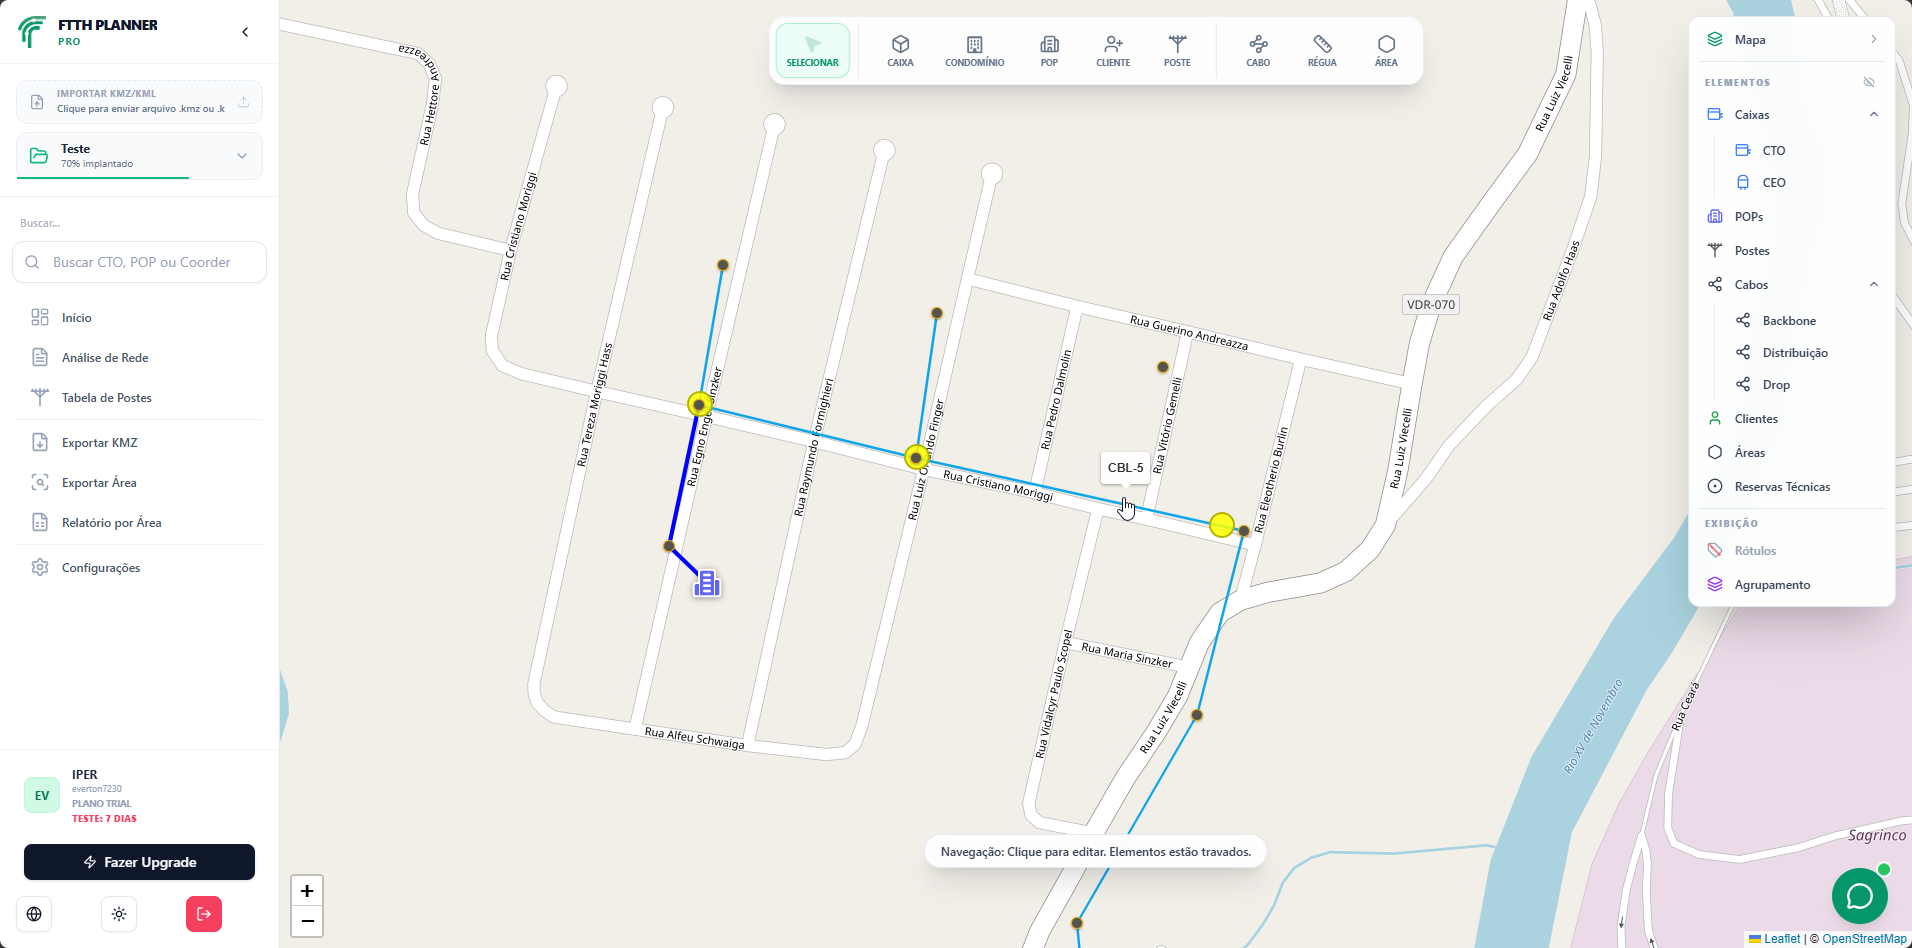
\includegraphics[width=\textwidth]{images/planner_mapa.png}
		\par\footnotesize Fonte: Adaptado do FTTH Planner.
    }
\end{figure}

Adicionalmente, a Figura~\ref{fig:planner_ceo} apresenta a visualização de fusões em caixas de emenda, destacando a forma como a ferramenta representa conexões internas da rede em nível local. Esse tipo de diagrama facilita a análise pontual de componentes específicos, especialmente para fins de organização e manutenção. 

\begin{figure}[htb]
	\caption{Representação de fusões em caixa de emenda no FTTH Planner}
	\label{fig:planner_ceo}
    \centering
    \parbox{16cm}{
		\centering
		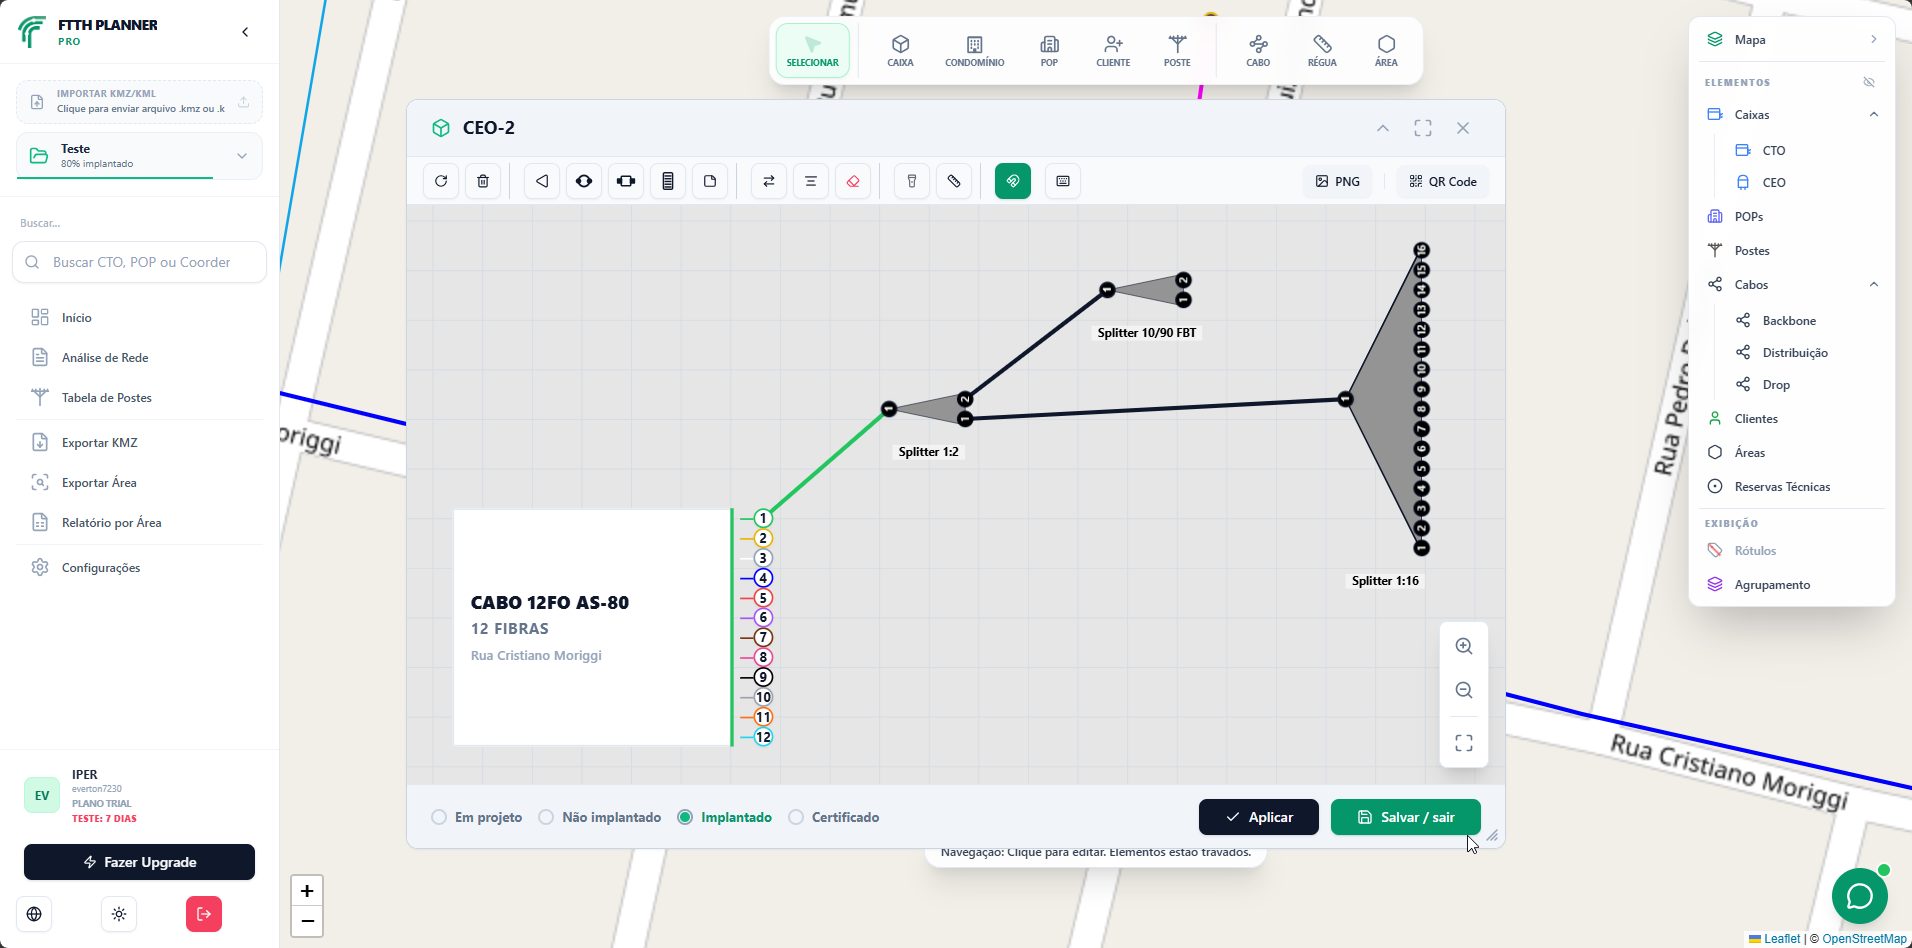
\includegraphics[width=\textwidth]{images/planner_ceo.png}
		\par\footnotesize Fonte: Adaptado do FTTH Planner.
    }
\end{figure}

A ferramenta não disponibiliza mecanismos para modelagem lógica completa da topologia da rede nem para o cálculo do orçamento óptico ao longo do enlace. A representação permanece concentrada na localização geográfica dos elementos e na visualização isolada de conexões em caixas, sem oferecer uma visão integrada do encadeamento da rede desde a origem até os pontos finais. 

Embora contribua para o registro e a organização da infraestrutura, o FTTH Planner não atende plenamente ao problema abordado neste trabalho, uma vez que não permite a análise conjunta da topologia lógica e do orçamento óptico. Essa limitação dificulta a validação técnica do projeto, a compreensão global do comportamento do enlace e a identificação de possíveis gargalos de potência ao longo da rede, aspectos centrais para o planejamento e a tomada de decisão técnica. Nesse sentido, a visão integrada proposta neste estudo amplia a utilidade prática da ferramenta ao apoiar não apenas a documentação da infraestrutura, mas também a análise da viabilidade óptica e a detecção antecipada de pontos críticos do enlace.


\section{Análise Comparativa}

De forma geral, os trabalhos acadêmicos revisados demonstram avanços importantes em aspectos específicos do planejamento de redes \gls{ftth}, como análise espacial, visualização de dados e gestão da infraestrutura. No entanto, esses aspectos são frequentemente tratados de maneira isolada, sem integração entre a modelagem da topologia lógica, a visualização interativa e o cálculo do orçamento óptico. 

As ferramentas de mercado, por sua vez, evidenciam a demanda prática por soluções integradas, especialmente no contexto de documentação e operação da rede. Ainda assim, a maioria delas privilegia o inventário e a gestão geográfica, com menor ênfase na análise técnica estruturada do enlace. 

A principal lacuna identificada não é a ausência de soluções, mas a falta de integração entre os elementos fundamentais discutidos na fundamentação teórica: representação visual da topologia, cálculo automatizado do orçamento óptico e apoio ao processo de planejamento. As Tabelas~\ref{tab:comparativo_trabalhos} e \ref{tab:comparativo_ferramentas} sintetizam essa leitura comparativa.

\begin{table}[htb]
    \centering
    \caption{Comparação entre trabalhos acadêmicos correlatos}
    \label{tab:comparativo_trabalhos}
    \small
    \begin{tabularx}{\textwidth}{|p{3.0cm}|X|c|c|X|}
        \hline
        \textbf{Trabalho} & \textbf{Foco principal} & \textbf{Vis. lógica} & \textbf{Cálculo óptico} & \textbf{Limitação principal} \\
        \hline
        Lokhande e Singh (2017) & Projeto físico de rede FTTH com GIS e AutoCAD & Não & Não & Ênfase no projeto físico da rede \\
        \hline
        Rezgui e Bourezg (2022) & Planejamento FTTH com apoio do QGIS & Parcial & Não & Foco espacial e documental \\
        \hline
        Chakali et al. (2025) & Gestão de rede com GIS e monitoramento de falhas & Parcial & Não & Ênfase em operação e manutenção \\
        \hline
        Fatahillah e Wulandari (2025) & Visualização web da topologia FTTH/OLT & Sim & Não & Não integra orçamento óptico \\
        \hline
        Proposta deste trabalho & Planejamento lógico de redes PON com apoio visual & Sim & Sim & Integra visualização, cálculo e persistência \\
        \hline
    \end{tabularx}
\end{table}

\begin{table}[htb]
    \centering
    \caption{Comparação entre ferramentas e softwares correlatos}
    \label{tab:comparativo_ferramentas}
    \small
    \begin{tabularx}{\textwidth}{|p{3.0cm}|X|c|c|X|}
        \hline
        \textbf{Ferramenta} & \textbf{Foco principal} & \textbf{Vis. lógica} & \textbf{Cálculo óptico} & \textbf{Limitação principal} \\
        \hline
        GeoGrid Maps & Documentação de rede e apoio operacional para provedores & Parcial & Parcial & Ênfase operacional e geográfica \\
        \hline
        OZmap & Mapeamento e documentação georreferenciada de redes FTTx & Parcial & Não central & Foco cartográfico e operacional \\
        \hline
        FTTH Planner & Registro de elementos georreferenciados e inventário & Parcial & Não & Ausência de cálculo integrado e foco geográfico \\
        \hline
        Proposta deste trabalho & Planejamento lógico de redes PON com apoio visual & Sim & Sim & Integra visualização, cálculo e persistência em contexto acadêmico\\
        \hline
    \end{tabularx}
\end{table}

\section{Posicionamento da Proposta}

Com base na análise dos correlatos, observa-se que a proposta deste trabalho se posiciona na interseção entre planejamento técnico de redes \gls{pon}, visualização de dados e desenvolvimento de aplicações web, com foco na integração desses elementos em um ambiente único. 

Diferentemente dos trabalhos acadêmicos analisados, que tendem a abordar isoladamente o planejamento geográfico, a visualização ou a gestão da rede, a proposta integra a modelagem visual interativa da topologia ponto-multiponto com o cálculo automatizado do orçamento óptico. Em relação às ferramentas de mercado, o foco desloca-se da documentação e operação para o apoio ao planejamento técnico, priorizando a compreensão lógica do enlace e a validação das decisões de projeto. 

A Figura~\ref{fig:diagrama_proposta} apresenta uma representação conceitual da abordagem proposta neste trabalho. O diagrama ilustra, de forma simplificada, a estrutura de uma rede óptica e os principais elementos que compõem o cálculo do orçamento óptico, até os terminais finais, bem como as perdas acumuladas ao longo do enlace. Essa representação, embora preliminar, auxilia na compreensão do objetivo da ferramenta a ser desenvolvida, destacando a integração entre a modelagem da topologia e a análise dos parâmetros técnicos da rede. 

\begin{figure}[htb]
	\caption{Representação conceitual da rede óptica e do cálculo do orçamento óptico}
	\label{fig:diagrama_proposta}
    \centering
    \parbox{16cm}{
		\centering
		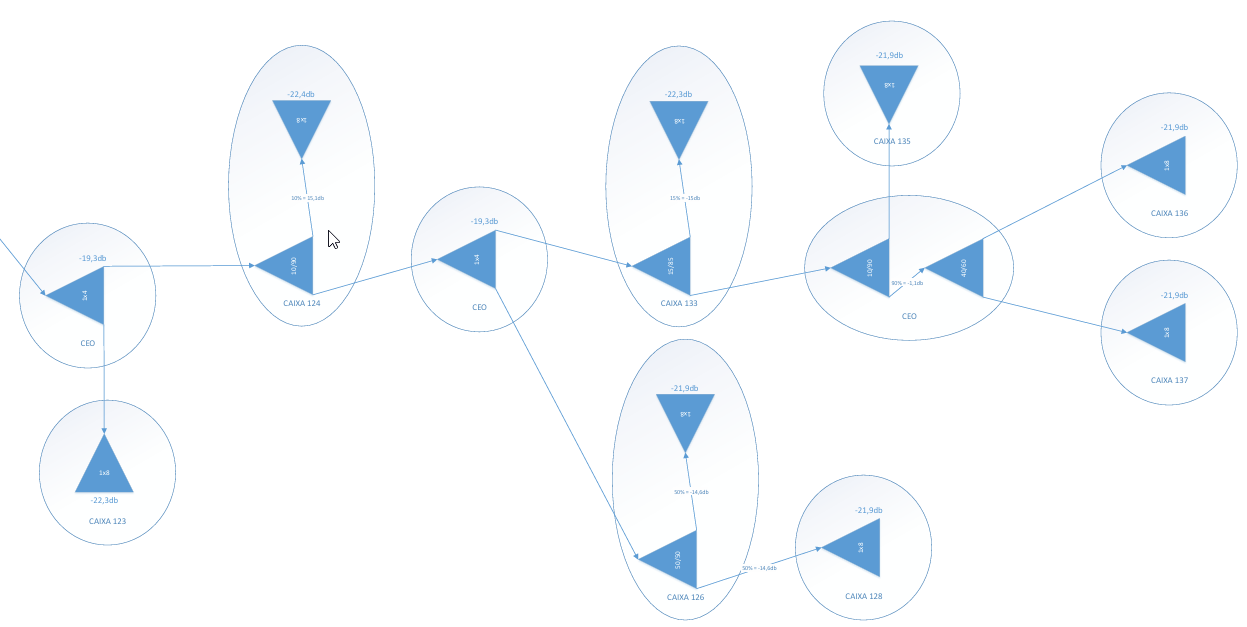
\includegraphics[width=\textwidth]{images/diagrama_proposta.png}
		\par\footnotesize Fonte: Elaboração própria.
    }
\end{figure}

Assim, a contribuição do trabalho não reside apenas na utilização de tecnologias conhecidas, mas na articulação entre seus componentes para atender a uma lacuna específica: a integração entre visualização, cálculo e modelagem da rede.

%\chapter{Considerações Finais}

As considerações apresentadas neste capítulo buscam sintetizar os principais aspectos do projeto desenvolvido, destacando sua relevância acadêmica e aplicada, bem como os resultados esperados com a implementação da solução proposta. Considerando que o trabalho ainda se encontra em fase de desenvolvimento, esta seção concentra-se na retomada dos objetivos definidos, nas contribuições pretendidas e nos encaminhamentos previstos para a continuidade da pesquisa e da construção da aplicação.

\section{Síntese da proposta e resultados esperados}

O presente projeto tem como propósito o desenvolvimento de uma aplicação web interativa voltada ao planejamento de redes ópticas \gls{ftth} baseadas em arquitetura \gls{pon}, integrando, em um mesmo ambiente, a modelagem visual da topologia da rede, o cálculo automatizado do orçamento óptico e o armazenamento estruturado das informações do projeto. A proposta foi concebida a partir da constatação de que o planejamento dessas redes, quando realizado com apoio de planilhas, diagramas isolados e procedimentos manuais, tende a demandar maior esforço operacional, além de apresentar limitações quanto à clareza da representação da topologia e à validação técnica dos enlaces.

Nesse contexto, espera-se que a solução proposta contribua para tornar o processo de planejamento mais claro, organizado e tecnicamente confiável, ao permitir que o projetista visualize a estrutura lógica da rede e acompanhe, de forma integrada, os impactos das escolhas topológicas sobre o orçamento óptico. Como resultados esperados, prevê-se a obtenção de uma aplicação funcional capaz de representar os principais elementos de uma rede \gls{pon}, processar automaticamente os cálculos associados às perdas ópticas e possibilitar o armazenamento e a recuperação dos projetos desenvolvidos. Além disso, espera-se que a aplicação constitua um instrumento de apoio tanto à elaboração quanto à análise de projetos, favorecendo a compreensão do encadeamento dos componentes da rede e auxiliando a tomada de decisão em cenários de planejamento.

Do ponto de vista acadêmico, o projeto busca contribuir para a discussão sobre o uso integrado de visualização de dados e processamento técnico no contexto de redes ópticas, articulando conceitos de telecomunicações, desenvolvimento web e arquitetura de software em uma solução aplicada. Do ponto de vista prático, pretende-se oferecer uma ferramenta que possa apoiar a validação prévia de projetos de redes \gls{ftth}, reduzindo a dependência de processos fragmentados e favorecendo maior consistência na análise dos enlaces. Como etapa seguinte, o desenvolvimento da aplicação será conduzido conforme o cronograma proposto, abrangendo a implementação dos módulos previstos, sua integração, a realização de testes em cenários controlados e a análise dos resultados obtidos. Assim, entende-se que este projeto estabelece uma base coerente e tecnicamente fundamentada para a continuidade do trabalho no TCC final.

\section{CRONOGRAMA}

Este capítulo apresenta o cronograma previsto para a execução das etapas do projeto, contemplando as atividades de fundamentação teórica, modelagem, desenvolvimento, integração, validação e redação final do trabalho. A organização temporal das etapas busca assegurar a condução progressiva e coerente da pesquisa e da implementação da aplicação proposta.

\begin{table}[h]
\caption{Cronograma de execução do TCC}
\label{tab:cronograma}
\centering
\resizebox{\textwidth}{!}{
\begin{tabular}{|
    >{\RaggedRight\hspace{0pt}}m{8cm}|
    >{\Centering\hspace{0pt}}m{1cm}|
    >{\Centering\hspace{0pt}}m{1cm}|
    >{\Centering\hspace{0pt}}m{1cm}|
    >{\Centering\hspace{0pt}}m{1cm}|
    >{\Centering\hspace{0pt}}m{1cm}|
    >{\Centering\hspace{0pt}}m{1cm}|
    >{\Centering\hspace{0pt}}m{1cm}|
}
\hline
\textbf{Etapa} & \textbf{Jul} & \textbf{Ago} & \textbf{Set} & \textbf{Out} & \textbf{Nov} & \textbf{Dez} \\
\hline Revisão bibliográfica, levantamento de requisitos e definição da arquitetura da solução & X & X & & & & \\
\hline Modelagem do sistema, prototipação da interface e definição da estrutura de dados & & X & X & & & \\
\hline Desenvolvimento do \textit{backend} e implementação da lógica de cálculo do orçamento óptico & & X & X & & & \\
\hline Desenvolvimento do \textit{frontend} e implementação da visualização interativa & & & X & X & & \\
\hline Integração dos módulos, persistência dos dados e testes funcionais & & & & X & X & \\
\hline Validação da aplicação, refinamento e ajustes finais & & & & & X & X \\
\hline Redação da monografia e preparação da apresentação final & X & X & X & X & X & X \\
\hline
\end{tabular}
}

\vspace{3pt}
{\raggedright \noindent Fonte: Elaboração Própria.}
\end{table}
\renewcommand{\arraystretch}{1}

\begin{description}[style=nextline, leftmargin=0cm, itemsep=0.5em]
    \item[Revisão bibliográfica, levantamento de requisitos e definição da arquitetura.] Prevista para julho e agosto, essa etapa concentra o aprofundamento da fundamentação teórica, a consolidação dos requisitos do sistema e a definição da arquitetura geral da aplicação, estabelecendo as bases conceituais e técnicas do projeto.
    \item[Modelagem do sistema, prototipação da interface e definição da estrutura de dados.] Desenvolvida entre agosto e setembro, essa etapa compreende a organização lógica dos módulos da aplicação, a elaboração dos protótipos de interface e a definição da estrutura dos dados que representarão a topologia da rede e os parâmetros técnicos associados.
    \item[Desenvolvimento do \textit{backend} e implementação da lógica de cálculo do orçamento óptico.] Previsto para agosto e setembro, contempla a implementação da \gls{api}, das regras de negócio, das validações e das rotinas responsáveis pelo processamento dos cálculos ópticos da aplicação.
    \item[Desenvolvimento do \textit{frontend} e implementação da visualização interativa.] Distribuída entre setembro e outubro, essa etapa envolve a construção da interface web da aplicação e da visualização interativa da topologia da rede, permitindo a modelagem gráfica dos elementos e a interação do usuário com o sistema.
    \item[Integração dos módulos, persistência dos dados e testes funcionais.] Prevista para outubro e novembro, essa etapa corresponde à integração entre \textit{frontend} e \textit{backend}, à implementação do armazenamento das informações da rede e à realização de testes funcionais para verificação do comportamento da aplicação.
    \item[Validação da aplicação, refinamento e ajustes finais.] Desenvolvida entre novembro e dezembro, essa etapa compreende a execução dos cenários de teste, a comparação dos resultados obtidos com valores de referência e a incorporação de ajustes necessários ao aprimoramento da solução.
    \item[Redação da monografia e preparação da apresentação final.] Realizada de forma contínua ao longo de todo o período, essa etapa envolve a consolidação da escrita acadêmica do trabalho, a revisão do texto e a preparação do material a ser apresentado à banca examinadora.
\end{description}
\chapter{Desenvolvimento}

Neste capítulo, apresento detalhadamente todas as etapas envolvidas no desenvolvimento da plataforma web para projeto, visualização gráfica e cálculo automatizado do orçamento óptico em redes \gls{pon}. A abordagem contempla desde o planejamento inicial até a consolidação da solução computacional. Inicialmente, estabeleço a especificação dos requisitos funcionais e não funcionais, bem como as restrições técnicas e operacionais que orientaram o projeto. Em seguida, descrevo o processo de prototipação da interface gráfica (\textit{wireframes}) e a definição da arquitetura de software adotada. Na sequência, detalho a modelagem de dados serializada em formato \gls{json}, os diagramas arquiteturais e os fluxos e algoritmos de cálculo de atenuação óptica codificados no \textit{backend}. Por fim, apresento a implementação prática da solução, detalhando a estrutura modular do código-fonte em FastAPI, a integração com a biblioteca gráfica D3.js no \textit{frontend} e o ambiente de conteinerização para implantação do sistema.

\section{Análise e Especificação de Requisitos}

Na etapa de análise e especificação de requisitos busquei mapear as necessidades operacionais de projetistas e engenheiros de redes \gls{ftth}/\gls{pon}, garantindo que o sistema ofereça precisão matemática nos cálculos de atenuação e facilidade de manipulação visual da topologia. A seguir, são detalhados os requisitos funcionais, os requisitos não funcionais e as restrições do sistema.

\subsection{Requisitos Funcionais}

Os Requisitos Funcionais descrevem as ações, cálculos e comportamentos que o sistema deve executar para atender às necessidades do usuário:

\begin{itemize}
    \item \textbf{Criação e Edição Interativa da Topologia:} O sistema deve permitir ao usuário construir e modificar visualmente a árvore da rede, inserindo, movendo e removendo elementos típicos de rede \gls{pon}, tais como \gls{olt}, caixas de emenda/fusão, \textit{splitters} (balanceados e desbalanceados), \gls{cto} e \gls{onu}.
    
    \item \textbf{Cálculo Automatizado do Orçamento Óptico:} O sistema deve calcular automaticamente a perda acumulada de potência ao longo de cada enlace, considerando a atenuação distribuída da fibra por quilômetro.
    
    \item \textbf{Contabilização de Atenuações Concentradas:} O sistema deve computar as perdas pontuais de inserção introduzidas por conectores ópticos, emendas/fusões de fibra e elementos passivos de divisão (\textit{splitters} balanceados e desbalanceados).
    
    \item \textbf{Validação por Classe de Transceptor:} O sistema deve parametrizar e validar os níveis de potência de transmissão ($T_x$) e os limites de sensibilidade do receptor ($R_x$) de acordo com as classes normatizadas.
    
    \item \textbf{Indicação do Status do Link:} O sistema deve sinalizar visualmente em tempo real se a potência óptica que atinge cada nó de terminação \gls{onu} está dentro dos limites operacionais adequados, exibindo alertas em caso de sinal degradado ou fora da margem de sensibilidade.
    
    \item \textbf{Persistência de Projetos em \gls{json}:} O sistema deve permitir salvar, carregar, atualizar e exportar a estrutura completa da topologia da rede e seus parâmetros de configuração em arquivos no formato \gls{json}.
    
    \item \textbf{Gerenciamento de Projetos e Pastas:} O sistema deve fornecer uma interface para organização de múltiplos arquivos de projeto dentro de diretórios no ambiente do servidor.
\end{itemize}

\subsection{Requisitos Não Funcionais}

Os Requisitos Não Funcionais definem os critérios de qualidade, desempenho, usabilidade e infraestrutura exigidos pela aplicação:

\begin{itemize}
    \item \textbf{Arquitetura em Camadas e Desacoplamento:} O \textit{backend} deve ser implementado em Python utilizando o \textit{framework} FastAPI, seguindo o padrão de projeto \gls{mvc} para separação clara entre rotas, regras de negócio e persistência.
    
    \item \textbf{Renderização Gráfica de Alto Desempenho:} A interface gráfica (\textit{frontend}) deve utilizar a biblioteca manipuladora de grafos D3.js no navegador, garantindo renderização fluida e reativa da estrutura da rede em tempo real.
    
    \item \textbf{Portabilidade e Conteinerização:} A aplicação deve fornecer suporte completo a contêineres Docker e orquestração via Docker Compose, permitindo execução simples e padronizada em ambientes de desenvolvimento e produção independente do sistema operacional hospedeiro.
    
    \item \textbf{Baixo Tempo de Resposta:} As chamadas à \gls{api} REST para recalculo do orçamento óptico devem responder em tempo inferior a 200 milissegundos.
    
\end{itemize}

\subsection{Restrições do Sistema}

O escopo do desenvolvimento esteve sujeito às seguintes restrições técnicas e operacionais:

\begin{itemize}
    \item O sistema opera focado no cálculo de potência unidirecional do canal de \textit{downstream}. Não calcula a potência no sentido \textit{upstream}
    
    \item A persistência local é realizada diretamente no sistema de arquivos em formato \gls{json}, abrindo mão de um banco de dados para simplificar a implantação.
    
    \item O motor de visualização limita-se à representação lógica da topologia em formato de grafo em árvore ponto-multi-ponto, sem integração georreferenciada.
\end{itemize}

\subsection{Prototipação da Interface (Wireframes)}

Antes do início da codificação da interface gráfica final, elaborei protótipos de interface (\textit{wireframes}). O objetivo dessa etapa foi organizar a arquitetura de informação e validar a usabilidade do operador antes da integração com a biblioteca gráfica D3.js e o motor de cálculo.

A interface foi concebida em três áreas funcionais integradas:
\begin{itemize}
    \item \textbf{Barra de Ferramentas Lateral (\textit{Toolbar}):} Disposta à esquerda, agrupando os atalhos para inserção dos elementos de rede (\gls{olt}, \textit{Splitters} balanceados e desbalanceados, \gls{onu} e Caixas de Anotação/Texto).
    
    \item \textbf{Área Central de Modelagem (\textit{Canvas}):} Espaço interativo principal onde a topologia gráfica é desenhada e manipulada via arrasto, renderizando os enlaces de fibra e caixas de atendimento.
    
    \item \textbf{Painel de Propriedades e Orçamento Óptico:} Coluna lateral à direita dedicada à edição dos parâmetros do nó selecionado e exibição em tempo real do nível de sinal calculado.
\end{itemize}

A Figura~\ref{fig:wireframe_interface} ilustra a concepção estrutural da interface do sistema.

\begin{figure}[htb]
    \caption{Esquema de \textit{wireframe} para a interface de modelagem gráfica}
    \centering
    \parbox{16cm}{
        \centering
        \label{fig:wireframe_interface}
        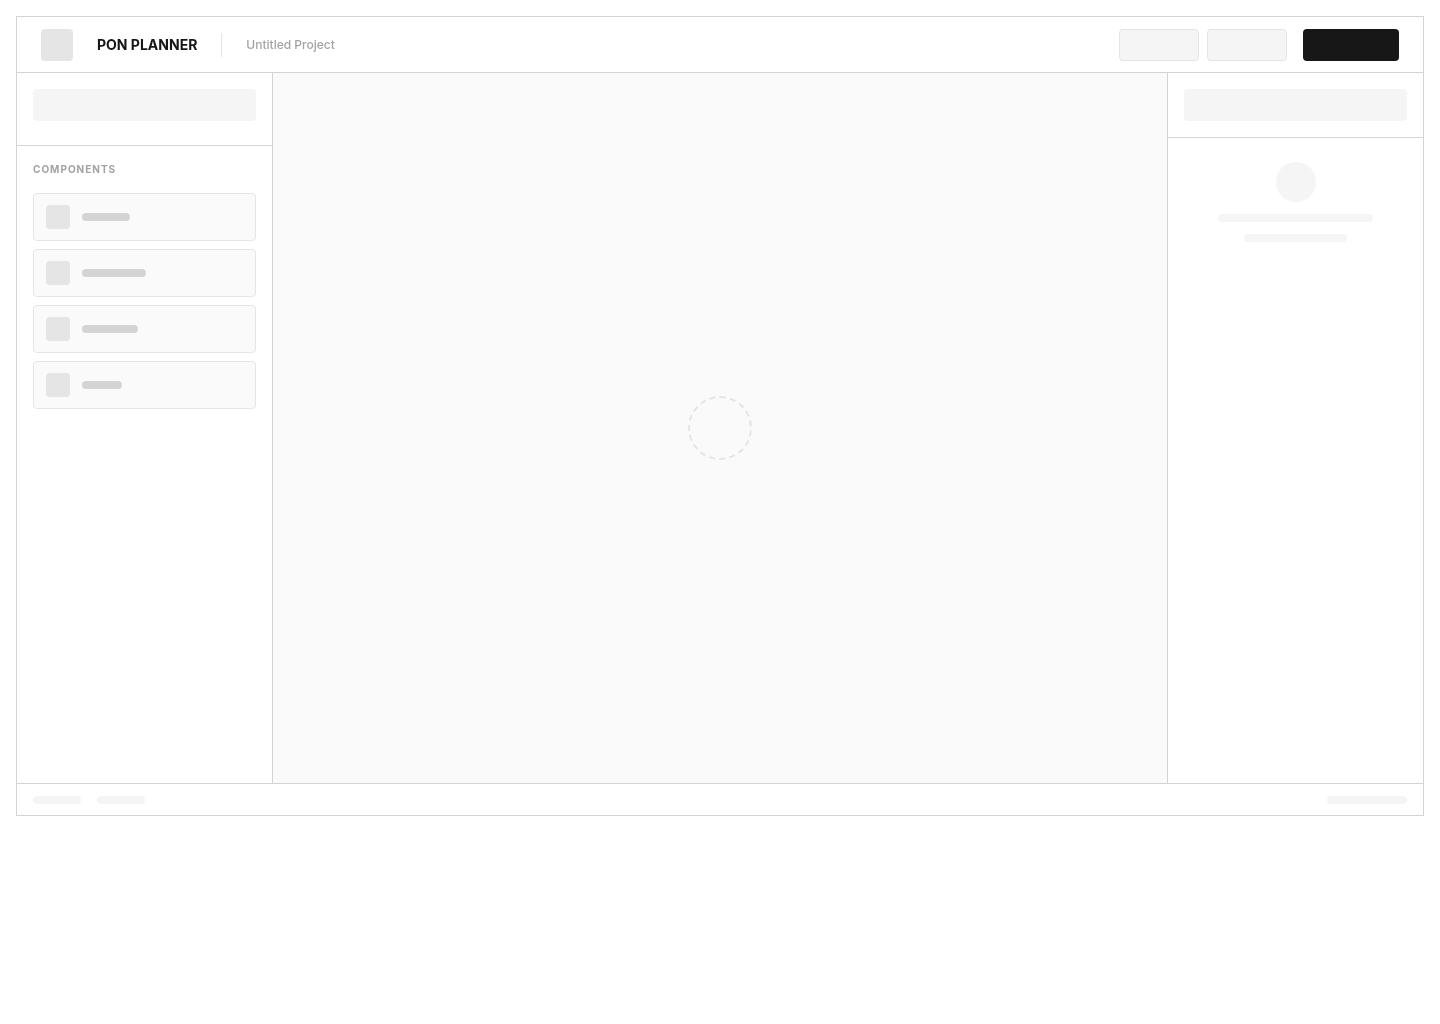
\includegraphics[width=\textwidth]{images/wireframe_interface.png}
        \par\footnotesize Fonte: Elaboração própria com auxílio de IA.
    }
\end{figure}

\section{Arquitetura do Sistema}

A arquitetura de software da plataforma foi desenvolvida com base no desacoplamento entre a camada de apresentação (\textit{frontend}) e a camada de serviços e regras de negócio (\textit{backend}). Essa abordagem garante modularidade, facilita a manutenção do código e permite que o cálculo do orçamento óptico seja consumido como um serviço independente por meio de uma \gls{api} RESTful. A seguir, detalho a visão geral da arquitetura, a organização de seus componentes internos e o modelo de implantação conteinerizado.

\subsection{Visão Geral da Arquitetura}

O sistema adota o padrão cliente-servidor para aplicações web de página única \gls{spa}. O \textit{frontend} é executado diretamente no navegador do usuário, sendo responsável por renderizar a interface gráfica e capturar interações da topologia. A comunicação com o \textit{backend} ocorre de forma assíncrona por meio de requisições \gls{http} enviando e recebendo dados estruturados em formato \gls{json}.

Na Figura~\ref{fig:arquitetura_geral}, apresento a visão geral da arquitetura do sistema e o fluxo de interação entre o usuário, o cliente web e o servidor de aplicação.

\begin{figure}[htb]
    \caption{Visão geral da arquitetura do sistema}
    \centering
    \parbox{16cm}{
        \centering
        \label{fig:arquitetura_geral}
        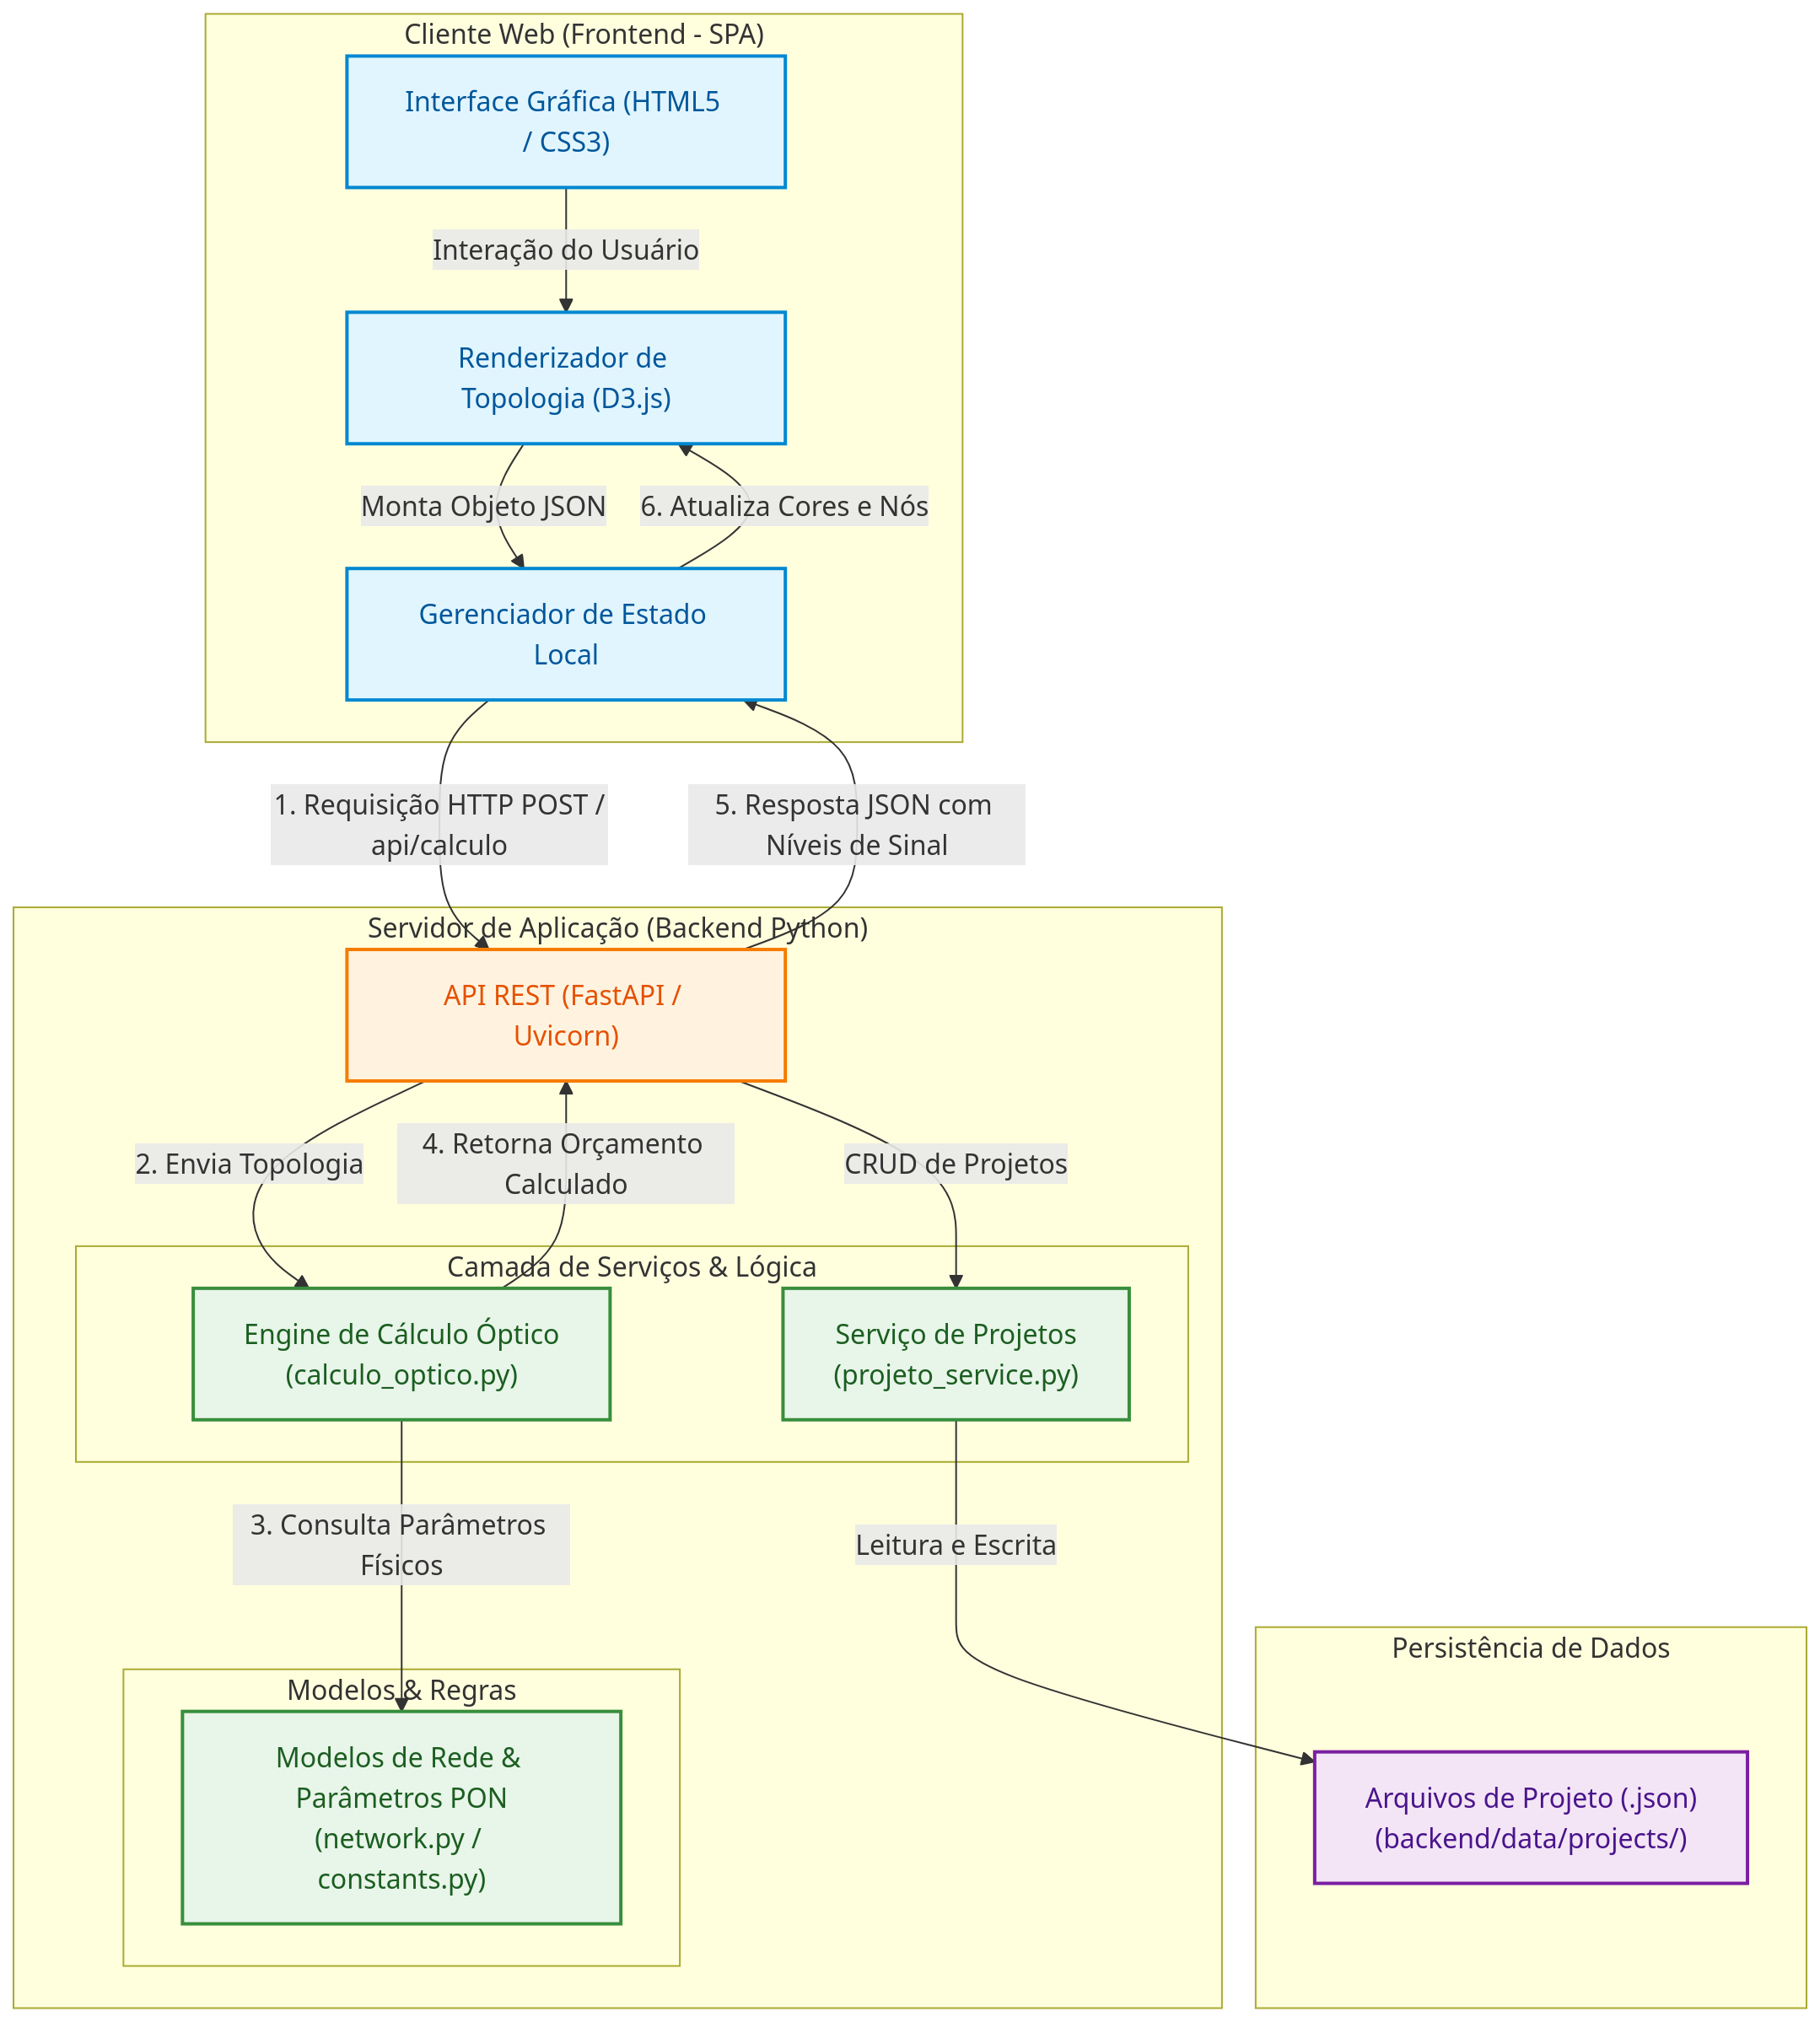
\includegraphics[width=\textwidth]{images/arquitetura_geral.png}
        \par\footnotesize Fonte: Elaboração própria com auxílio de IA.
    }
\end{figure}

Ao realizar qualquer alteração na topologia (como adicionar um nó ou alterar o comprimento de um trecho de fibra), o \textit{frontend} monta o objeto da rede em \gls{json} e o dispara para o \textit{endpoint} de cálculo do \textit{backend}. O servidor processa a topologia, efetua a soma das atenuações e retorna os níveis de sinal calculados para cada nó, permitindo a atualização imediata da interface visual.

\subsection{Diagrama de Componentes}

O \textit{backend} foi estruturado sob o padrão \gls{mvc}, utilizando o \textit{framework} FastAPI. A organização dos componentes é subdividida em três camadas principais:

\begin{itemize}
    \item \textbf{Controladores (\textit{Controllers}):} Módulos responsáveis por expor as rotas da \gls{api} REST e tratar as requisições \gls{http}. O controlador \texttt{calculo.py} recebe as estruturas de rede para validação e recalculo; o controlador \texttt{projetos.py} lida com operações de criação, leitura, atualização e exclusão de arquivos de topologia; e o controlador \texttt{pastas.py} gerencia a organização dos arquivos no servidor.
    
    \item \textbf{Serviços (\textit{Services}):} Concentram a lógica de negócio do sistema. O serviço \texttt{calculo\_optico.py} contém os algoritmos matemáticos que percorrem a árvore da rede e somam as perdas distribuídas e concentradas. O serviço \texttt{projeto\_service.py} gerencia o manuseio e a serialização de dados no sistema de arquivos.
    
    \item \textbf{Modelos e Constantes (\textit{Models}):} O arquivo \texttt{network.py} estabelece as estruturas de dados para representação de nós, conexões e redes. O arquivo \texttt{constants.py} armazena os parâmetros físicos normatizados, tais como coeficientes de atenuação de conectores, emendas, \textit{splitters}.
\end{itemize}

A Figura~\ref{fig:diagrama_componentes} ilustra o Diagrama de Componentes do sistema, detalhando a divisão modular interna e as dependências entre controladores, serviços e modelos.

\begin{figure}[htb]
    \caption{Diagrama de componentes do \textit{backend}}
    \centering
    \parbox{16cm}{
        \centering
        \label{fig:diagrama_componentes}
        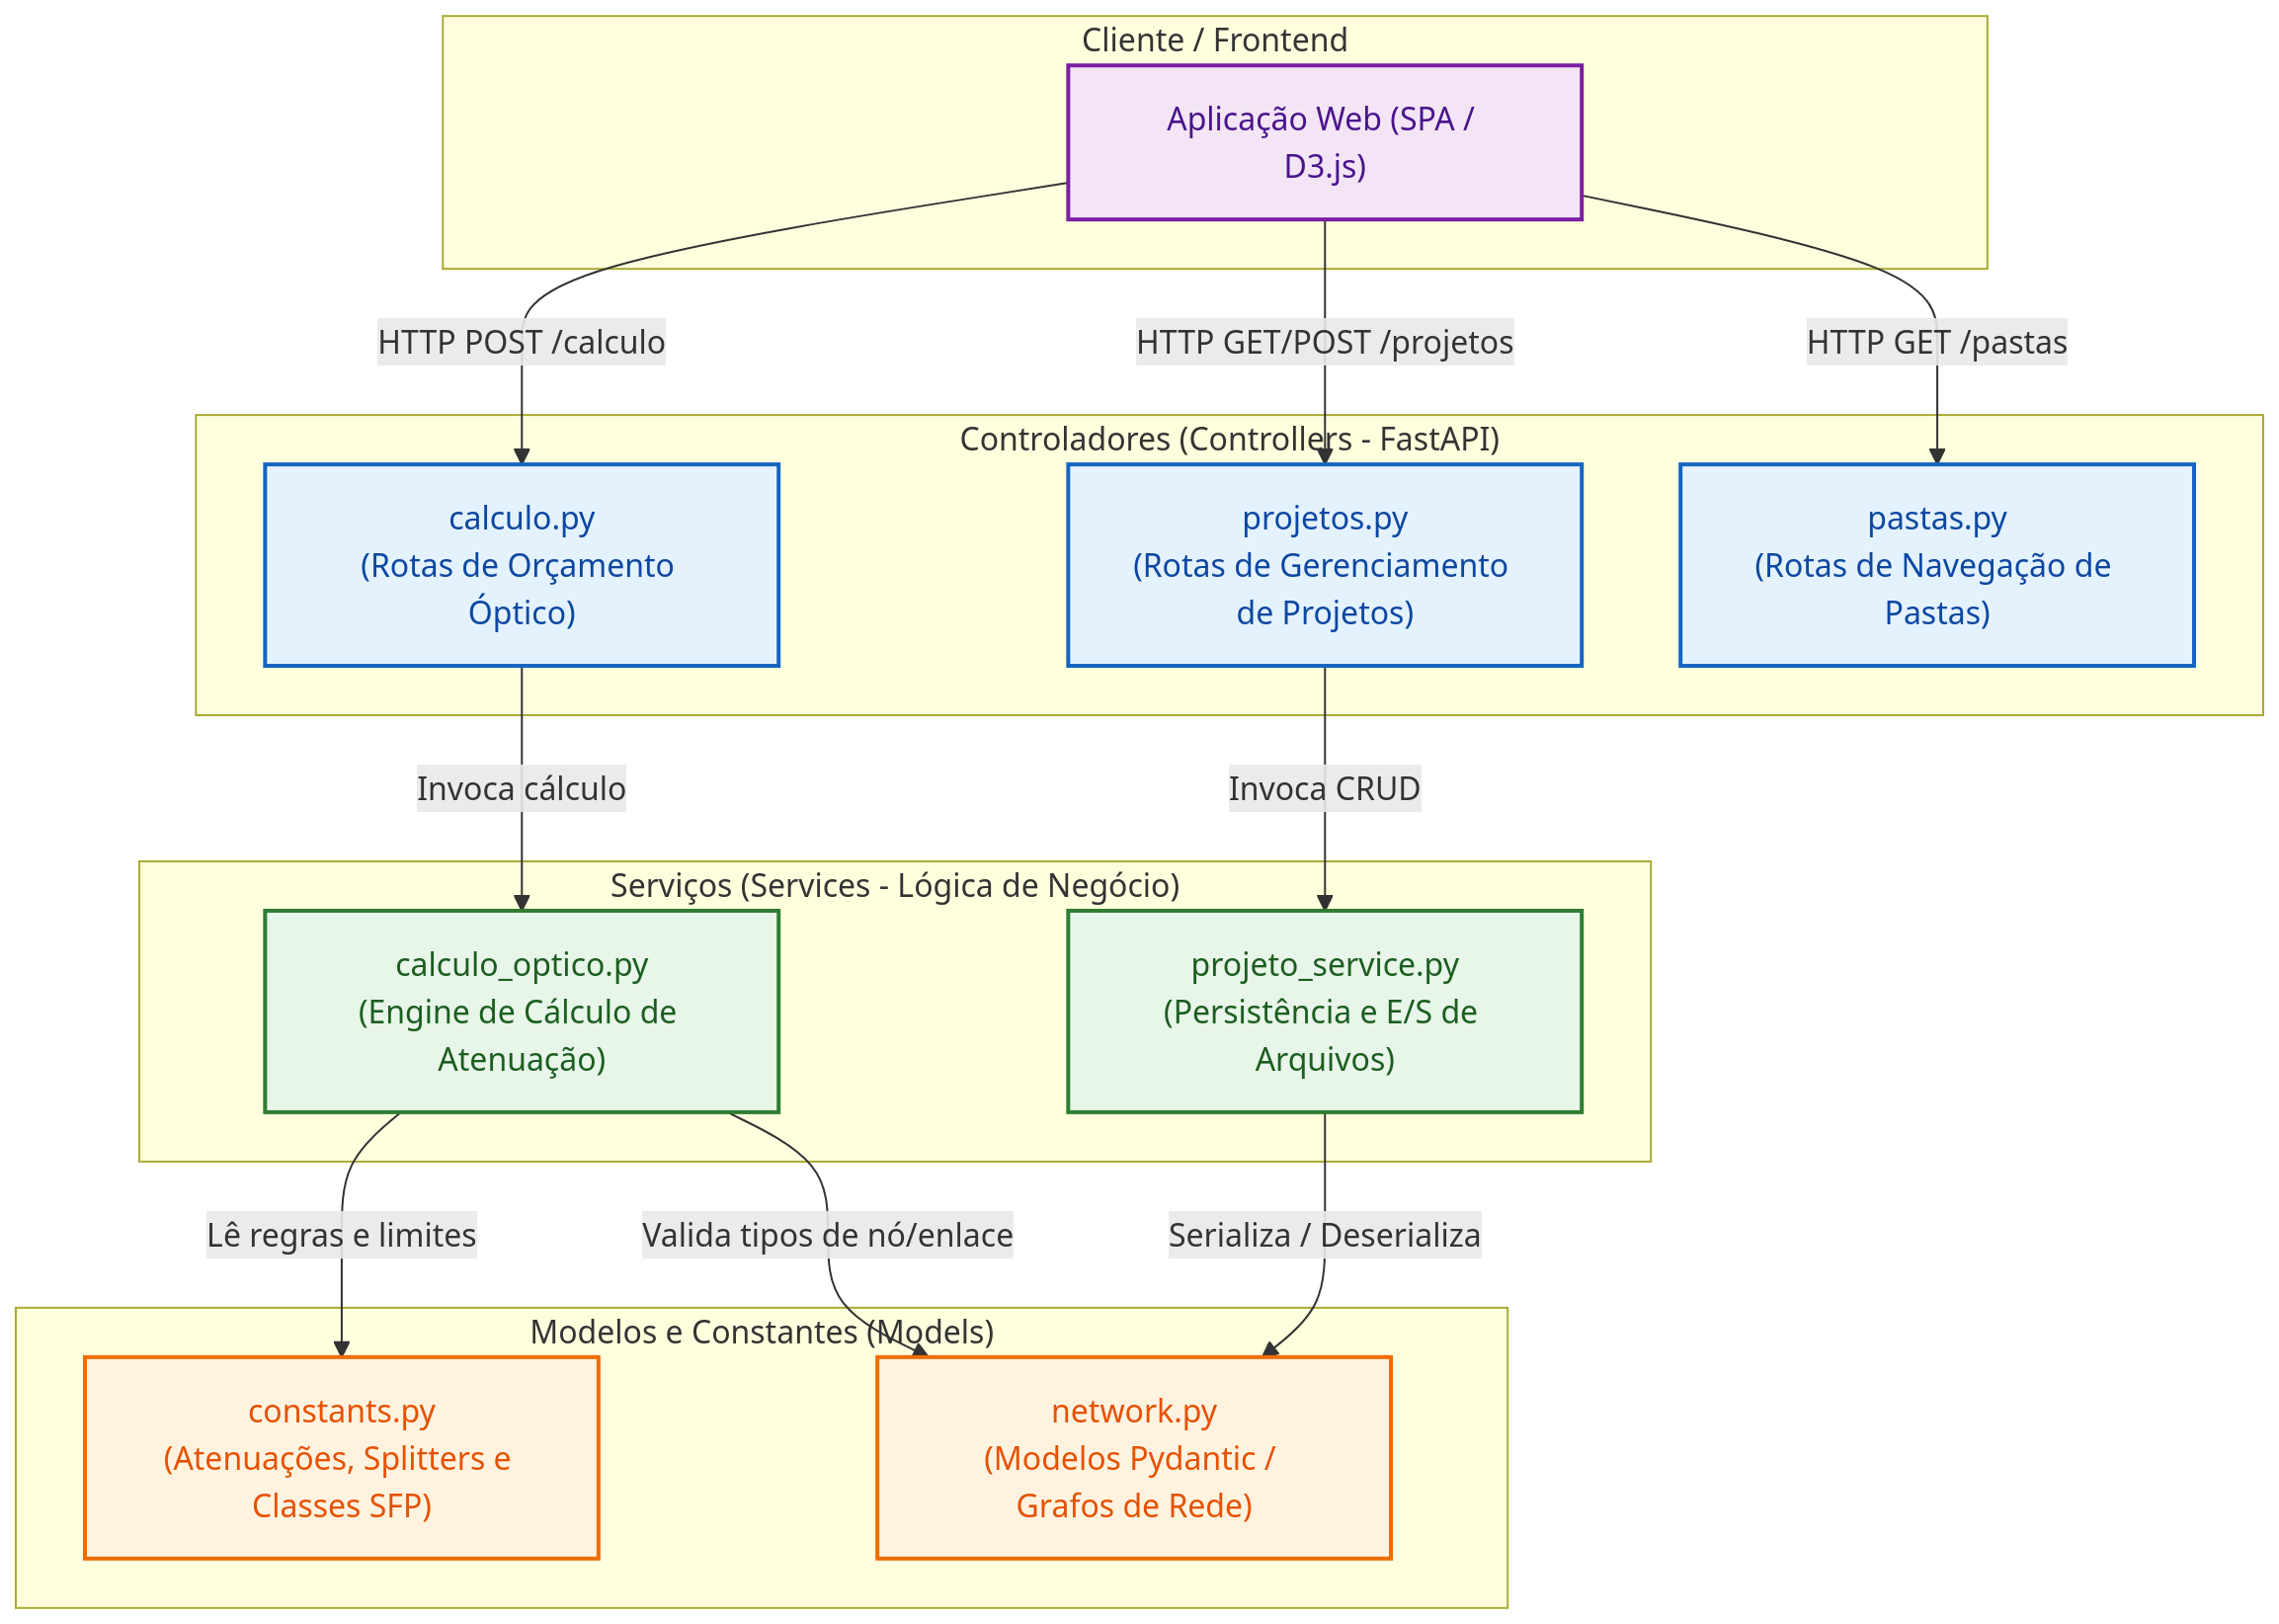
\includegraphics[width=\textwidth]{images/diagrama_componentes.png}
        \par\footnotesize Fonte: Elaboração própria com auxílio de IA.
    }
\end{figure}

\subsection{Diagrama de Implantação}

Para garantir a portabilidade e a facilidade de distribuição da plataforma, adotei a conteinerização da aplicação utilizando Docker. O ambiente é orquestrado por meio do Docker Compose, isolando a execução do servidor FastAPI e de suas dependências em um contêiner padronizado.

Na Figura~\ref{fig:diagrama_implantacao}, apresento o Diagrama de Implantação do sistema, destacando o ambiente de execução containerizado e a exposição da porta de atendimento de requisições.

\begin{figure}[htb]
    \caption{Diagrama de implantação do sistema containerizado}
    \centering
    \parbox{16cm}{
        \centering
        \label{fig:diagrama_implantacao}
        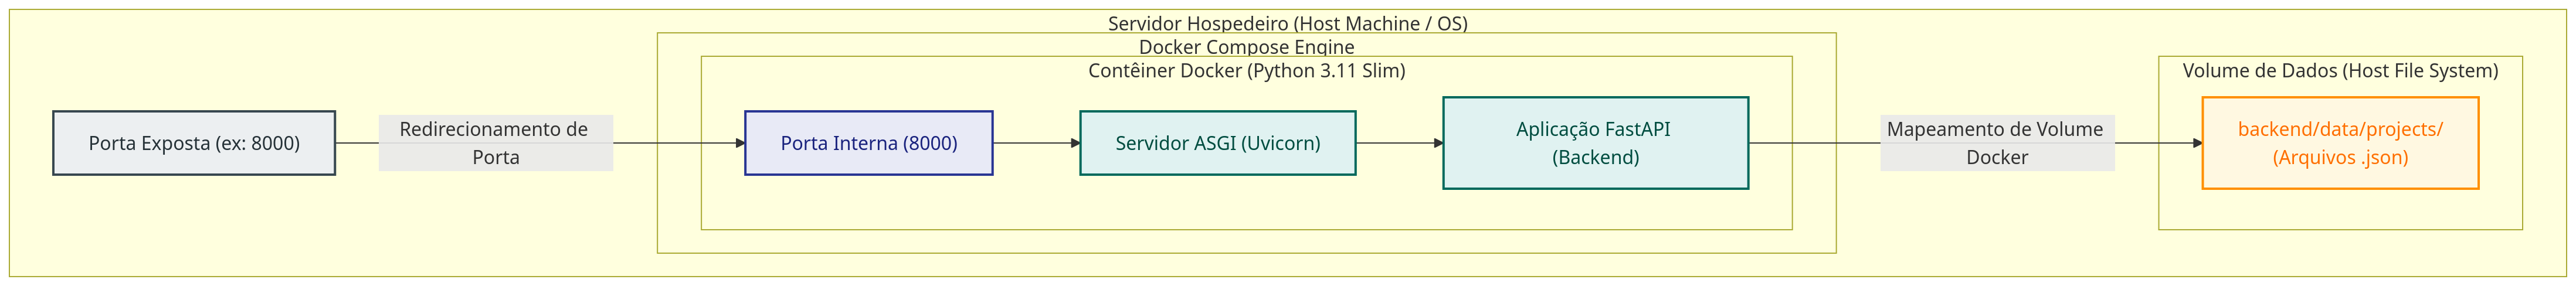
\includegraphics[width=\textwidth]{images/diagrama_implantacao.png}
        \par\footnotesize Fonte: Elaboração própria com auxílio de IA.
    }
\end{figure}

O arquivo \texttt{Dockerfile} especifica a imagem base Python, a instalação das dependências declaradas em \texttt{requirements.txt} e a inicialização do servidor de aplicação Uvicorn. O \texttt{docker-compose.yml} faz o mapeamento das portas do hospedeiro para o contêiner e configura os volumes de dados para garantir a persistência dos projetos salvos em formato \gls{json} no diretório \texttt{backend/data/projects}.

\section{Modelagem de Dados}
\label{sec:modelagem_dados}

Para a representação da topologia de rede óptica e persistência dos projetos, optei por uma estrutura de dados serializada em formato \gls{json}. Essa modelagem baseada em grafos confere leveza ao sistema e flexibilidade para a manipulação dos nós e enlaces tanto no \textit{frontend} quanto no \textit{backend}, eliminando a necessidade de um banco de dados relacional complexo. A seguir, detalho a estrutura conceitual e o esquema completo do documento de projeto.

\subsection{Modelo Conceitual e Estrutura dos Dados}

O projeto é representado por um documento \gls{json} autocontido composto por quatro blocos de dados essenciais:

\begin{itemize}
    \item \textbf{Metadados e Parâmetros Globais (\texttt{parametros}):} Define as configurações globais do projeto, incluindo atenuador padrão da fibra ($\text{dB/km}$), perda por conectorização, perda por fusão e margem de segurança do sistema em dB.
    
    \item \textbf{Nós da Rede (\texttt{nos}):} Conjunto de elementos que compõem a topologia. Cada nó possui atributos de identificação (\texttt{id}, \texttt{nome}), coordenadas de renderização espacial (\texttt{posicao}), e propriedades específicas de acordo com o seu tipo:
    \begin{itemize}
        \item \textit{\gls{olt}:} Armazena a potência de transmissão (\texttt{potencia\_tx\_dbm}), sensibilidade de recepção (\texttt{sensibilidade\_rx\_dbm}) e o padrão de rede (\texttt{padrao\_pon}).
        \item \textit{Splitter:} Suporta divisões balanceadas e desbalanceadas, registrando a razão de divisão (\texttt{razao}), a indicação do tipo (\texttt{tipo\_splitter}) e a fração desbalanceada (\texttt{razao\_desbalanceada}, ex.: 10/90, 20/80).
        \item \textit{\gls{onu}:} Ponto terminal de atendimento que especifica a sensibilidade óptica mínima exigida (\texttt{sensibilidade\_rx\_dbm}).
        \item \textit{Texto:} Elemento visual utilitário utilizado para delimitação gráfica e identificação das caixas de atendimento na interface (ex.: Caixas de Emenda, CTOs 377, 378, 379).
    \end{itemize}
    
    \item \textbf{Enlaces e Conexões (\texttt{enlaces}):} Mapeia as conexões direcionadas entre um nó de origem (\texttt{id\_origem}) e um nó de destino (\texttt{id\_destino}). Cada enlace armazena o comprimento do trecho em metros (\texttt{comprimento\_m}), a taxa de atenuação específica, o número de conexões/fusões, e a atenuação individual introduzida pelas portas dos \textit{splitters} (\texttt{perda\_splitter\_db}).
\end{itemize}

\subsection{Esquema do Arquivo JSON de Projeto}

Abaixo, apresento a estrutura de um arquivo de projeto serializado implementado no sistema, exemplificando a integração dos nós, enlaces e parâmetros globais de cálculo:

\begin{verbatim}
{
  "id": "projeto-yol156nu",
  "nome": "pon-5-1",
  "parametros": {
    "atenuacao_fibra_db_por_km": 0.35,
    "perda_conector_db": 0.5,
    "perda_fusao_db": 0.03,
    "margem_sistema_db": 3
  },
  "nos": [
    {
      "id": "olt-1",
      "tipo": "OLT",
      "nome": "pon 5/1",
      "potencia_tx_dbm": 5.0,
      "sensibilidade_rx_dbm": -28.0,
      "padrao_pon": "GPON",
      "posicao": { "x": -369.0, "y": 260.0 }
    },
    {
      "id": "splitter-2",
      "tipo": "Splitter",
      "nome": "10/90",
      "razao": 8,
      "tipo_splitter": "desbalanceado",
      "razao_desbalanceada": "10/90",
      "posicao": { "x": 230.0, "y": 256.0 }
    },
    {
      "id": "onu-3",
      "tipo": "ONU",
      "nome": "SINAL 1x8",
      "sensibilidade_rx_dbm": -27.0,
      "posicao": { "x": 262.0, "y": -43.0 }
    }
  ],
  "enlaces": [
    {
      "id": "lnk-3",
      "id_origem": "splitter-1",
      "id_destino": "splitter-2",
      "comprimento_m": 100.0,
      "atenuacao_db_por_km": 0.35,
      "tipo_conexao": "fusao",
      "num_conexoes": 2,
      "perda_por_conexao_db": 0.03,
      "perda_splitter_db": 0.36
    }
  ]
}
\end{verbatim}

Essa estrutura permite que todo o cálculo do orçamento óptico seja realizado de forma iterativa percorrendo os \textit{arrays} \texttt{nos} e \texttt{enlaces}, garantindo que atualizações de topologia sejam sincronizadas de forma ágil entre a interface visual e o motor de cálculo.

\section{Modelagem de Processos}

Nesta seção, apresento o funcionamento lógico da aplicação e o algoritmo responsável pelo processamento e cálculo do orçamento óptico ao longo da topologia de rede. A modelagem de processos descreve o fluxo de dados desde a captura das interações na interface gráfica até a execução dos cálculos matemáticos de atenuação no \textit{backend}.

\subsection{Fluxo Principal de Sinalização e Cálculo}

O fluxo de processamento é disparado de forma reativa a cada modificação realizada pelo usuário na interface gráfica. A interação segue um modelo assíncrono cliente-servidor, garantindo que o cálculo do orçamento de potência seja processado e refletido visualmente em milissegundos.

A Figura~\ref{fig:fluxo_calculo} ilustra o Diagrama de Sequência que detalha a sinalização e o fluxo de dados entre o usuário, a interface em D3.js, o controlador da \gls{api} e o motor de cálculo do \textit{backend}.

\begin{figure}[htb]
    \caption{Fluxo de sinalização e cálculo do orçamento óptico}
    \centering
    \parbox{16cm}{
        \centering
        \label{fig:fluxo_calculo}
        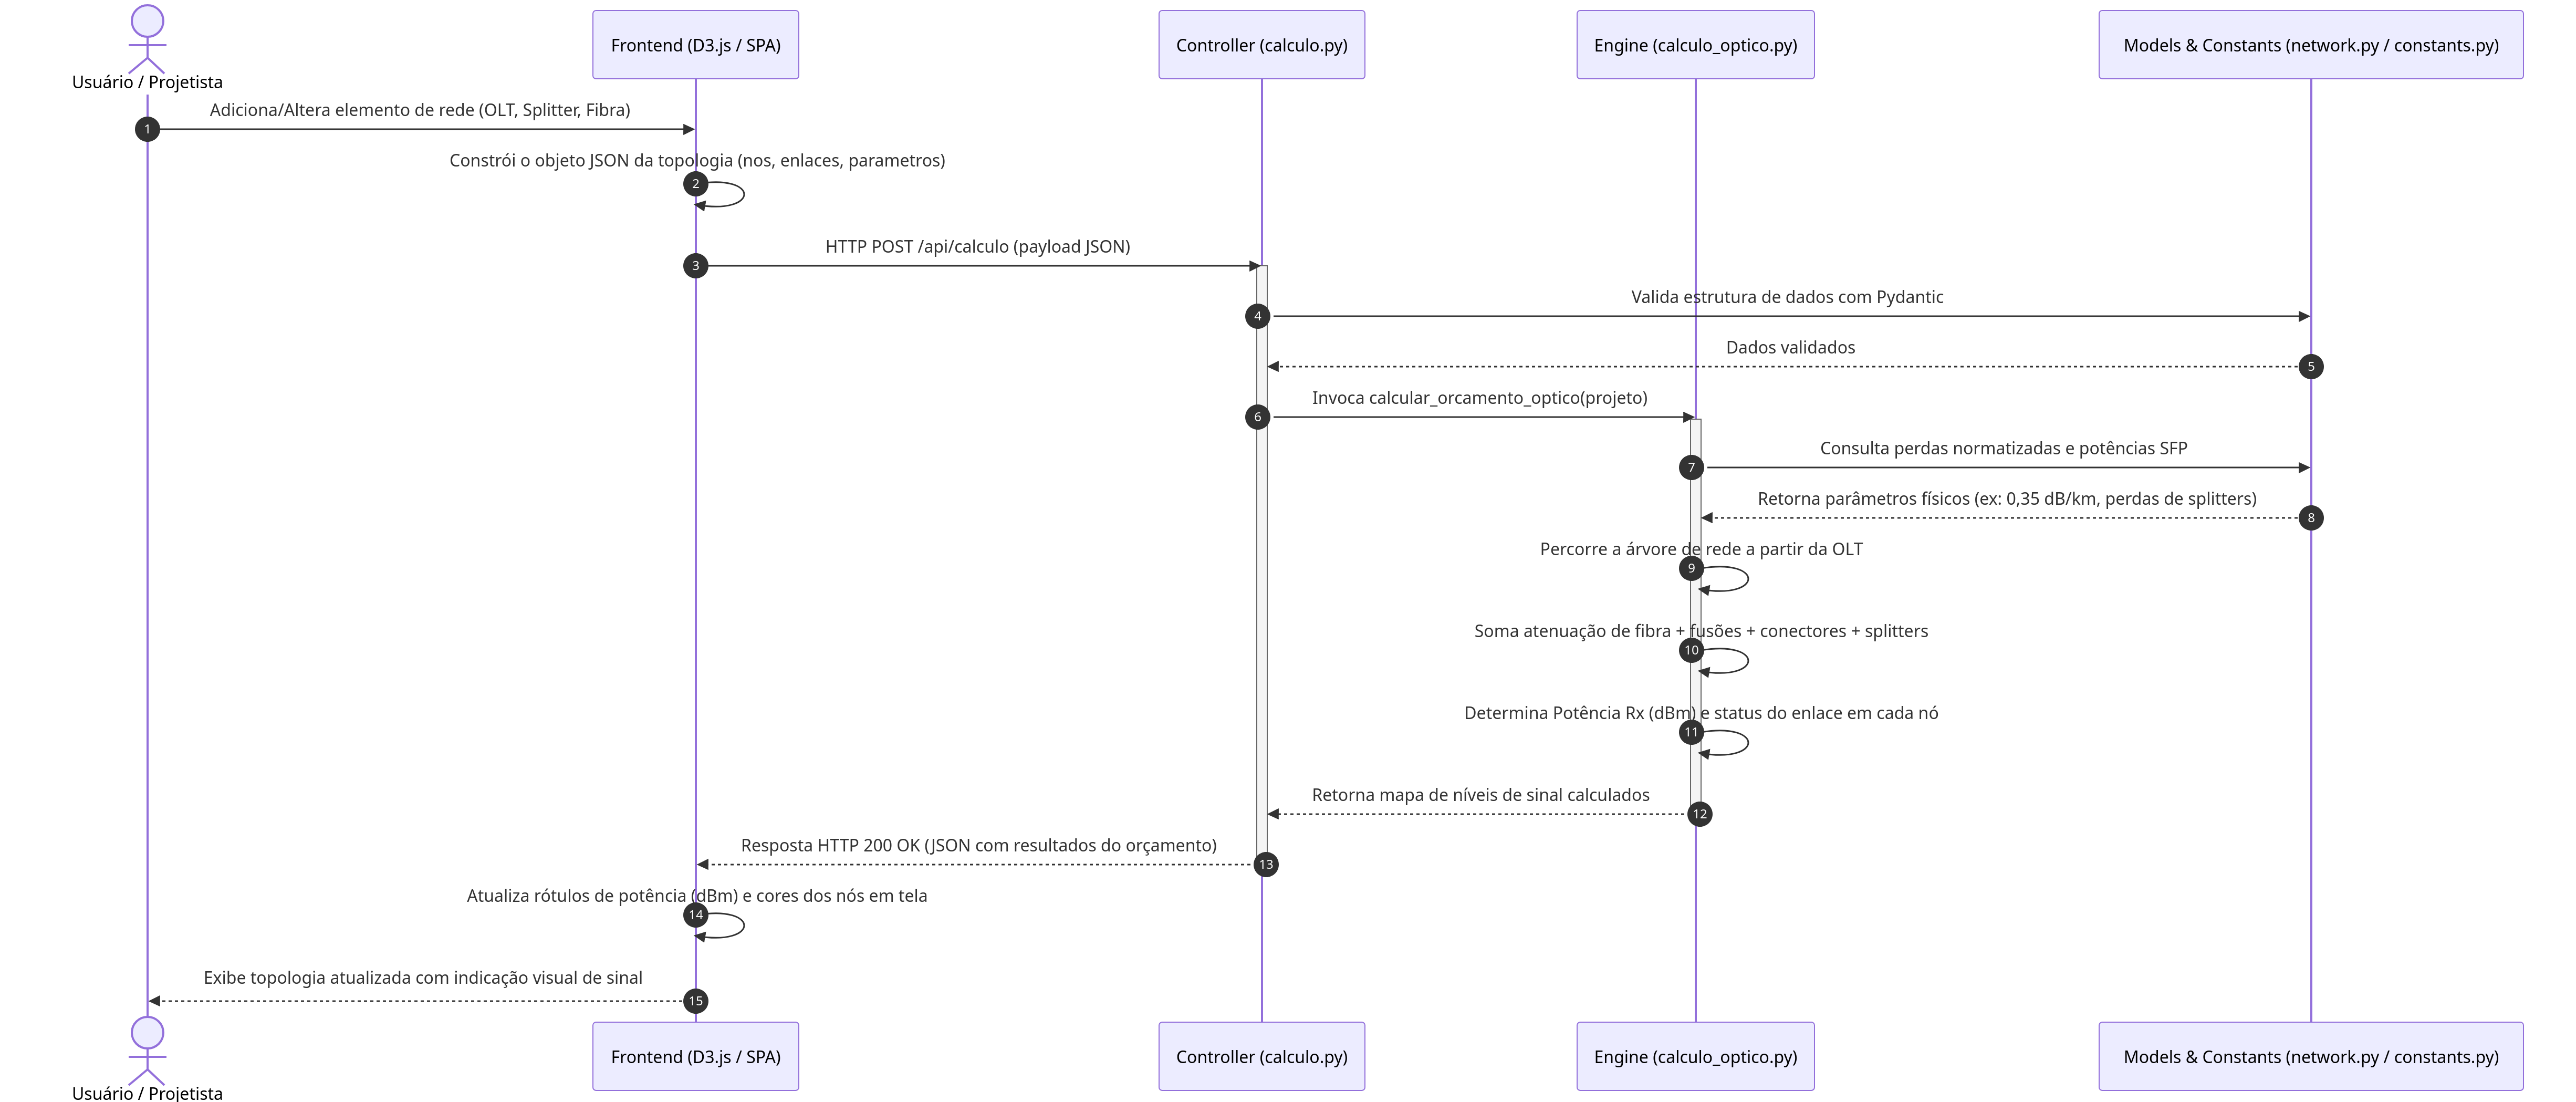
\includegraphics[width=\textwidth]{images/fluxo_calculo.png}
        \par\footnotesize Fonte: Elaboração própria com auxílio de IA.
    }
\end{figure}

O ciclo de execução ilustrado compreende as seguintes etapas encadeadas:

\begin{enumerate}
    \item \textbf{Captura da Ação:} O usuário altera a topologia (ex.: altera a distância de um cabo de fibra óptica ou altera a razão de um \textit{splitter}).
    \item \textbf{Serialização:} O \textit{frontend} lê a estrutura do grafo manipulado via D3.js e monta o documento \gls{json} padronizado com os nós, enlaces e parâmetros de rede.
    \item \textbf{Requisição HTTP:} A aplicação envia uma requisição \gls{http} \texttt{POST} assíncrona contendo o estado da rede para a rota \texttt{/api/calculo}.
    \item \textbf{Validação e Processamento:} O controlador valida os dados via Pydantic e aciona o motor de cálculo em Python (\texttt{calculo\_optico.py}), que percorre iterativamente a árvore da rede somando as perdas do trecho.
    \item \textbf{Renderização Visual:} O \textit{backend} retorna a lista de nós com seus respectivos valores de potência estimada. O \textit{frontend} atualiza imediatamente os rótulos de sinal em tela e aplica códigos de cores (verde para sinal dentro da margem, amarelo para atenção e vermelho para degradação/inoperância).
\end{enumerate}

\subsection{Algoritmo de Cálculo do Orçamento Óptico}

A lógica matemática de atenuação implementada em \texttt{calculo\_optico.py} calcula a perda acumulada ($A_{\text{total}}$) de cada caminho óptico até as terminações (\gls{onu}/\gls{cto}). A atenuação total de um enlace é dada pela soma das perdas distribuídas e concentradas, conforme a Equação:

\begin{equation}
A_{\text{total}} = (\alpha_{\text{fibra}} \cdot d) + (N_{\text{fusao}} \cdot \alpha_{\text{fusao}}) + (N_{\text{con}} \cdot \alpha_{\text{con}}) + \alpha_{\text{splitter}}
\end{equation}

Em que:
\begin{itemize}
    \item $\alpha_{\text{fibra}}$ é o coeficiente de atenuação da fibra óptica em dB/km (definido tipicamente em 0,35~dB/km);
    \item $d$ é a distância total do trecho em quilômetros;
    \item $N_{\text{fusao}}$ e $\alpha_{\text{fusao}}$ representam a quantidade de fusões/emendas e a atenuação por fusão (0,1~dB por padrão), respectivamente;
    \item $N_{\text{con}}$ e $\alpha_{\text{con}}$ representam a quantidade de conectores e a atenuação por conectorização (0,3~dB para conectores SC/APC por padrão), respectivamente;
    \item $\alpha_{\text{splitter}}$ é a perda de inserção concentrada introduzida pelos \textit{splitters} presentes no trajeto (por exemplo, $\approx 10,5$~dB para \textit{splitters} 1:8 balanceados).
\end{itemize}

Com a atenuação acumulada calculada, o nível de potência óptica incidente na \gls{onu} ($P_{\text{rx}}$) é obtido subtraindo $A_{\text{total}}$ da potência de saída do emissor da \gls{olt} ($P_{\text{tx}}$):

\begin{equation}
P_{\text{rx}} = P_{\text{tx}} - A_{\text{total}}
\end{equation}

O resultado $P_{\text{rx}}$ é comparado com os limites de sensibilidade da \gls{onu}, permitindo classificar o sinal do nó como adequado, crítico ou inoperante.

\section{Implementação dos Módulos Técnicos do Backend}
\label{sec:modulos_backend}

Nesta seção, detalho a implementação dos módulos do \textit{backend} da aplicação. O servidor foi construído em Python 3.11 utilizando o \textit{framework} FastAPI, escolhido pelo alto desempenho, suporte nativo a operações assíncronas (\textit{async/await}) e validação automática de tipos com Pydantic.

\subsection{Estrutura de Diretórios e Módulos do \textit{Backend}}

A organização física dos arquivos no repositório separa claramente as responsabilidades da aplicação entre controladores \gls{rest}, lógica de negócio e modelos de dados:

\begin{verbatim}
TCC-Redes-PON-main/
├── docker-compose.yml        # Orquestração do container (raiz do projeto)
└── backend/
    ├── Dockerfile            # Imagem de execução do backend
    ├── main.py               # Ponto de entrada do servidor FastAPI
    ├── requirements.txt      # Dependências (FastAPI, Uvicorn, Pydantic)
    ├── app/
    │   ├── controllers/      # Controladores REST (calculo.py, projetos.py)
    │   ├── services/         # Regras de negócio (calculo_optico.py, projeto_service.py)
    │   └── models/           # Esquemas Pydantic e constantes (network.py)
    ├── data/projects/        # Repositório de arquivos JSON salvos
    └── tests/                # Suíte de testes automatizados com Pytest
\end{verbatim}

\subsection{Modelagem Pydantic e Esquema de Dados (\texttt{network.py})}

A validação dos dados no servidor é feita pela biblioteca Pydantic. As estruturas foram divididas em classes específicas para garantir a tipagem correta de cada componente.

O primeiro trecho define os parâmetros globais da rede e a posição cartesiana dos nós:

\begin{verbatim}
from pydantic import BaseModel
from typing import List, Optional

class ParametrosGlobais(BaseModel):
    atenuacao_fibra_db_por_km: float = 0.35
    perda_conector_db: float = 0.5
    perda_fusao_db: float = 0.03
    margem_sistema_db: float = 3.0

class Posicao(BaseModel):
    x: float
    y: float
\end{verbatim}

A classe \texttt{ParametrosGlobais} estabelece as taxas teóricas e coeficientes de atenuação padrão utilizados na ausência de especificações nos enlaces. Já a classe \texttt{Posicao} armazena a localização espacial $(x,y)$ utilizada no \textit{canvas} gráfico.

Em seguida, o esquema detalha os atributos dos nós e conexões de fibra:

\begin{verbatim}
class NoSchema(BaseModel):
    id: str
    tipo: str  # "OLT", "Splitter", "ONU", "Texto"
    nome: str
    posicao: Posicao
    potencia_tx_dbm: Optional[float] = None
    sensibilidade_rx_dbm: Optional[float] = None
    padrao_pon: Optional[str] = None
    razao: Optional[int] = None
    tipo_splitter: Optional[str] = None  # "balanceado" ou "desbalanceado"
    razao_desbalanceada: Optional[str] = None

class EnlaceSchema(BaseModel):
    id: str
    id_origem: str
    id_destino: str
    comprimento_m: float
    atenuacao_db_por_km: float = 0.35
    tipo_conexao: str = "fusao"
    num_conexoes: int = 2
    perda_por_conexao_db: float = 0.03

class ProjetoSchema(BaseModel):
    id: str
    nome: str
    parametros: ParametrosGlobais
    nos: List[NoSchema]
    enlaces: List[EnlaceSchema]
\end{verbatim}

O \texttt{NoSchema} utiliza campos opcionais para suportar diferentes equipamentos. Por exemplo, atributos como \texttt{potencia\_tx\_dbm} são exclusivos da OLT, enquanto \texttt{razao\_desbalanceada} aplica-se apenas a \textit{splitters} ópticos. O \texttt{ProjetoSchema} consolida o documento JSON completo.

\subsection{Camada de Serviços e Algoritmo de Cálculo Óptico (\texttt{calculo\_optico.py})}

O arquivo \texttt{app/services/calculo\_optico.py} é o núcleo de cálculo do sistema. Ele interpreta a topologia como um grafo e calcula iterativamente a atenuação do sinal a partir da OLT.

A Figura~\ref{fig:fluxo_percurso_grafo} ilustra o fluxo sequencial do algoritmo de travessia do grafo e cálculo de atenuação acumulada.

\begin{figure}[htb]
    \caption{Fluxograma do algoritmo de travessia do grafo e cálculo óptico}
    \centering
    \parbox{16cm}{
        \centering
        \label{fig:fluxo_percurso_grafo}
        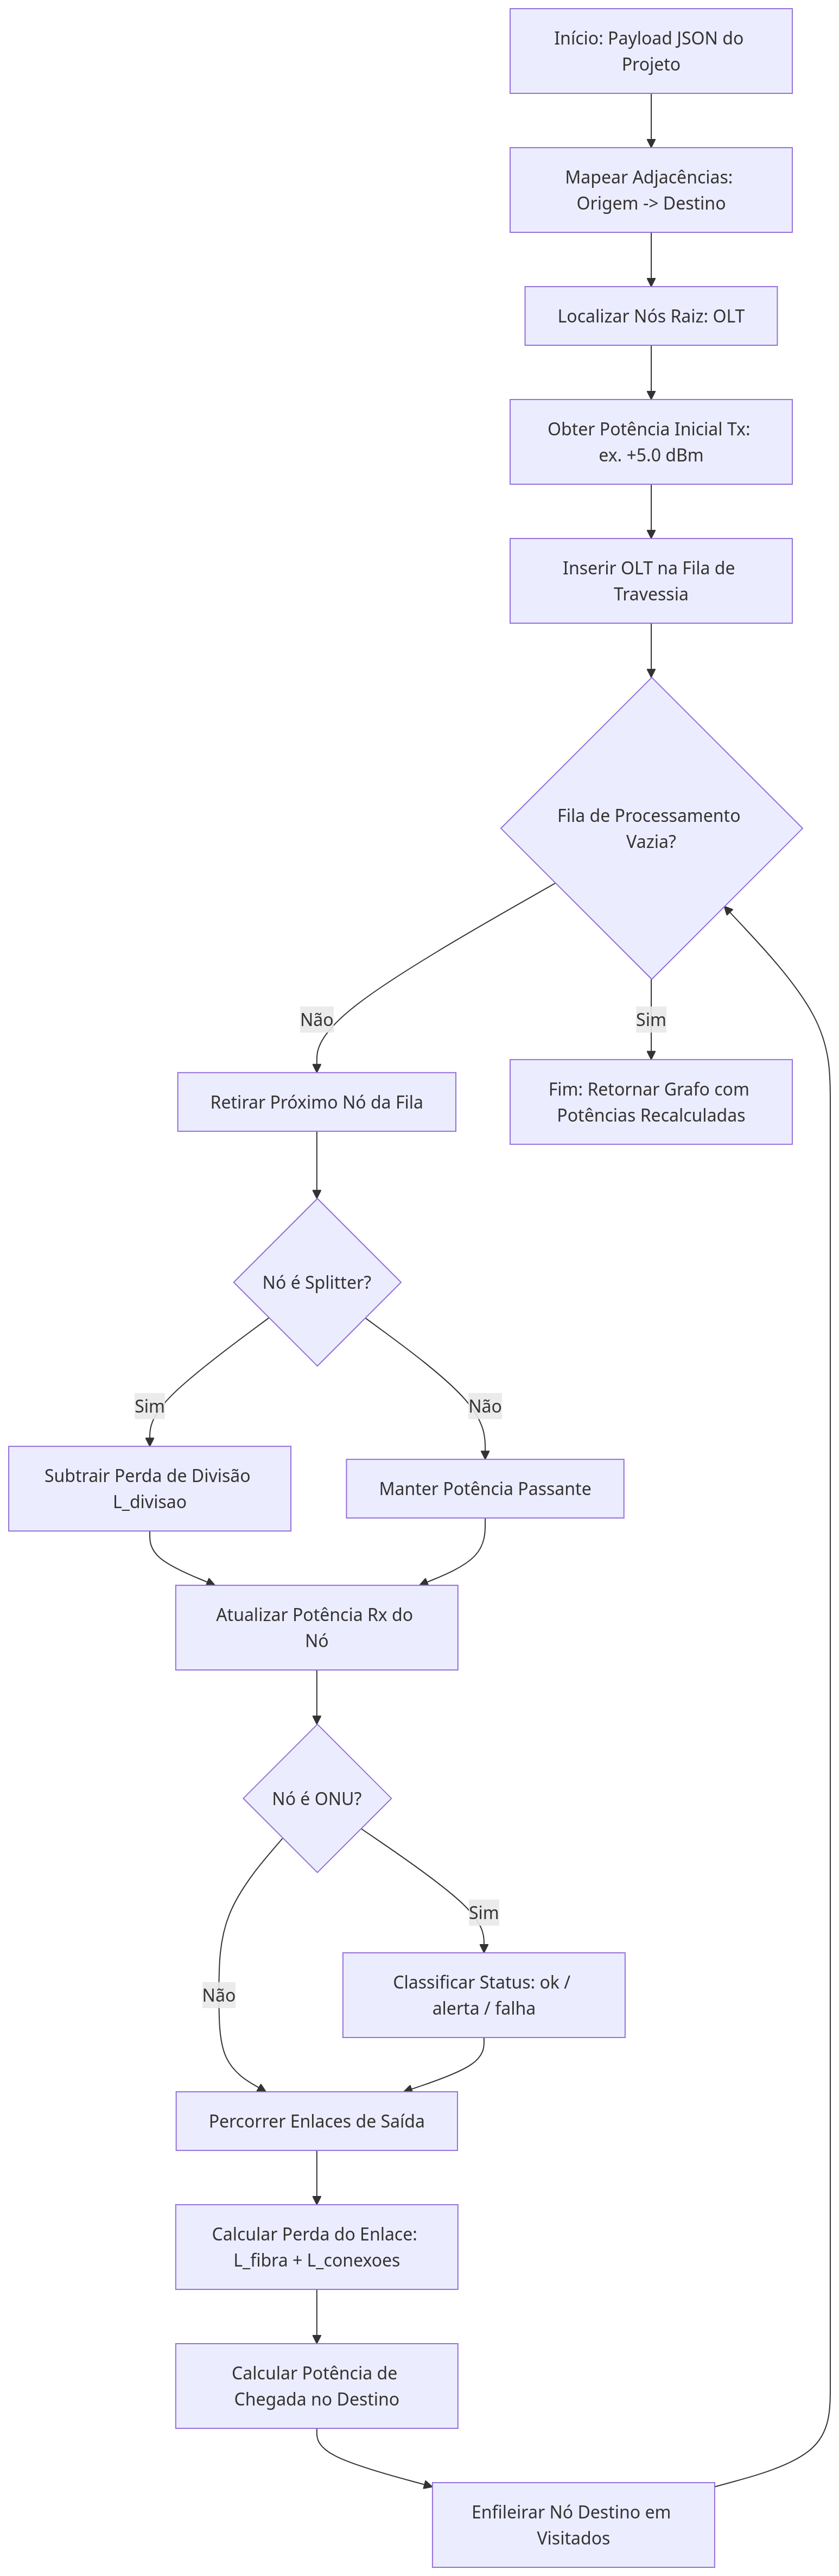
\includegraphics[width=0.35\textwidth]{images/fluxo_percurso_grafo.png}
        \par\footnotesize Fonte: Elaboração própria com auxílio de IA.
    }
\end{figure}

A implementação do motor de cálculo é dividida em três fases principais. A primeira fase realiza a montagem do mapa de adjacências e localiza o nó raiz:

\begin{verbatim}
import math
from typing import Dict, Any, List
from app.models.network import ProjetoSchema
from app.models.constants import PERDAS_SPLITTER_BALANCEADO, PERDAS_SPLITTER_DESBALANCEADO

def calcular_orcamento_optico(projeto: ProjetoSchema) -> Dict[str, Any]:
    nos_dict = {no.id: no.dict() for no in projeto.nos}
    
    # Mapeia as conexões de saída: id_origem -> lista de (enlace, id_destino)
    adjacencias: Dict[str, List[tuple]] = {no.id: [] for no in projeto.nos}
    for enlace in projeto.enlaces:
        if enlace.id_origem in adjacencias:
            adjacencias[enlace.id_origem].append((enlace, enlace.id_destino))

    # Identifica o nó emissor (OLT)
    olt = next((no for no in projeto.nos if no.tipo == "OLT"), None)
    if not olt:
        raise ValueError("A topologia não possui uma OLT cadastrada como raiz.")

    potencia_inicial = olt.potencia_tx_dbm if olt.potencia_tx_dbm is not None else 5.0
    nos_dict[olt.id]["potencia_rx"] = potencia_inicial
    nos_dict[olt.id]["status_sinal"] = "ok"
\end{verbatim}

Esta etapa converte a lista de enlaces em um dicionário de adjacências otimizado, permitindo que o algoritmo consulte as ramificações de saída de qualquer nó.

A segunda fase executa a travessia da rede utilizando uma fila de processamento:

\begin{verbatim}
    fila = [(olt.id, potencia_inicial)]
    visitados = set()

    while fila:
        no_atual_id, potencia_atual = fila.pop(0)
        visitados.add(no_atual_id)
        no_atual = nos_dict[no_atual_id]

        # Desconta a perda interna caso o nó seja um Splitter
        perda_interna_no = 0.0
        if no_atual["tipo"] == "Splitter":
            perda_interna_no = obter_perda_splitter(no_atual)

        potencia_apos_no = potencia_atual - perda_interna_no
        no_atual["potencia_rx"] = round(potencia_apos_no, 2)

        # Classifica o estado do sinal se o nó for uma ONU
        if no_atual["tipo"] == "ONU":
            sensibilidade = no_atual.get("sensibilidade_rx_dbm") or -27.0
            if potencia_apos_no >= sensibilidade:
                no_atual["status_sinal"] = "ok"
            elif potencia_apos_no >= (sensibilidade + projeto.parametros.margem_sistema_db):
                no_atual["status_sinal"] = "alerta"
            else:
                no_atual["status_sinal"] = "falha"
\end{verbatim}

Durante o laço, a atenuação do nó é subtraída do sinal incidente. Caso o nó seja uma ONU, o valor final $P_{\text{rx}}$ é comparado com o limiar de sensibilidade, atribuindo o estado funcional (\texttt{ok}, \texttt{alerta} ou \texttt{falha}).

A terceira fase estende a propagação do sinal ao longo dos enlaces conectados:

\begin{verbatim}
        # Propaga o sinal para os nós sucessores através dos enlaces de fibra
        for enlace, id_destino in adjacencias.get(no_atual_id, []):
            distancia_km = enlace.comprimento_m / 1000.0
            perda_fibra = distancia_km * enlace.atenuacao_db_por_km
            perda_conexoes = enlace.num_conexoes * enlace.perda_por_conexao_db
            
            perda_total_enlace = perda_fibra + perda_conexoes
            potencia_destino = potencia_apos_no - perda_total_enlace

            if id_destino not in visitados:
                fila.append((id_destino, potencia_destino))

    return {
        "nos": list(nos_dict.values()),
        "enlaces": [e.dict() for e in projeto.enlaces]
    }
\end{verbatim}

Para cada enlace, o código calcula a atenuação por quilometragem somada às perdas de acoplamentos mecânicos ou fusões. O resultado atualizado da potência é enfileirado para o próximo nó destino.

A função auxiliar para o cálculo de perda em \textit{splitters} é detalhada a seguir:

\begin{verbatim}
def obter_perda_splitter(no: dict) -> float:
    tipo = no.get("tipo_splitter", "balanceado")
    if tipo == "balanceado":
        razao = no.get("razao", 8)
        return PERDAS_SPLITTER_BALANCEADO.get(razao, 10.0 * math.log10(razao) + 0.5)
    elif tipo == "desbalanceado":
        razao_str = no.get("razao_desbalanceada", "10/90")
        return PERDAS_SPLITTER_DESBALANCEADO.get(razao_str, {}).get("passagem", 1.5)
    return 0.0
\end{verbatim}

\subsection{Serviços de Controladores e Persistência de Dados}

O controlador \gls{rest} \texttt{app/controllers/calculo.py} atua como intermediário entre a Web e a camada de serviço:

\begin{verbatim}
from fastapi import APIRouter, HTTPException, status
from app.models.network import ProjetoSchema
from app.services.calculo_optico import calcular_orcamento_optico

router = APIRouter(prefix="/api/calculo", tags=["Cálculo Óptico"])

@router.post("", status_code=status.HTTP_200_OK)
async def processar_calculo(projeto: ProjetoSchema):
    try:
        resultado = calcular_orcamento_optico(projeto)
        return {"status": "sucesso", "dados": resultado}
    except Exception as exc:
        raise HTTPException(
            status_code=status.HTTP_400_BAD_REQUEST,
            detail=f"Erro ao processar cálculo óptico: {str(exc)}"
        )
\end{verbatim}

Já a persistência dos arquivos \gls{json} no disco é realizada pelo serviço \texttt{ProjetoService} (\texttt{app/services/projeto\_service.py}):

\begin{verbatim}
import os
import json
from typing import List, Optional
from app.models.network import ProjetoSchema

CAMINHO_PROJETOS = os.path.join(os.path.dirname(__file__), "../../data/projects")

class ProjetoService:
    def __init__(self):
        os.makedirs(CAMINHO_PROJETOS, exist_ok=True)

    def obter_por_id(self, projeto_id: str) -> Optional[dict]:
        caminho = os.path.join(CAMINHO_PROJETOS, f"{projeto_id}.json")
        if not os.path.exists(caminho):
            return None
        with open(caminho, "r", encoding="utf-8") as f:
            return json.load(f)

    def salvar(self, projeto: ProjetoSchema) -> dict:
        caminho = os.path.join(CAMINHO_PROJETOS, f"{projeto.id}.json")
        with open(caminho, "w", encoding="utf-8") as f:
            json.dump(projeto.dict(), f, indent=4, ensure_ascii=False)
        return {"status": "sucesso", "id": projeto.id}
\end{verbatim}


\section{Implementação da Interface do Usuário (\textit{frontend})}

Nesta seção, apresento a implementação da interface gráfica do usuário. O \textit{frontend} foi construído sob o conceito de \gls{spa} centralizado no diretório \texttt{frontend/public/index.html}, utilizando a biblioteca D3.js (v7) para renderizaçao vetorial \gls{svg}.

\subsection{Mapeamento DOM e Estrutura de Elementos D3.js}

A renderização gráfica conecta os dados do estado JavaScript diretamente aos elementos visuais \gls{svg}. 

A Figura~\ref{fig:estrutura_d3_canvas} ilustra o mapeamento dos dados da topologia em elementos do DOM \gls{svg}.

\begin{figure}[htb]
    \caption{Mapeamento dos objetos de rede para elementos vetoriais \gls{svg} com D3.js}
    \centering
    \parbox{16cm}{
        \centering
        \label{fig:estrutura_d3_canvas}
        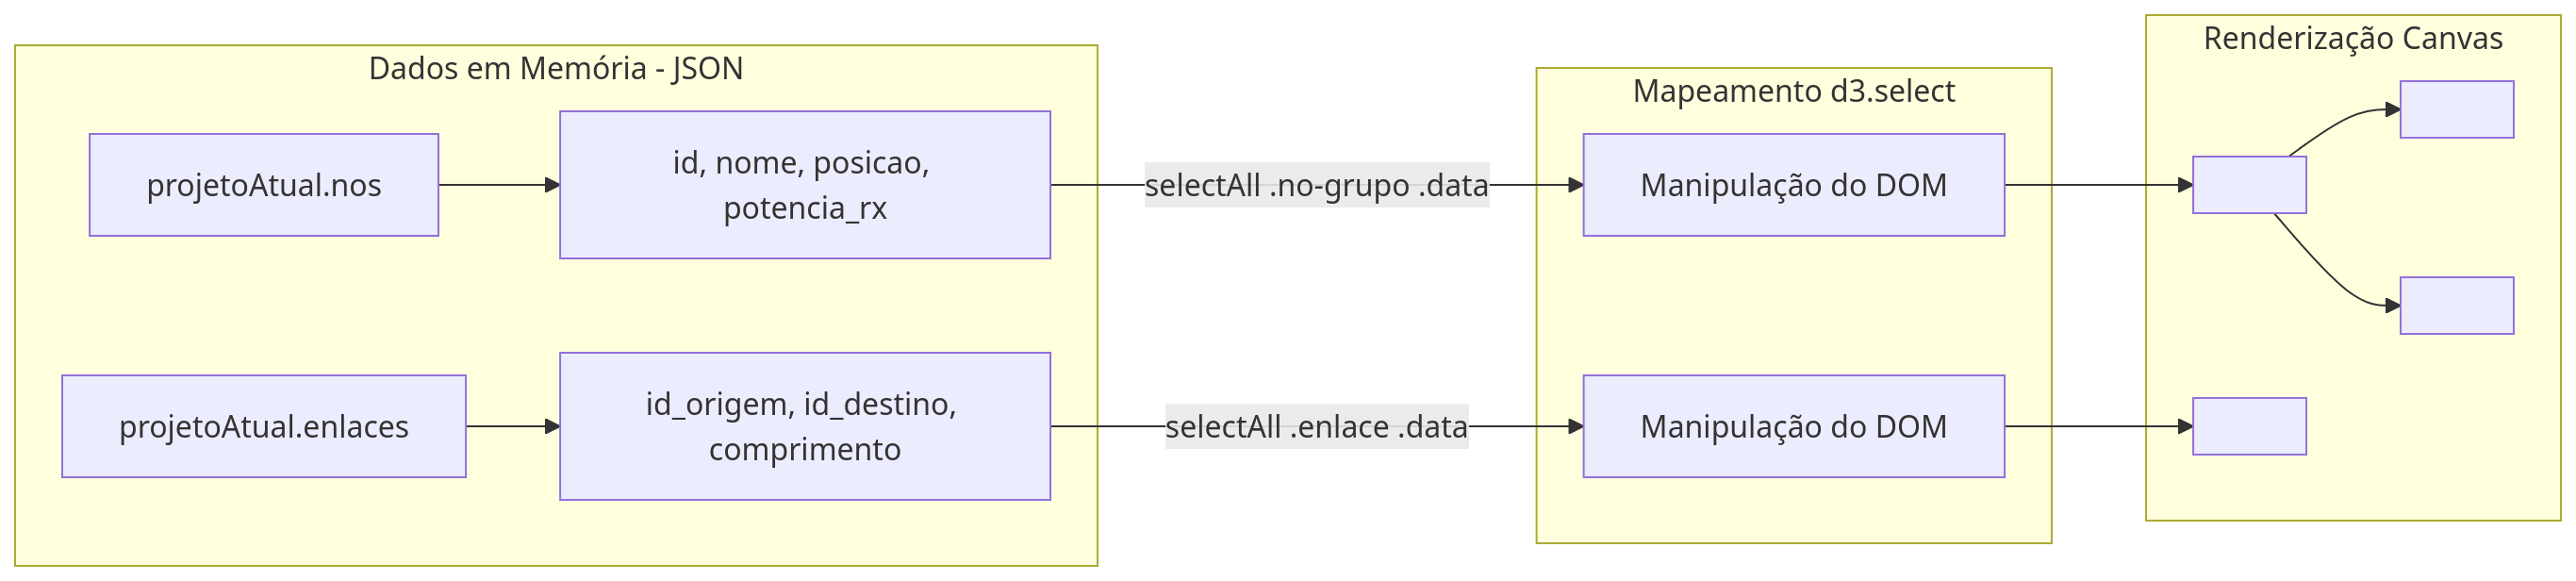
\includegraphics[width=0.85\textwidth]{images/estrutura_d3_canvas.png}
        \par\footnotesize Fonte: Elaboração própria com auxílio de IA.
    }
\end{figure}

O trecho de código a seguir demonstra o processo de renderização dos enlaces de fibra óptica:

\begin{verbatim}
// Desenho e atualização dos enlaces no contêiner SVG (<line>)
const enlaces = svg.selectAll(".enlace")
    .data(dadosProjeto.enlaces, d => d.id);

enlaces.enter()
    .append("line")
    .attr("class", "enlace")
    .merge(enlaces)
    .attr("x1", d => obterNoPorId(d.id_origem).posicao.x)
    .attr("y1", d => obterNoPorId(d.id_origem).posicao.y)
    .attr("x2", d => obterNoPorId(d.id_destino).posicao.x)
    .attr("y2", d => obterNoPorId(d.id_destino).posicao.y)
    .attr("stroke", "#0288d1")
    .attr("stroke-width", 2);

enlaces.exit().remove();
\end{verbatim}

O método \texttt{selectAll().data()} associa cada registro do \textit{array} de enlaces a uma tag \texttt{<line>} \gls{svg}. Durante a atualização, as coordenadas $(x_1, y_1)$ e $(x_2, y_2)$ são recalculadas com base nos nós de origem e destino.

Em seguida, o código cria os grupos de nós e adiciona o suporte ao arrasto (\textit{drag-and-drop}):

\begin{verbatim}
// Criação dos grupos de nós (<g>) com interatividade
const nos = svg.selectAll(".no-grupo")
    .data(dadosProjeto.nos, d => d.id);

const nosEnter = nos.enter()
    .append("g")
    .attr("class", "no-grupo")
    .call(d3.drag().on("drag", noArrastado));

nosEnter.append("circle")
    .attr("r", 18)
    .attr("fill", d => obterCorStatusSinal(d));

nosEnter.append("text")
    .attr("dy", 30)
    .attr("text-anchor", "middle")
    .text(d => `${d.nome} ${d.potencia_rx ? '(' + d.potencia_rx.toFixed(2) + ' dBm)' : ''}`);

nos.merge(nosEnter)
    .attr("transform", d => `translate(${d.posicao.x}, ${d.posicao.y})`);

nos.exit().remove();
\end{verbatim}

Cada nó é encapsulado em uma tag de grupo \texttt{<g>}, contendo um elemento \texttt{<circle>} (cuja cor reflete o status de sinal) e um elemento \texttt{<text>} (que exibe a potência calculada em dBm).

A movimentação dos nós na tela é tratada pela função \texttt{noArrastado}:

\begin{verbatim}
function noArrastado(event, d) {
    d.posicao.x = event.x;
    d.posicao.y = event.y;
    d3.select(this).attr("transform", `translate(${d.posicao.x}, ${d.posicao.y})`);
    atualizarLinhasEnlaces();
}
\end{verbatim}

\subsection{Comunicação Assíncrona e Reatividade}

A reatividade do sistema ocorre pelo envio assíncrono do estado do grafo para a \gls{api} FastAPI através do método \texttt{fetch}:

\begin{verbatim}
async function calcularOrcamentoOptico() {
    try {
        const response = await fetch('/api/calculo', {
            method: 'POST',
            headers: { 'Content-Type': 'application/json' },
            body: JSON.stringify(projetoAtual)
        });

        if (!response.ok) {
            throw new Error(`Erro na requisição: ${response.statusText}`);
        }

        const resposta = await response.json();

        if (resposta.status === 'sucesso') {
            atualizarValoresPotencia(resposta.dados.nos);
            atualizarGrafo(projetoAtual);
        }
    } catch (erro) {
        console.error("Erro ao sincronizar orçamento óptico:", erro);
    }
}
\end{verbatim}

Sempre que o usuário move um nó ou altera uma propriedade no painel lateral, esta função transmite o \gls{json} do projeto e aplica o resultado retornado sem a necessidade de recarregar a página web.
\include{conteudo/conclusao}

% ----------------------------------------------------------
% ELEMENTOS PÓS-TEXTUAIS
% ----------------------------------------------------------
\postextual

% REFERÊNCIAS BIBLIOGRÁFICAS
\bibliography{referencias}

% APÊNDICES E ANEXOS (Descomentar se for usar)
% \include{postextuais/apendice}
% \include{postextuais/anexo}

\end{document}